\documentclass{mimosis}

\usepackage{metalogo}

%%%%%%%%%%%%%%%%%%%%%%%%%%%%%%%%%%%%%%%%%%%%%%%%%%%%%%%%%%%%%%%%%%%%%%%%
% Some of my favourite personal adjustments
%%%%%%%%%%%%%%%%%%%%%%%%%%%%%%%%%%%%%%%%%%%%%%%%%%%%%%%%%%%%%%%%%%%%%%%%
%
% These are the adjustments that I consider necessary for typesetting
% a nice thesis. However, they are *not* included in the template, as
% I do not want to force you to use them.

% This ensures that I am able to typeset bold font in table while still aligning the numbers
% correctly.
\usepackage{etoolbox}

%%%%%%%%%%%%%%%%%%%%%%%%%%%%%%%%%%%%%%%%%%%%%%%%%%%%%%%%%%%%%%%%%%%%%%%%
% Hyperlinks & bookmarks
%%%%%%%%%%%%%%%%%%%%%%%%%%%%%%%%%%%%%%%%%%%%%%%%%%%%%%%%%%%%%%%%%%%%%%%%

\usepackage[%
  colorlinks = true,
  citecolor  = RoyalBlue,
  linkcolor  = RoyalBlue,
  urlcolor   = RoyalBlue,
  unicode,
  ]{hyperref}

\usepackage{bookmark}

%%%%%%%%%%%%%%%%%%%%%%%%%%%%%%%%%%%%%%%%%%%%%%%%%%%%%%%%%%%%%%%%%%%%%%%%
% Bibliography
%%%%%%%%%%%%%%%%%%%%%%%%%%%%%%%%%%%%%%%%%%%%%%%%%%%%%%%%%%%%%%%%%%%%%%%%
%
% I like the bibliography to be extremely plain, showing only a numeric
% identifier and citing everything in simple brackets. The first names,
% if present, will be initialized. DOIs and URLs will be preserved.

\usepackage[%
  autocite     = plain,
  backend      = bibtex,
  doi          = true,
  url          = true,
  giveninits   = true,
  hyperref     = true,
  maxbibnames  = 99,
  maxcitenames = 99,
  sortcites    = true,
  style        = numeric,
  ]{biblatex}

\input{bibliography-mimosis}
\addbibresource{Thesis.bib}

%%%%%%%%%%%%%%%%%%%%%%%%%%%%%%%%%%%%%%%%%%%%%%%%%%%%%%%%%%%%%%%%%%%%%%%%
% Fonts
%%%%%%%%%%%%%%%%%%%%%%%%%%%%%%%%%%%%%%%%%%%%%%%%%%%%%%%%%%%%%%%%%%%%%%%%


\usepackage{todonotes}

\setsansfont{IBM Plex Sans}
\setmonofont{IBM Plex Mono}

%%%%%%%%%%%%%%%%%%%%%%%%%%%%%%%%%%%%%%%%%%%%%%%%%%%%%%%%%%%%%%%%%%%%%%%%
% Figures
%%%%%%%%%%%%%%%%%%%%%%%%%%%%%%%%%%%%%%%%%%%%%%%%%%%%%%%%%%%%%%%%%%%%%%%%
\usepackage{import}
\usepackage{xifthen}
\usepackage{pdfpages}
\usepackage{transparent}

%%%%%%%%%%%%%%%%%%%%%%%%%%%%%%%%%%%%%%%%%%%%%%%%%%%%%%%%%%%%%%%%%%%%%%%%
% Ordinals
%%%%%%%%%%%%%%%%%%%%%%%%%%%%%%%%%%%%%%%%%%%%%%%%%%%%%%%%%%%%%%%%%%%%%%%%

\makeatletter
\@ifundefined{st}{%
  \newcommand{\st}{\textsuperscript{\textup{st}}\xspace}
}{}
\@ifundefined{rd}{%
  \newcommand{\rd}{\textsuperscript{\textup{rd}}\xspace}
}{}
\@ifundefined{nd}{%
  \newcommand{\nd}{\textsuperscript{\textup{nd}}\xspace}
}{}
\makeatother

\renewcommand{\th}{\textsuperscript{\textup{th}}\xspace}

%%%%%%%%%%%%%%%%%%%%%%%%%%%%%%%%%%%%%%%%%%%%%%%%%%%%%%%%%%%%%%%%%%%%%%%%
% Colors
%%%%%%%%%%%%%%%%%%%%%%%%%%%%%%%%%%%%%%%%%%%%%%%%%%%%%%%%%%%%%%%%%%%%%%%%
\definecolor{cRed}{HTML}{E75151}
\definecolor{cBlue}{HTML}{4F8FE0}
\definecolor{cGreen}{HTML}{65AC59}
\definecolor{cPurple}{HTML}{8863A8}
\definecolor{cOrange}{HTML}{F28D34}
\definecolor{cGrey}{HTML}{A0A0A0}
\definecolor{cBrown}{HTML}{A9795C}
\definecolor{cPink}{HTML}{F084B6}

%%%%%%%%%%%%%%%%%%%%%%%%%%%%%%%%%%%%%%%%%%%%%%%%%%%%%%%%%%%%%%%%%%%%%%%%
% Math
%%%%%%%%%%%%%%%%%%%%%%%%%%%%%%%%%%%%%%%%%%%%%%%%%%%%%%%%%%%%%%%%%%%%%%%%
\usepackage{tensors}
\usepackage{algorithm}
\usepackage{algpseudocode}

\renewcommand{\algorithmicrequire}{\textbf{Input:}}
\renewcommand{\algorithmicensure}{\textbf{Output:}}

\newcommand{\K}{\mathbb{K}}
\newcommand{\R}{\mathbb{R}}
\newcommand{\N}{\mathbb{N}}
\newcommand{\Z}{\mathbb{Z}}
\newcommand{\Q}{\mathbb{Q}}
\newcommand{\C}{\mathbb{C}}
\newcommand{\PP}{\mathbb{P}}
\newcommand{\V}{\mathcal{V}}
\newcommand{\E}{\mathcal{E}}
\newcommand{\G}{\mathcal{G}}
\newcommand{\s}{\mathcal{S}}
\renewcommand{\L}{\mathbb{L}}

\newcommand{\defeq}{\vcentcolon=}
\newcommand{\eqdef}{=\vcentcolon}
\newcommand{\norm}[1]{\left\lVert#1\right\rVert}
\newcommand{\intR}[2][\bm{v}]{\int_{\R^{#1}} #2 \, dP}
% Operators are declared in the class file (mimosis.cls)

\newtheorem{theorem}{Teorema}[section]
\newtheorem{lemma}[theorem]{Lemma}
\newtheorem{proposition}[theorem]{Proposizione}
\newtheorem{corollary}[theorem]{Corollario}
\theoremstyle{definition}
\newtheorem{definition}[theorem]{Definizione}
\newtheorem{example}[theorem]{Esempio}
\theoremstyle{remark}
\newtheorem{remark}[theorem]{Osservazione}
\NewEnviron{notation}{%
  \par\vspace{1ex}       % Small space before the environment
  \noindent\uline{\textit{Notazione:}} \BODY
  \par\vspace{1ex}       % Small space after the environment
}

%%%%%%%%%%%%%%%%%%%%%%%%%%%%%%%%%%%%%%%%%%%%%%%%%%%%%%%%%%%%%%%%%%%%%%%%
% Acronyms & Glossaries
%%%%%%%%%%%%%%%%%%%%%%%%%%%%%%%%%%%%%%%%%%%%%%%%%%%%%%%%%%%%%%%%%%%%%%%%

% --- ACRONIMI ---
\newacronym[description={Canonical Polyadic Decomposition}]{CP}{CP}{canonical polyadic decomposition}
\newacronym[description={Alternating Least Squares}]{ALS}{ALS}{alternating least squares}
\newacronym[description={Singular Value Decomposition}]{SVD}{SVD}{singular value decomposition}
\newacronym[description={Arbitrary Precision Approximating}]{APA}{APA}{arbitrary precision approximating}
\newacronym[description={Excitation-Emission Matrix}]{EEM}{EEM}{excitation-emission matrix}
\newacronym[description={Direct-Sequence Code-Division Multiple Access}]{DS-CDMA}{DS-CDMA}{direct-sequence code-division multiple access}
\newacronym[description={Blind Source Separation}]{BSS}{BSS}{blind source separation}
\newacronym[description={Signal-to-Noise Ratio}]{SNR}{SNR}{signal-to-noise ratio}
\newacronym[description={Interchip Interference}]{ICI}{ICI}{interchip interference}
\newacronym[description={Intersignal Interference}]{ISI}{ISI}{intersignal interference}

% --- GLOSSARIO NOTAZIONE MATEMATICA ---

% Insiemi numerici e spazi
\newglossaryentry{numsets}{%
  name        = {$\N, \Z, \Q, \R, \C$},
  description = {Insiemi dei numeri naturali, interi, razionali, reali e complessi},
  sort        = {N},
}

\newglossaryentry{field}{%
  name        = {$\K$},
  description = {Campo scalare generico ($\R$ o $\C$)},
  sort        = {K},
}

\newglossaryentry{indexset}{%
  name        = {$[n]$},
  description = {Insieme degli indici $\{1, 2, \ldots, n\}$},
  sort        = {n},
}

\newglossaryentry{dualspace}{%
  name        = {$V^*$},
  description = {Spazio duale dello spazio vettoriale $V$},
  sort        = {V*},
}

\newglossaryentry{annihilator}{%
  name        = {$U^\perp$},
  description = {Annullatore / complemento ortogonale del sottospazio $U$},
  sort        = {Uperp},
}

\newglossaryentry{symgroup}{%
  name        = {$\mathfrak{S}_n$},
  description = {Gruppo simmetrico su $n$ elementi},
  sort        = {Sn},
}

\newglossaryentry{genlinear}{%
  name        = {$\mathrm{GL}_n(\K)$},
  description = {Gruppo generale lineare delle matrici $n \times n$ invertibili su $\K$},
  sort        = {GL},
}

\newglossaryentry{tensor}{%
  name        = {$T$},
  description = {Tensore di ordine $d$},
  sort        = {T},
}

\newglossaryentry{tensorprodspace}{%
  name        = {$A_1 \otimes \cdots \otimes A_d$},
  description = {Spazio vettoriale del prodotto tensoriale di $d$ spazi},
  sort        = {A1},
}

\newglossaryentry{unfolding}{%
  name        = {$T_{(\ell)}$},
  description = {Matricizzazione ($\ell$-esimo unfolding) del tensore $T$},
  sort        = {Tell},
}

\newglossaryentry{kruskalnotation}{%
  name        = {$\llbracket A_1, \ldots, A_d \rrbracket$},
  description = {Notazione di Kruskal per la decomposizione CP},
  sort        = {dsqr},
}

\newglossaryentry{tensorsubstructures}{%
  name        = {$T_{:,:,k}, T_{:,j,k}$},
  description = {Slice e fibra di un tensore},
  sort        = {Tslice},
}

% Operatori tensoriali
\newglossaryentry{outerprod}{%
  name        = {$\otimes$},
  description = {Prodotto tensoriale o esterno (outer product)},
  sort        = {topp},
}

\newglossaryentry{kronecker}{%
  name        = {$\boxtimes$},
  description = {Prodotto di Kronecker tra matrici},
  sort        = {krn},
}

\newglossaryentry{khatrirao}{%
  name        = {$\odot$},
  description = {Prodotto di Khatri-Rao (Kronecker colonna per colonna)},
  sort        = {krp},
}

\newglossaryentry{hadamard}{%
  name        = {$\ast$},
  description = {Prodotto di Hadamard (elemento per elemento)},
  sort        = {had},
}

\newglossaryentry{ttm}{%
  name        = {$\times_n$},
  description = {Prodotto tensore-matrice lungo il modo $n$},
  sort        = {ttm},
}

\newglossaryentry{transpose}{%
  name        = {$A^{\top}$},
  description = {Matrice trasposta},
  sort        = {Tr},
}


\newglossaryentry{vec}{%
  name        = {$\operatorname{vec}(M)$},
  description = {Vettorizzazione di una matrice o tensore},
  sort        = {vec},
}

% Ranghi e invarianti
\newglossaryentry{rank}{%
  name        = {$\mathbf{R}(T), \operatorname{rank}(M)$},
  description = {Rango tensoriale o rango matriciale},
  sort        = {rk},
}

\newglossaryentry{multilinrank}{%
  name        = {$\mathbf{R}_{\text{multilin}}(T)$},
  description = {Rango multilineare (tupla dei ranghi delle matricizzazioni)},
  sort        = {multirk},
}

\newglossaryentry{krank}{%
  name        = {$\mathbf{k}_{A}$},
  description = {Kruskal rank ($k$-rango) della matrice $A$},
  sort        = {krk},
}

\newglossaryentry{borderrank}{%
  name        = {$\underline{\mathbf{R}}(T)$},
  description = {Border rank di un tensore},
  sort        = {brk},
}

\newglossaryentry{frobeniusnorm}{%
  name        = {$\|T\|_F$},
  description = {Norma di Frobenius di un tensore o matrice},
  sort        = {fnrm},
}

\newglossaryentry{innerproduct}{%
  name        = {$\langle T_{1}, T_{2} \rangle$},
  description = {Prodotto scalare tra tensori},
  sort        = {angb},
}

% Moltiplicazione matriciale e complessità
\newglossaryentry{matmul_tensor}{%
  name        = {$\langle m, n, p \rangle$},
  description = {Tensore o mappa bilineare della moltiplicazione di matrici di dimensioni $(m \times n)$ e $(n \times p)$},
  sort        = {algob},
}

\newglossaryentry{omega}{%
  name        = {$\omega$},
  description = {Esponente di complessità della moltiplicazione tra matrici},
  sort        = {omega},
}

\makeindex
\makeglossaries


%%%%%%%%%%%%%%%%%%%%%%%%%%%%%%%%%%%%%%%%%%%%%%%%%%%%%%%%%%%%%%%%%%%%%%%%
% Incipit
%%%%%%%%%%%%%%%%%%%%%%%%%%%%%%%%%%%%%%%%%%%%%%%%%%%%%%%%%%%%%%%%%%%%%%%%

\begin{document}

\frontmatter
\begin{titlepage}
	\begin{figure}[!htb]
		\centering
		
\includegraphics[keepaspectratio=true,scale=0.5]{./logo_unipi.eps}
	\end{figure}
	
	\begin{center}
		\LARGE{UNIVERSITÀ DI PISA}
		\vspace{5mm}
		\\ \large{DIPARTIMENTO DI MATEMATICA}
		\vspace{5mm}
		\\ \large{Laurea Triennale in Matematica}
	\end{center}
	
	\vspace{15mm}
	\begin{center}
		{\Large{\textbf{Canonical Polyadic decomposition and applications}}}
	\end{center}
	\vspace{30mm}
	
	\begin{minipage}[t]{0.47\textwidth}
		{\large{Relatore:}{\normalsize\vspace{3mm}
    \\ \large{\textbf{Prof. Leonardo Robol}} \normalsize\vspace{3mm}}}
	\end{minipage}
	\hfill
	\begin{minipage}[t]{0.47\textwidth}\raggedleft
    {\large{Candidato:}{\normalsize\vspace{3mm} \\ \large{\textbf{Alberto Defendi}}}}
	\end{minipage}

  \vspace{30mm}
	\hrulefill
	\\\centering{\large{ANNO ACCADEMICO 2025/2026}}
	
\end{titlepage}

  \makeatother

\newpage
\null
\thispagestyle{empty}
\newpage

\begin{center}
  \textsc{Sommario}
\end{center}
%
\noindent
%
La decomposizione CP (Canonical Polyadic Decomposition) di rango $ r $ di un tensore è la sua
scomposizione nella somma di $ r $ tensori di rango uno, una generalizzazione naturale della
decomposizione di matrici. Oltre ad avere un'importanza teorica nel calcolo tensoriale, è uno strumento utile in
molte aree scientifiche: per citarne alcune, spettroscopia, \emph{signal processing}, neurologia e
analisi dei dati. In
molte di queste applicazioni l'unicità della fattorizzazione è una proprietà fondamentale per rappresentare
fedelmente le componenti di sistemi complessi---si pensi al problema di modellare i 
neuroni di un sistema nervoso tramite un tensore per studiarne gli impulsi, noto come \emph{blind
source separation}. 

Il primo obiettivo è dimostrare l'unicità della fattorizzazione CP sotto
opportune ipotesi.
Questo risultato, originariamente dimostrato da Kruskal nel 1977 attraverso il concetto di Kruskal
rank, è stato di recente semplificato seguendo la dimostrazione originale, usando strumenti
geometrici. Inoltre, osserveremo alcune peculiarità teoriche che
distinguono i tensori dalle matrici, ponendo le basi per l'utilizzo del calcolo tensoriale nella
teoria della complessità.

Successivamente, applicheremo questi strumenti al problema della complessità della moltiplicazione
tra matrici: in quanto mappa bilineare, il prodotto matriciale può essere rappresentato tramite un
tensore tre indici, e poi messo in corrispondenza con un algoritmo per valutare il prodotto in
funzione delle entrate del tensore. Introdurremo la nozione di complessità aritmetica del prodotto
tra matrici per definire
l'esponente asintotico $ \omega $, che ne misura la complessità ottimale. Tale quantità sarà messa in corrispondenza con il rango CP
di un tensore tramite il Teorema di Strassen. Come corollario, ridurre lo studio della complessità ai tensori, anziché all'analisi
diretta delle equazioni algebriche, semplifica notevolmente la ricerca di algoritmi più efficienti;
una sfida aperta da decenni, dall'algoritmo di Strassen (del 1970), fino alle recenti scoperte
guidate dall'intelligenza artificiale. 

Infine, l'analisi verrà estesa dagli algoritmi di moltiplicazione esatti agli algoritmi approssimati
(APA), introdotti da Bini et al. In questo contesto emerge il fenomeno topologico del border rank,
per il quale una successione di tensori di rango inferiore può convergere a un tensore di rango
superiore. Dal punto di vista algoritmico, ciò si traduce nella possibilità di approssimare la
moltiplicazione esatta tramite una successione di algoritmi con
costo computazionale inferiore. Di conseguenza,  il
rango tensoriale può essere sostituito con il border rank nel calcolo di $ \omega $, permettendo di ottenere stime asintotiche più
accurate, al prezzo di un errore algoritmico arbitrariamente piccolo.


\tableofcontents

\mainmatter

%%%%%%%%%%%%%%%%%%%%%%%%%%%%%%%%%%%%%%%%%%%%%%%%%%%%%%%%%%%%%%%%%%%%%%%%
\chapter*{Introduzione}
%%%%%%%%%%%%%%%%%%%%%%%%%%%%%%%%%%%%%%%%%%%%%%%%%%%%%%%%%%%%%%%%%%%%%%%%

I tensori sono oggetti che modellano molti esperimenti in un numero disparato di aree scientifiche.
\todo{scrivi altro}
Decomporli in oggetti più facili da analizzare \ldots \todo{scrivi altro}
Studieremo la \emph{canonical polyadic decomposition}, nota anche come PARAFAC, per ``parallel factor
analysis'', CANDECOMP, per ``canonical decomposition'', e
CP \emph{decomposition}, il quale nome potrebbe o come acronimo della combinazione di CANDECOMP e
PARAFAC.

Le decomposizioni di tensori occorrono in numerose aree scientifiche. Alcune di queste sono:
nell'ambito medico della psicometria è stata impiegata per studiare gli impulsi celebrali [311,
		71, 158], in particolare nel trovare l'area del cervello di un paziente in cui è in atto una crisi
epilettica, o la diagnosi e gestione di ictus.; sempre nella medicina,
nell'interpretare la immagini di risonanze magnetiche (MRI); vedi ad esempio e relative
reference.
Nella geofisica, ad esempio l'interpretazione di data magnetotellurica per strutture
regionali a una e due dimensioni, ad esempio in \ldots e le reference all'interno (wtf?).
Nell'analisi numerica.\todo{questo va o detto a parole, oppure descrivere esempio delle funzioni
	semiseparabili} Grazie alla convergenza delle serie di Fourier nello spazio delle
funzioni $ f : \R^n \to \R $ misurabili secondo la norma euclidea $ L^2(\R^n) $, si
ha $ L^2(\R^n) =
	L^2(\R) \otimes \cdots \otimes L^2(\R) $, e spesso vengono approssimate funzioni di $ n $
variabili da una somma finita di prodotti di funzioni in una variabile, generalizzando la
separazione di variabili. Si veda \ldots

Questo elaborato si sviluppa con la seguente struttura:

Nel capitolo 1, introdurremo i tensori e i relativi spazi. Definiremo la fattorizzazione CP e del
relativi metodi di calcolo. Discuteremo alcune loro caratteristiche
fondamentali che li differenziano dalle matrici.

Nel capitolo 2 dimostreremo il Teorema di Kruskal, che afferma l'unicità della scrittura della
fattorizzazione CP di un tensore sotto opportune ipotesi, discutendo alcuni casi di non unicità.

Nel capitolo 3 sposteremo il focus allo studio della complessità della moltiplicazione matriciale,
studiando gli \emph{algortmi di moltiplicazione veloci} dal punto di vista della decomposizione
CP.

Nel capitolo 4 presenteremo alcune applicazioni modellistiche della CP, presentando due esperimenti
numerici: il recupero della concentrazione di sostanze chimiche in un composto (\emph{spettroscopia
	fluorescente}) e l'analisi di segnali (\emph{cocktail party problem}).

Le principali fonti di questo lavoro sono TENSORB e LANDSBERG1,2.

Come descritto da Landsberg\todo{cite}, nell'ambito del calcolo tensoriale avviene uno ``scontro di
culture'', dove confluiscono risultati teorici trovati dagli studiosi delle applicazioni scientifiche
(e.g., psicometria, chemiometria, neurologia), analisti numerici, teorici della complessità e
geometri algebrici.

Credits: cite ballard E Kolda per aver inspirato molte figure. Librerie numeriche.

%%%%%%%%%%%%%%%%%%%%%%%%%%%%%%%%%%%%%%%%%%%%%%%%%%%%%%%%%%%%%%%%%%%%%%%%
\chapter{La fattorizzazione CP}
%%%%%%%%%%%%%%%%%%%%%%%%%%%%%%%%%%%%%%%%%%%%%%%%%%%%%%%%%%%%%%%%%%%%%%%%

\todo{Usare emph quando si introduce un termine nuovo, inserire tabella notazione all'inizio}

\section{Tensori}

In questo elaborato lavoriamo in $ \K \in \{\R, \C\}  $, e denotiamo gli spazi vettoriali, che
assumeremo sempre finiti, con le lettere $  A, B, C, V, W$ e $A_j$, e le dimensioni con le
lettere $ \bm{a}, \bm{b}, \bm{c} $, etc. Dati dei vettori $ v_1,\ldots,v_p \in V$, l'insieme
$ \angb{v_1,\ldots,v_p} \subseteq V $ denota lo span lineare di $ v_1, \ldots, v_p $. Indichiamo con $ V^* = \{ f : V \to \K \mid f \text{ lineare} \} $ lo \emph{spazio duale} dello spazio $ V $, e per ogni $ \alpha \in V^* $, denotiamo con $
	\alpha^\perp = \{v \in V \mid \alpha(v) = 0\}  $ l'\emph{annullatore} di $ \alpha $. Similmente,
dato un sottospazio vettoriale $ U \subseteq V $, definiamo l'annullatore di $ U $ come $ U^\perp =
	\{\alpha \in V^* \mid \alpha(u) = 0, \, \forall u \in U\}  $.

\begin{definition}[Mappe trilineari]
	Siano $ U,V,W $ spazi vettoriali di dimensione finita su un campo $ \K $. Una \emph{forma bilineare} è una mappa $ \varphi : U \times V \to
		W$ lineare in ogni componente, in altre parole tale che $ f(u, \cdot) $ e $ f(\cdot,v) $ sono
	lineari per ogni $ u\in U $ e $ v\in V $. Quando $ W = \K $ la chiameremo \emph{forma bilineare}.



\end{definition}
In generale, dati degli spazi vettoriali $ A_1, \ldots, A_{n} $ di
dimensione finita, definiamo le forme $ n $-multilineari come applicazioni $ \varphi : A_1
	\times \cdots \times A_{n} \to \K $ lineari in ognuna delle $ n $ componenti, e data una forma $ n
$-multilineare $ \varphi : A_1 \times A_2 \times \cdots \times A_{n} $ è possibile costruire una
mappa $ n-1 $ lineare $ A_1 \times A_2 \times \cdots \times  A_{n-1} \to \K $.

\begin{definition}[Tensore]
	Definiamo lo spazio dei \emph{tensori} $ A_1 \otimes A_2 \otimes \cdots \otimes
		A_{n} $ come l'insieme delle forme $ n $-multilineari $ \varphi : A_1^* \times A_2^* \times
		\cdots \times A_{n}^* \to \K$.
\end{definition}

\begin{remark}[Spazio standard]
	Sfruttando l'identificazione canonica $ \K^m \otimes \K^n \simeq \K^{m \times n} $ (o più in
	generale $ \K^{n_1}\otimes \K^{n_2} \otimes \cdots \otimes \K^{n_{d}} \simeq \R^{n_1 \times n_2 \times
			\cdots \times n_{d}}$) possiamo dare una definizione di tensore operativamente utile in molti contesti del
	calcolo tensoriale, dove spesso è più conveniente lavorare nello spazio standard $ \R^{n_1 \times
			\cdots \times n_{d}} $.


\end{remark}
\begin{definition}[Tensore in coordinate]
	Un \emph{tensore in coordinate} $ T  $ di ordine $ d $ è un array multidimensionale con entrate definite sul campo $
		\K $, che denotiamo come $  T \in \Kmsiz{\K} $. Indicizziamo gli elementi di un tensore come
	$ T_{\miwc} $.
\end{definition}
\begin{remark}
	Per la ragione sopra, spesso chiameremo tensore anche l'oggetto sopra scrivendo
	semplicemente $ T \in \Rmsiz $.
\end{remark}
\begin{remark}
	Dato $ T \in A \otimes B \otimes C $, possiamo sempre passare da un tensore nello spazio $ A
		\otimes B \otimes C $ a un tensore in $ \R^{\bm{a} \times \bm{b} \times \bm{c}} $ così: fissate
	delle basi $ \{e_{i}\}, \{g_{j}\}, \{h_{k}\}    $ di $ A, B, C $ rispettivamente, possiamo
	scrivere $ T = \sum_{ijk} T_{ijk} e_{i} \otimes g_{j} \otimes h_{k} $. Al variare degli indici, $
		T_{ijk} $ descrive un array tridimensionale (``a forma di parallelepipedo'') in $ \R^{\bm{a}
			\times \bm{b} \times \bm{c}} $, che chiamiamo ancora $ T $.
\end{remark}
\begin{remark}
	Siccome per ogni spazio vettoriale $ V $, vale $ V \otimes \K \simeq V $, un tensore $ T \in \K^{m \times n\times 1} $ è una matrice $ m \times n $, e più in generale
	un tensore $ T \in \R^{n_1\times n_{d-1} \times 1} $ è un tensore di dimensione $ n_1\times
		n_2\times \cdots \times  n_{d-1} $.
\end{remark}

\begin{example}(Tensori che rappresentano applicazioni multilineari)
	\todo{Scrivere}
\end{example}


\todo{ADD: Esempi di tensori. Tra cui il tensore che indica (quello del prodotto di matrici)}

\begin{remark}
	L'insieme dei tensori $ \R^{\msiz!} $ forma un $ \R $-spazio vettoriale, dotato del prodotto
	scalare euclideo, con le operazioni
	\begin{itemize}
		\item Addizione: $(T_1 + T_2)(\miwc!) = T_1(\miwc!) + T_2(\miwc!)$.
		\item Moltiplicazione per scalare: Per ogni $ \alpha \in \R, \alpha (T(\miwc!)) = (\alpha
			      T)(\miwc!)$.
		\item Prodotto scalare: $ \angb{T_1, T_2} = \Vec(T_1)^{\top} \Vec(T_2)$.
		\item Norma: $\| \Vec(T)\| = \sqrt{\sum_{i_1=1}^{n_1}\sum_{i_2=1}^{n_2}\cdots
				      \sum_{i_{d}=1}^{n_{d}} (T_{i_1,i_2,\ldots,i_{d}})^2 }$.
	\end{itemize}
\end{remark}

\section{Rango tensoriale}

\begin{definition}[Tensore di rango uno]
	Dati $ a_1 \in A_1, a_2 \in A_2, \ldots, a_{d} \in A_{d} $, definiamo un \emph{tensore di rango
		uno} come un elemento $ a_1 \otimes a_2 \otimes \cdots \otimes a_{n} \in A_1
		\otimes A_2 \otimes \cdots \otimes A_{n}$ tale che $ a_1 \otimes \cdots \otimes a_{d}(\beta_1, \ldots,
		\beta_{n}) = \beta_1(a_1)\beta_2(a_2) \cdots \beta_{d}(a_{d}) $.
\end{definition}

Operativamente, dati due vettori $ u = \begin{bmatrix} u_1, \ldots, u_m \end{bmatrix}^{\top} \in \R^m $ e $ v =
	\begin{bmatrix} v_1, \ldots, v_n \end{bmatrix}^{\top} \in \R^n  $, possiamo calcolare il prodotto
tensore come
\begin{equation*}
	u \topp v = uv^{\top} =
	\begin{bmatrix} u_1v_1 & u_1v_2 & \ldots & u_1v_n \\ u_2v_1 & u_2v_2 &
                \ldots & u_2v_n                   \\
                \vdots & \vdots & \ddots & \vdots \\
                u_mv_1 & u_mv_2 & \ldots & u_mv_n
	\end{bmatrix} \in \R^{m\times n}.
\end{equation*}
In più dimensioni, presi $ a_{1} \in \R^{n_1}, \ldots, a_{n} \in \R^{n_n} $, il loro prodotto tensore è
\begin{equation}
	\label{eq:rk1}
	T = a^{(1)} \topp a^{(2)} \topp \cdots \topp a^{(d)} \in \Rmsiz
\end{equation}
tale che la sua scrittura in componenti è
\begin{equation}
	\label{eq:rk1_components}
	T_{\miwc} = a_{i_1}^{(1)}v_{i_2}^{(2)} \cdots v_{i_d}^{(d)}
\end{equation}

Questo ci permette di definire la seguente quantità fondamentale:
\begin{definition}[Rango di un tensore]
	Il rango di un tensore $ T \in A_1 \otimes A_2 \otimes \cdots \otimes A_{n}$ è il minimo intero positivo $ r $ tale che $ T $ si può scrivere come somma di tensori di rango uno, e scriviamo $ \rk(T) = r $.
\end{definition}

\section{Ordinamenti}

Introduciamo alcuni ingredienti utili a definire la fattorizzazione CP.

\todo{Sposta sotto ordinamento}
\begin{definition}[Prodotto di Kroneker]
	\label{def:krn}
	Date due matrici $ A \in \R^{m \times n} $ e $ B \in \R^{p \times q} $, il loro prodotto
	di Kroneker è la matrice
	\[
		C = A \boxtimes B =
		\begin{bmatrix}
			a_{11}B & a_{12}B & \ldots & a_{1n}B \\
			a_{21}B & a_{22}B & \ldots & a_{2n}B \\
			\vdots  & \vdots  & \ddots & \vdots  \\
			a_{m1}B & a_{m2}B & \ldots & a_{mn}B \\
		\end{bmatrix}  \in  \R^{mp \times nq}, \text{dove } c_{kl} = a_{ij}b_{nl},
		.\]
	dove $ \alpha = \L^*(i,k) = \L(k,i) $ e $ \beta = \L^*(j,l) = \L(l,j) $

\end{definition}
\begin{remark}
	\label{rmk:rk_krn_prod}
	Dalla definizione di prodotto di Kroneker, segue che
	\begin{equation*}
		\rank(A \krn B) = \rank(A)\rank(B).
	\end{equation*}
	Un modo per dimostrarlo è considerare le decomposizioni ai valori singolari (SVD) di $ A = U
		\Sigma V^* $ e $ B = U' \Sigma' V'^*$, e calcolare
	\begin{equation*}
		\begin{aligned}
			A \krn B & = \left(U \Sigma V^*\right) \krn \left( U' \Sigma' V'^* \right)                   \\
			         & = \left( U \krn U' \right)\left( \Sigma \krn \Sigma' \right) \left( V^* \krn V'^*
			\right),
		\end{aligned}
	\end{equation*}
	dove la seconda uguaglianza seque dalla proprietà $ (AC \krn BD) = (A \krn B)(C \krn D) $ del
	prodotto di Kroneker. Siccome le matrici $ U,U' $ e $ V,V' $ sono ortogonali (e quindi
	invertibili), anche $ U \krn U' $ e $ V^* \krn V'^*$ sono ortogonali. Quindi
	\begin{equation*}
		\rank(A \krn B) = \rank(\Sigma \krn \Sigma') = \rank(\Sigma)\rank(\Sigma') = \rank(A)\rank(B).
	\end{equation*}
\end{remark}
\begin{remark}[Prodotto di Kroneker come vettorizzazione del prodotto tensore]
	\label{rmk:krn_tensor}
	Dati due vettori $ u \in \R^m $ e $ v \in \R^n $, il loro prodotto di Kroneker si può vedere come
	vettorizzazione del prodotto vettore, ossia
	\begin{equation}
		\Vec(v \otimes u) =
		\Vec \left(
		\begin{bmatrix}
			v_1u_1 & v_1u_2 & \ldots & v_1u_m \\
			v_2u_1 & v_2u_2 & \ldots & v_2u_m \\
			\vdots & \vdots & \ddots & \vdots \\
			v_nu_1 & v_nu_2 & \ldots & v_nu_m
		\end{bmatrix}  \right) =
		\begin{bmatrix} u_1v \mid u_2v \mid \ldots \mid  u_mv \end{bmatrix} = u \krn v
	\end{equation}
	Notiamo che tale operazione scambia l'ordine tra i vettori.
\end{remark}

\todo{Breve motivazione dell'ordinamento naturale}

\begin{definition}[Ordinamento naturale]
	\emph{L'ordinamento naturale (o natural ordering)} sull'insieme $ \mdom! $ è la mappa biunivoca
	\begin{equation*}
		\begin{aligned}
			\L \colon \mdom! & \to [\prod_{j=1}^d n_j]                                                        \\
			(\miwc)          & \mapsto 1 + s_1 (i_1-1) + \ldots + s_d(i_d-1) = 1 + \sum_{j=1}^d s_j(i_j - 1),
		\end{aligned}
	\end{equation*}
	dove i coefficienti $ s_j $ sono chiamati \emph{passi $ j $-esimi} e sono definiti come $ s_1=1 $ e
	$ s_{j+1} = n_1 \cdots n_{j} = \prod_{h=1}^{j}n_h = s_kn_k$, per ogni $ j \in [d-1] $.
	L'inversa di $ \L $ è data dalla mappa
	\begin{equation*}
		\begin{aligned}
			\L^{-1} \colon [\prod_{j=1}^d n_j] & \to \mdom!                                                                              \\
			l                                  & \mapsto \left(1 + \left\lfloor \frac{ (l-1)\mod(n_1s_1)}{s_1}\right\rfloor, \ldots, 1 +
			\left\lfloor \frac{ (l-1)\mod(n_ds_d)}{s_d} \right\rfloor \right).
		\end{aligned}
	\end{equation*}
	Le mappe $ \L $ e $ \L^{-1} $ sono l'una l'inversa dell'altra, e sono anche dette linearizzazione e tensorizzazione
	degli indici, rispettivamente, in quanto permettono di passare da un indice tensoriale a uno
	lineare, e viceversa.
\end{definition}


\begin{proof}[Buona definizione]
	Segue direttamente dalla definizione di $ \L $ e dalle proprietà del modulo. Infatti, detto $
		\alpha = \L(\miwc) $, vale che
	\begin{equation*}
		\L^{-1}(\alpha) = (\miwc),
	\end{equation*}
	in quanto
	\[
		\begin{aligned}
			(\L^{-1}(\alpha))_{h}
			 & = 1+ \left\lfloor \frac{\sum_{i=1}^d s_j(i_j-1) \pmod{n_hs_h}}{s_h}
			\right\rfloor                                                          \\
			 & = 1+ \left\lfloor \sum_{i=1}^d \frac{s_j}{s_1}(i_j-1) \pmod{n_hs_h}
			\right\rfloor                                                          \\
			 & = i_{h}
		\end{aligned}
	\]
	dove nell'ultimo passaggio abbiamo usato che $ s_j = n_1 n_2\cdots n_{j}$ e il fatto che $
		\left\lfloor x \right\rfloor = 0 $ per ogni $ x \in [0,1) $.
	Viceversa, chiamato $ \beta \defeq \L^{-1}(l) $, dove
	\begin{equation*}
		\beta_{h} = 1 + \left\lfloor \frac{ (l-1)\pmod{n_hs_h}}{s_h}\right\rfloor
	\end{equation*}
	dimostriamo che
	\begin{equation*}
		\L(\beta) = l.
	\end{equation*}
	in quanto
	\[
		\begin{aligned}
			\L(\beta) & = \L\left(\beta_1, \ldots, \beta_{d}\right) =                                                   \\
			          & =1 + \sum_{h = 1}^d s_1\left(\left\lfloor \frac{(l-1) \pmod{n_hs_h}}{s_h} \right\rfloor \right)
		\end{aligned}
	\]
	\todo{FINIRE}
\end{proof}

\begin{example}
	È utile visualizzare il caso $ 3- $dimensionale: fissato un tensore $ T \in \R^{m\times
			n\times p}$ indicizzato con $ (i,j,k) $, abbiamo che $ s_1=1,s_2 = m $ e $ s_3 = mn $, dunque
	\[
		\L(i,j,k) = 1 + (i-1) + m(j-1) + mn(k-1) = i + m(j-1) + mn(k-1)
		,\]
	mentre l'inversa è
	\[
		\L^{-1}(i,j,k) = \left( \left\lfloor (l-1) \mod(m)
		\right\rfloor, 1 + \left\lfloor \frac{(l-1) \mod(mn)}{m} \right\rfloor, 1 + \left\lfloor
		\frac{(l-1) \mod(mnp)}{mn} \right\rfloor \right)
		.\]
\end{example}

\begin{definition}[Reverse ordering]
	\emph{L'ordinamento inverso} sull'insieme $ \mdom! $ è la mappa biunivoca
	\begin{equation*}
		\begin{aligned}
			\L^* \colon \mdom! & \to [\prod_{j=1}^d n_j]                  \\
			(\miwc)            & \mapsto 1 + \sum_{j=1}^d s_j^*(i_j - 1),
		\end{aligned}
	\end{equation*} dove $ s_d^* =1 $ e $ s_{j-1}^* = \prod_{h=j}^{d} n_h = s_j^*n_j $, per $ j = d,\ldots,2 $. La sua inversa è la mappa
	\begin{equation*}
		\begin{aligned}
			(\L^*)^{-1} \colon [\prod_{j=1}^d n_j] & \to \mdom!                                                                                  \\
			l                                      & \mapsto \left(1 + \left\lfloor \frac{ (l-1)\mod(n_1s_1^*)}{s_1^*}\right\rfloor, \ldots, 1 +
			\left\lfloor \frac{ (l-1)\mod(n_ds_d^*)}{s_d^*} \right\rfloor \right)
		\end{aligned}
	\end{equation*}.
\end{definition}

\begin{example}
	Nel caso di un tensore $ T \in \R^{m\times n\times p}$, i passi sono $ s_3^* = 1 $, $ s_2^* =
		p$ e $ s_1^* = np $.
\end{example}

\begin{remark}
	I passi determinano l'ordine di percorrenza del tensore nelle definizioni di $ \L $ e $ \L^* $.

	\missingfigure{Tensore 3x3 che mostri come funzionino le strides, sia nell'ordine inverso e diretto
		(e.g pag 25 book)}
\end{remark}

Analogamente alle matrici, i tensori vengono salvati in memoria come vettori, risulta quindi
naturale definire la seguente operazione
\begin{definition}
	Dato un tensore $ T$, possiamo definire l'operazione che trasforma un tensore in vettore,
	tramite la mappa di vettorizzazione
	\begin{equation*}
		\begin{aligned}
			\Vec \colon \Rmsiz & \to \R^{\prod_{j=1}^d n_j} \\
			T                  & \mapsto x                  \\
			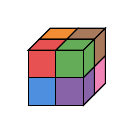
\begin{tikzpicture}[baseline={([yshift=-.5ex]current bounding box.center)}, scale=0.35, z={(0.4,0.4)}]

				% --- Back slice (k=2) ---
				% Top faces (Orange, Brown)
				\draw[fill=cOrange] (0,2,1) -- (1,2,1) -- (1,2,2) -- (0,2,2) -- cycle;
				\draw[fill=cBrown]  (1,2,1) -- (2,2,1) -- (2,2,2) -- (1,2,2) -- cycle;

				% Right faces (Brown, Pink)
				\draw[fill=cBrown]  (2,1,1) -- (2,2,1) -- (2,2,2) -- (2,1,2) -- cycle;
				\draw[fill=cPink]   (2,0,1) -- (2,1,1) -- (2,1,2) -- (2,0,2) -- cycle;

				% --- Front slice (k=1) ---
				% Top faces (Red, Green)
				\draw[fill=cRed]    (0,2,0) -- (1,2,0) -- (1,2,1) -- (0,2,1) -- cycle;
				\draw[fill=cGreen]  (1,2,0) -- (2,2,0) -- (2,2,1) -- (1,2,1) -- cycle;

				% Right faces (Green, Purple)
				\draw[fill=cGreen]  (2,1,0) -- (2,2,0) -- (2,2,1) -- (2,1,1) -- cycle;
				\draw[fill=cPurple] (2,0,0) -- (2,1,0) -- (2,1,1) -- (2,0,1) -- cycle;

				% Front faces (Blue, Purple, Red, Green)
				\draw[fill=cBlue]   (0,0,0) -- (1,0,0) -- (1,1,0) -- (0,1,0) -- cycle;
				\draw[fill=cPurple] (1,0,0) -- (2,0,0) -- (2,1,0) -- (1,1,0) -- cycle;
				\draw[fill=cRed]    (0,1,0) -- (1,1,0) -- (1,2,0) -- (0,2,0) -- cycle;
				\draw[fill=cGreen]  (1,1,0) -- (2,1,0) -- (2,2,0) -- (1,2,0) -- cycle;

			\end{tikzpicture}
			                   & \mapsto
			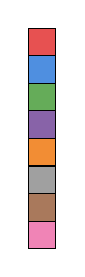
\begin{tikzpicture}[baseline={([yshift=-.5ex]current bounding box.center)}, scale=0.35]
				% Draw the vectorized column from bottom (y=0) to top (y=8)
				\draw[fill=cPink]   (0,0) rectangle (1,1);
				\draw[fill=cBrown]  (0,1) rectangle (1,2);
				\draw[fill=cGrey]   (0,2) rectangle (1,3);
				\draw[fill=cOrange] (0,3) rectangle (1,4);
				\draw[fill=cPurple] (0,4) rectangle (1,5);
				\draw[fill=cGreen]  (0,5) rectangle (1,6);
				\draw[fill=cBlue]   (0,6) rectangle (1,7);
				\draw[fill=cRed]    (0,7) rectangle (1,8);
			\end{tikzpicture}
		\end{aligned}
	\end{equation*}
	dove $ x_l = T(\L^{-1}(l;\miwc[n])) $.
\end{definition}
\begin{remark}
	L'operatore di trasposizione per matrici induce l'ordinamento inverso sulla vettorizzazione.
	Consideriamo ad esempio il caso $ 2\times 2 $:
	\begin{equation*}
		A = \begin{bmatrix} a_{11} & a_{12} \\ a_{21} & a_{22} \end{bmatrix}, \quad A^{\top} =
		\begin{bmatrix} a_{11} & a_{21} \\ a_{12} & a_{22} \end{bmatrix}
		\implies
		\Vec(A) = \begin{bmatrix} a_{11}\\a_{21}\\a_{12}\\a_{22} \end{bmatrix},  \quad \Vec(A^{\top}) =
		\begin{bmatrix} a_{11}\\a_{12}\\a_{21}\\a_{22} \end{bmatrix}.
	\end{equation*}
	Nel caso matriciale si usa riferirsi all'ordine naturale come \emph{column-major} e a quello
	inverso come \emph{row-major}, specialmente nel contesto dei linguaggi di programmazione.
	\todo{Check}
\end{remark}




\section{La fattorizzazione CP}
\label{sec:cp_factorization}

Introduciamo una scrittura di un tensore in tensori elementari, utile a risolvere i seguenti
problemi che affronteremo nei prossimi capitoli.

\textbf{Il problema inverso del rango:} Dato un intero positivo $ r $, nel caso matriciale è, in
linea teorica, un problema semplice costruire una matrice di
rango $ r $; mentre dal punto di vista computazionale, esistono algoritmi polinomiali per
approssimare il rango. Nel caso dei tensori, il problema è difficile su entrambi i fronti. Nella
teoria, trovare un tensore di un certo rango è come trovare un ago in un pagliaio; nella pratica,
approssimare il tensore, o il rango, è numericamente difficile. Questo complica la risoluzione di molti problemi che possono essere modellati tramite tensori, come
vedremo ad esempio nel
Capitolo~\ref{chp:matmul}.

\textbf{Risparmio computazionale:} Cerchiamo una decomposizione di rango basso di un tensore $ T \in \Rmsiz! $ per ridurre il
costo di rappresentazione in memoria e delle operazioni algebriche che lo convolgono. Nel caso matriciale, data una
matrice $ X \in \R^{n_1\times n_2} $ di rango $ r $, possiamo scrivere
\[
	X = UV^{\top} = \begin{bmatrix}  u_1 | \cdots | u_r  \end{bmatrix}  \left[ v_1 | \cdots | v_r \right]^{\top} =
	u_1v_1^{\top} + \cdots + u_rv_r^{\top} = u_1 \topp v_1 + \cdots + u_r \topp v_r
	,\] per certe matrici $ U \in \R^{n_1 \times r} $ e $ V \in \R^{n_2\times r} $. Questo tipo di
decomposizione è vantaggioso in termini di memoria: infatti
\[
	\Vec(X) = v_1 \krn u_1 + \cdots + v_r \krn u_r
	,\] quindi memorizzare $ U $ e $ V $ costa $ O((n_1+n_2)r) $ invece che $ O(n_1n_2) $. Vorremmo
quindi riadattare questa decomposizione per memorizzare $ T $ con costo $ O((n_1+\cdots+n_d)r)
$ invece che $ O(n_1\cdots n_d) $. \todo{discorso unicità} Tuttavia, generalizzare questa decomposizione a più dimensioni ha
numerosi ostacoli \todo{ref to ostacoli}.

\begin{definition}[Canonical Polyadic Decomposition (CP)]
	\label{def:CP}
	Dati degli spazi vettoriali $ A_1 \otimes \cdots \otimes A_d $ e dei vettori $ \{u_1^t, \ldots,
		u_{n_{t}}^t\} \subset A_{t}  $, diciamo che un tensore $ T \in A_1 \otimes \cdots \otimes A_d $
	ammette una \emph{decomposizione CP} di rango $ r \in \N $ se si può scrivere come
	\begin{equation*}
		T = u_1^1 \otimes u_1^2 \otimes \cdots \otimes u_1^d + \cdots + u_r^1 \otimes u_r^2 \otimes \cdots
		\otimes u_r^d.
	\end{equation*}
	\todo{serve ipotesi sui vettori?}
\end{definition}
\begin{remark}
	Siccome $ A_1 \otimes \cdots \otimes A_{n} $ è generato da elementi di rango uno, è sempre
	possibile decomporre un tensore in formato $ CP $.
\end{remark}

\begin{remark}[Canonical Polyadic Decomposition (CP)]
	La decomposizione CP in $ \Rmsiz $ è data da delle matrici $ U_1, \ldots, U_d $ tali che $ U_t = \left[ u_1^t \mid
			\ldots \mid u_r^t\right]\in \R^{n_t \times r} $ tali per cui
	\begin{equation*}
		T = u_1^1 \otimes u_1^2 \otimes \cdots \otimes u_1^d + \cdots + u_r^1 \otimes u_r^2 \otimes \cdots
		\otimes u_r^d \in \Rmsiz.
	\end{equation*}
	In tal caso, scriveremo $ T = \dsqr{U_1, \ldots, U_d} $.
\end{remark}
\begin{remark}
	Possiamo riferirci alla CP sia come decomposizine (data dalla somma dei termini di rango uno)
	oppure come fattorizzazione (data dai fattori $ U_1, \ldots, U_{d} $).
\end{remark}

\begin{remark}
	Fissando la notazione sopra, la fattorizzazione CP si può scrivere nelle seguenti formulazioni equivalenti:
	\begin{enumerate}[label=(\roman*)]
		\item $ T = \sum_{j=1}^r u_j^1 \topp \cdots \topp u_j^d$.
		\item $ \Vec(T) = \sum_{j=1}^r u_j^d \krn \cdots \krn u_j^1$.
		\item $T_{\miwc} = \sum_{j=1}^r U_1(i_1,j)U_2(i_2,j)\cdots U_d(i_d,j)$.
	\end{enumerate}
	\todo{la 3 non torna}
\end{remark}




\begin{figure}[ht]
	\centering
	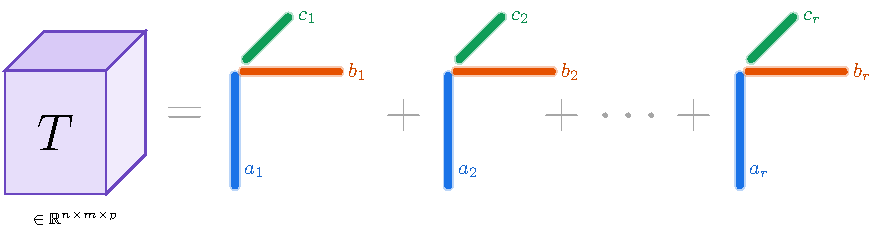
\includegraphics[width=\textwidth, keepaspectratio]{Sources/Chapter1/figures/cp.pdf}
	\caption{Fattorizzazione CP di un tensore $ T = \dsqr{A,B,C} \in \R^{n\times m\times p} $,
		dove i vettori $ a_l,b_l,c_l $ indicano le colonne $ l- $esime di $ A,B,C $.}
	\label{fig:cp_dec}
\end{figure}

\begin{remark}[Risparmio in memoria della CP]
	La fattorizzazione CP di un tensore $ T $ di rango $ r $ permette di ridurre notevolmente il
	costo di memorizzazione, in quanto richiede $ O((n_1 + \ldots + n_d)r) \ll
		O(\prod_{i=1}^d n_j)$.
\end{remark}


\section{Slices, fibers e unfoldings}
\todo{Cambiare}



\begin{definition}[Tensor slice]
	Dato $ T \in \Rmsiz $ chiamiamo \emph{slice (o fetta)} di $ T $ ogni matrice ottenuta da $
		T $ fissando tutti gli indici tranne due. Le slices ottenute fissando gli ultimi $ d-2 $ indici sono dette frontal slices.
	Nel caso $ d=3 $ si identificano tutte le possibili slices (Figura~\ref{fig:tensor_slices}):
	\begin{figure}[htbp]
		\centering
		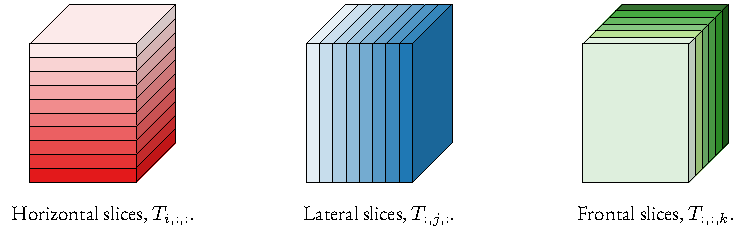
\includegraphics[width=\textwidth, keepaspectratio]{Sources/Chapter1/figures/slices.pdf}
		\caption{Slices di un tensore di ordine 3: fette orizzontali $X_{i::}$ (mode-1), laterali $X_{:j:}$ (mode-2) e frontali $X_{::k}$ (mode-3).}
		\label{fig:tensor_slices}
	\end{figure}
\end{definition}

\begin{definition}[Mode-$k$ fiber]
	Dato un tensore $ T \in \Rmsiz!$ chiamiamo \emph{fibers} i vettori ottenuti fissando
	tutti gli indici tranne uno. Quando l'indice libero di variare è il $ k $-esimo lo chiamiamo
	\emph{mode-$k$ fiber}. Nel caso $ d=3 $ denotiamo le fibre come fibre colonna $x_{:jk}$ (mode-1), fibre riga $x_{i:k}$ (mode-2) e fibre tubo $x_{ij:}$ (mode-3), come illustrato in Figura~\ref{fig:tensor_fibers}.
	\begin{figure}[htbp]
		\centering
		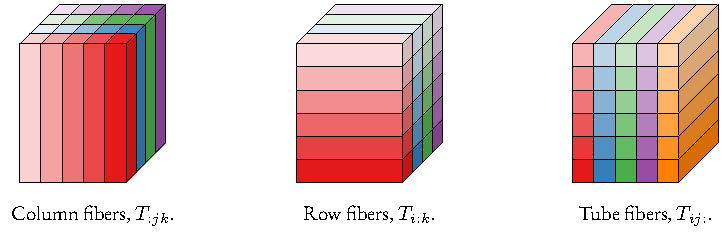
\includegraphics[width=\textwidth, keepaspectratio]{Sources/Chapter1/figures/fibers.pdf}
		\caption{Fibre di un tensore di ordine 3: fibre colonna $x_{:jk}$ (mode-1), riga $x_{i:k}$ (mode-2) e tubo $x_{ij:}$ (mode-3).}
		\label{fig:tensor_fibers}
	\end{figure}
\end{definition}

In molte situazioni risulta comodo disporre gli elementi di un tensore in una matrice. Uno dei modi
per farlo è utilizzare le matricizzazioni, anche dette \emph{unfoldings}.

\begin{definition}[Mode-$k$ unfolding]
	Il \emph{mode-$k$ unfolding} di un tensore $ T \in \Rmsiz! $ è la matrice $ \Tm{T}{k} \in \R^{n_k \times
			\prod_{j\neq k}n_j} $ le cui colonne sono mode-$ k $ fibers ordinate seguendo l'ordine naturale
	su $ \sdom $. In particolare si ha
	\[
		(\Tm{T}{k})_{i,j} = T_{\siwc{i}} \text{, con } j = \L(\siwc)
		.\]
\end{definition}
\begin{remark}
	Possiamo pensare all'unfolding nel modo $ k $ come a rimappare l'indice $ i_{k} $ sulle righe e
	l'indice $ (i_1, \ldots, i_{k-1}, i_{k+1}, \ldots, i_{d}) $ sulle colonne.
\end{remark}

\begin{figure}[htbp]
	\centering
	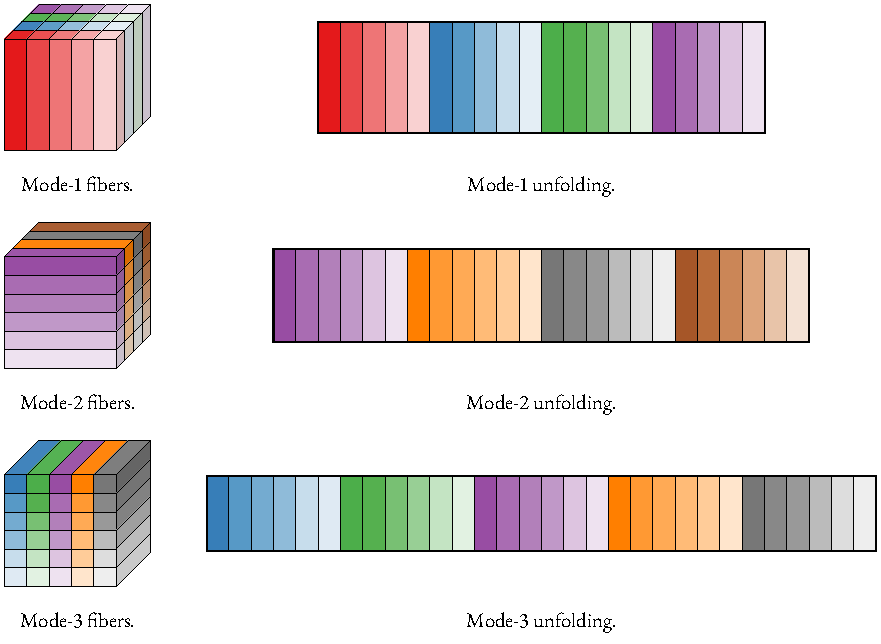
\includegraphics[width=\textwidth, keepaspectratio]{Sources/Chapter1/figures/fibers_unfolding.pdf}
	\caption{Fibre e matricizzazioni nei tre modi per un tensore del terzo ordine.}
	\label{fig:fibers_unfolding}
\end{figure}

\begin{example}[De Lathauwer~\cite{lieven2006}]
	Consideriamo il tensore $ T $ di taglia $ 2\times 2\times 2 $ definito da
	\begin{equation*}
		a_{111}=-a_{121} = 3, \quad a_{211} = -a_{221} = 6, \quad a_{112} = -a_{122} = 1, \quad a_{212} = - a_{222} = 2.
	\end{equation*}
	I vettori dei modi $ 1,2 $ e $ 3 $ sono le colonne delle matrici
	\begin{equation*}
		\Tm{T}{1} = \begin{bmatrix} 3 & -3 & 1 & -1 \\ 6 & -6 & 2 & -2 \end{bmatrix}, \quad
		\Tm{T}{2} = \begin{bmatrix} 3 & 6 & 1 & 2 \\ -3 & -6 & -1 & -2 \end{bmatrix}, \quad
		\Tm{T}{3} = \begin{bmatrix} 3 & 6 & -3 & -6 \\ 1 & 2 & -1 & -2 \end{bmatrix},
	\end{equation*}
	rispettivamente. Il tensore ha rango uno perché si può decomporre come
	\begin{equation*}
		T = \begin{bmatrix} 1 \\ 2 \end{bmatrix}  \topp \begin{bmatrix} 1 \\ -1 \end{bmatrix} \topp
		\begin{bmatrix} 3 \\ 1 \end{bmatrix}.
	\end{equation*}
	Pensando la terza dimensione nel verso entrante al foglio, possiamo riassumere i passaggi svolti
	per fattorizzare $ T $, dove è stata applicata più volte la definizione di prodotto tensore:
	\todo{c'è un typo!}
	\begin{center}
		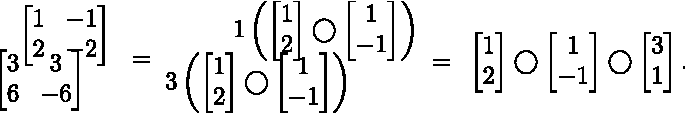
\includegraphics[width=0.65\textwidth, keepaspectratio]{./Sources/Chapter1/figures/cp_example.pdf}
	\end{center}
\end{example}

\begin{figure}[htbp]
	\centering
	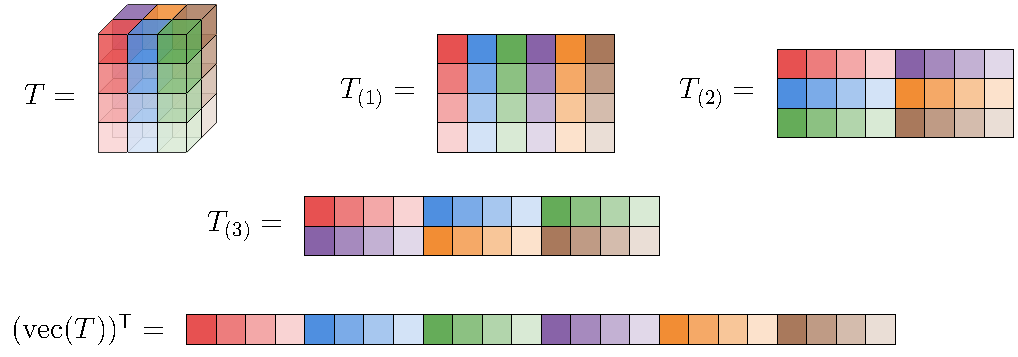
\includegraphics[width=\textwidth, keepaspectratio]{Sources/Chapter1/figures/unfoldings.pdf}
	\caption{Schema delle matricizzazioni e vettorizzazione di un tensore.}
	\label{fig:unfoldings}
\end{figure}
L'operazione di unfolding permette anche di catturare il suo rango (matriciale) lungo ogni direzione:

\todo{anche def landsberg}
\begin{definition}[Rango multilineare]
	Il \emph{rango multilineare} o \emph{multirank} di un tensore $ T \in \Rmsiz $ è la $ d $-upla $
		(r_1, r_2, \ldots, r_d) $, dove $ r_k = \rank{\Tm{T}{k}} $, per ogni $ k \in \{1, \ldots, d\}
	$. Lo denotiamo con $ \multirk(T) $.
\end{definition}


Dal punto di vista computazionale è utile introdurre la seguente operazione

\todo{refrasare un poco per renderla più leggibile}
\begin{definition}[Reshape]
	Definiamo l'operatore di \emph{reshape} come l'operazione riarrangia il tensore senza alterarne le dimensioni e mantenendo l'ordine delle entrate. Formalmente,
	fissati $ d, d' \in \N$ e un tensore $ T \in \Rmsiz! $, per ogni $ m_1, \ldots, m_{d'} $ tali
	che $ \prod_{i=1}^{d'} m_j = \prod_{j = 1}^{d} n_j$, il tensore $ \Tn{y} = \reshape(T,
		\msiz![m][d']) \in \Rmsiz![m][d'] $ è definito come
	\[
		\Tn{y}(i_1, \ldots, i_{d'})= T(j_1, \ldots, j_d)
		,\]
	per ogni $(i_1, \ldots, i_{d'}),(j_1, \ldots,
		j_d) $ tali che $ \L(i_1, \ldots, i_{d'}; \msiz![m][d'])) = \L(j_1, \ldots,
		j_d; \msiz!)$.
\end{definition}
\begin{remark}
	Un reshape ha costo nullo perché non si spostano celle di memoria, ma si eseguono solo operazioni
	di indici. Questa proprietà vale in particolare per tutte le strutture dati (vettori, matrici,
	tensori) $ \tilde{T} $ tali che $ \vec(\tilde{T}) = \vec(T) $.
\end{remark}
\begin{remark}
	L'unfolding sul primo modo ha costo nullo, in quanto $ \Tm{T}{1} = \reshape(T, n_1 \times
		\prod_{j=2}^d n_{j}) $, cioè
	\begin{equation*}
		\Tm{T}{1} = \left[\begin{array}{c|c|c}
				T_{:, \ldots, :,1} & \dots & T_{:, \ldots, :, n_{d}}
			\end{array}\right] \in \R^{n_1 \times
			\prod_{j=2}^d n_{j}}.
	\end{equation*}
\end{remark}
\begin{remark}
	Per $ k>1 $, formare l'unfolding $ \Tm{T}{k} $ ha un costo non banale, in particolare $
		\vec(\Tm{T}{k}) \neq \vec(T) $.

	Se $ k=d $, l'unfolding $ \Tm{T}{d} = \begin{bmatrix} \vec(T_{:, \ldots, :, 1})^{\top} \\  \vdots
			\\ \vec(T_{:, \ldots, :, n_{d}})^{\top}\end{bmatrix}  $, e in particolare vale $
		\vec(\Tm{T}{d}^{\top}) = \vec(T)$. Quindi calcolare la trasposta dell'ultimo unfolding
	non costa nulla.
\end{remark}

\begin{lemma}[Vettorizzazione e unfolding di un tensore di rango uno]
	\label{lhm:vec_unf_rk1}
	Dato un tensore $ T = v^1 \topp \cdots \topp v^d $, allora
	\begin{enumerate}[label=(\roman*)]
		\item $\Vec(T) = v^d \krn \cdots \krn v^1$.
		\item $ \Tm{T}{k} = v^k\left( v^d \krn \cdots \krn v^{k-1} \krn v^{k+1} \krn \cdots
			      \krn v^1 \right)^{\top}$.
	\end{enumerate}
	In particolare, tutte le matricizzazioni di un prodotto esterno hanno rango 1.
\end{lemma}
\begin{proof}
	La $ (i) $ segue applicando più volte l'Osservazione~\ref{rmk:krn_tensor}. Dimostriamo la $ (ii)
	$. Per definizione di tensore di rango uno~\eqref{eq:rk1_components} la scrittura in componenti di $ T $ è
	\begin{equation*}
		T_{i_1, \ldots, i_{d}} = v^1_{i_1} \cdots v^d_{i_{d}} = v^k_{i_{k}} \left( \prod_{\substack{m=1
				\\ m\neq k}}^d v^m_{i_{m}}\right).
	\end{equation*}
	Preso $ u = v^d \krn \cdots \krn v^{k+1} \krn v^{k-1} \krn \cdots \krn v^1 $, osserviamo che la
	sua componente $ j $-esima è il prodotto fra parentesi, ovvero $ u_{j} =\left( \prod_{\substack{m=1
				\\ m\neq k}}^d v^m_{i_{m}}\right) $. A questo punto, per definizione di unfolding abbiamo
	$ \left( \Tm{T}{k} \right)_{i_{k},j} = v^k_{i_{k}}u_{j}$, da cui
	\begin{equation*}
		\Tm{T}{k} = v^k u^{\top} = v^k \left( v^d \krn \cdots \krn v^{k+1} \krn v^{k-1} \krn \cdots \krn
		v^1 \right)^{\top}.
	\end{equation*}
\end{proof}

In molte situazioni è utile moltiplicare un tensore con una matrice, ma purtroppo le dimensioni non
combaciano. La seguente definizione risolve
il problema facendo agire la matrice la matrice lungo il modo $ k- $esimo di un tensore, e si
chiama.
\begin{definition}[Prodotto nel modo $k$]
	Il \emph{prodotto nel modo $ k $} di un tensore $ T \in \Rmsiz! $ con una matrice $ U \in
		\R^{r \times n_k} $ descrive l'azione di $ U $ sulla $ k $-esima coordinata di $ T $. Formalmente, è un tensore
	\[
		Y = T \ttm U \in \R^{\ssiz{r}} \text{ con } \Tm{Y}{k} = U \Tm{T}{k}
		.\]
	In componenti, $ Y_{\siwc{\alpha}} = \sum_{i_k = 1}^d T(\miwc) U_{\alpha, i_k} $.
\end{definition}


\todo{Esempio polinomio semisep + altro es}


\section{Il problema del rango}
\label{sec:cp_rank}

In più dimensioni il problema di calcolare il rango, e una fattorizzazione CP di un tensore si
complicano notevolmente rispetto al caso matriciale.\todo{non mi piace}
Ci sono molte domande aperte riguardo al rango, ad esempio non si ha una risposta generale (a
differenza del
caso matriciale) a domande del tipo:
\begin{enumerate}
	\item Qual'è il massimo rango possibile per un tensore di dimensione $ n_1 \times \cdots \times n_d $?
	\item Quali sono i ranghi \emph{tipici}, ovvero quelli ottenuti con probabilità non nulla quando si genera un tensore di entrate casuali?
\end{enumerate}
Per capire il motivo, discutiamo alcune caratteristiche dei tensori che rendono complesso il ``problema del
rango''.

\subsection*{Border rank}
Nel caso delle matrici, una successione di matrici di rango $ r $ converge sempre a una matrice di
rango $ \le r $. Per i tensori possono accadere dei ``salti'', in altre parole, la varietà dei
tensori di un rango fissato $ r $ non è chiusa\footnote{Non precisiamo la topologia, per una
	discussione formale si vedano~\cite{landsberg2011tensors,landsberg2015geometry}.}, ad esempio, un tensore di rango $ 2 $
può convergere ad uno di rango $ 3 $, come mostra il prossimo esempio. Questo inconveniente teorico
ha risvolti interessanti che vedremo nella \S~\ref{sec:APA}.

\begin{example}
	\label{ex:border_rank}
	Consideriamo dei vettori $ a_1,a_2 \in \R^m$, $b_1,b_2 \in \R^n$ e $c_1,c_2\in \R^p $ vettori
	linearmente indipendenti. Definiamo il tensore
	\begin{equation}
		T = a_1 \topp  b_1 \topp c_2 + a_1 \topp b_2 \topp c_1 + a_2 \topp b_1 \topp c_1,
	\end{equation}
	e notiamo che $ \rk(T) = 3 $ dato che non può
	essere scomposto come somma di tensori più semplici.
	Consideriamo la successioni di tensori
	\begin{equation}
		\label{eq:rank_counterex}
		T_\varepsilon = \frac{1}{\varepsilon}\left( a_1 +
		\varepsilon a_2 \right) \topp (b_1 + \varepsilon b_2) \topp (c_1 + \varepsilon c_2) -
		\frac{1}{\varepsilon} a_1 \topp b_1 \topp c_1, \text{ con } \varepsilon \in \R,
	\end{equation}
	che essendo combinazione lineare di due tensori di rango uno, ha rango 2.
	Vediamo che $ \lim_{\varepsilon \to 0} T_\varepsilon = T $, da cui segue che l'insieme dei tensori di rango 3 non è chiuso.
	Espandendo i termini dell'Equazione \eqref{eq:rank_counterex} tramite la proprietà distributiva del prodotto esterno,
	\begin{equation}
		\begin{aligned}
			\Tn{y}_\varepsilon & =  \frac{1}{\varepsilon} a_1 \topp b_1 \topp c_2 + a_1 \topp b_1 \topp c_2 + a_1 \topp b_2 \topp c_1
			+a_2 \topp b_1 \topp c_1                                                                                                  \\ &+ \varepsilon \left(a_2 \topp b_2 \topp c_1 + a_1 \topp b_1 \topp c_2 +
			a_1 \topp b_2 \topp c_2 + a_2 \topp b_2 \topp c_2 \right) - \frac{1}{\varepsilon} a_1 \topp
			b_1 \topp c_1                                                                                                             \\
			                   & = T + \varepsilon\left(a_2 \topp b_2 \topp c_1 + a_1 \topp b_1 \topp c_2 +
			a_1 \topp b_2 \topp c_2 + a_2 \topp b_2 \topp c_2 \right)
		\end{aligned}
	\end{equation}
	Quindi $ T_\varepsilon - T \to 0 $.
\end{example}

Questo motiva la seguente definizione:


\begin{definition}[Border rank]
	Un tensore $ T $ ha \emph{border rank} $ r $ se è limite di una successione di tensori di
	rango $ r $, ma non è limite di una successione di tesori di rango $ s $, per ogni $ s < r $. Lo
	denoteremo con il simbolo $ \brk(T) $.
\end{definition}
\begin{remark}
	$ \rk(T) \ge \brk(T) $.
\end{remark}
\begin{remark}
	In altri termini, se $ T \in \Rmsiz $, il suo border rank è la quantità
	\[
		\brk(T) = \min \left\{ r \in \N \mid \exists T' \in \Rmsiz! \text{ tale che }
		\rk(T')=r, \, \|T - T'\|  < \varepsilon \right\}
		.\]
\end{remark}
\todo{Disegno interpretazione geometrica (landsberg pg 38)}

Il border rank ammette anche la seguente interpretazione geometrica:




\subsection*{Costo computazionale}
\label{sec:computing_rank}
Calcolare il costo di una fattorizzazione CP usando un algoritmo esatto è NP-Hard~\cite{haastad1989tensor}. Non
solo; il problema di trovare un tensore approssimante di un certo rango è computazionalmente
difficile. In altre parole, la miglior approssimazione di rango $ r $ è data da dei vettori $ x_{i}
	\in \R^{n_1}, y_{i} \in \R^{n_2}, \ldots, z_{i} \in \R^{n_{d}}   $, per $ i = 1, \ldots, r $ che minimizzano
\begin{equation*}
	\| A - x_1 \otimes y_1 \otimes \cdots \otimes z_1 - \cdots x_{r} \otimes y_{r} \otimes \cdots
	\otimes z_{r}\|
\end{equation*}
oppure, in altre parole un tensore $ B $ dato da una fattorizzazione CP, che realizza
\begin{equation*}
	\min_{\rank(B) \le r} \| A - B \|.
\end{equation*}
Qui $ \| \cdot \| $ denota una norma fissata su $ \R^{n_1 \times  \cdots \times n_{d}}$. Quando $ d =2$, il
problema è risolto per norme invarianti per trasformazioni unitarie su $ \R^{m \times n} $ dal
teorema di Eckart-Young-Mirsky~\cite{eckart1936approximation}: se
\begin{equation*}
	A = U\Sigma V^* = \sum_{i = 1}^{\rank(A)}\sigma_i u_{i} \otimes v_{i}, \qquad \sigma_{i} \ge
	\sigma_{i+1},
\end{equation*}
è la decomposizione ai valori singolari di $ A $ (anche detta SVD), allora la migliore
approssimazione di rango $ r $ è data dai primi $ r $ termini della somma.
Sfortunatamente, generalizzare questo risultato in più dimensioni è
ritenuto molto difficile (o impossibile)~\cite{desilva2008tensorrankillposednessbest}.

Nella pratica esistono diverse euristiche per calcolare il rango. Una di queste è scegliere come rango il più piccolo $ r $ che minimizza l'errore
relativo rispetto al rango $ r-1 $. Per un tensore a $ 3 $ indici, l'\emph{errore relativo} è
definito in questo modo:
\begin{equation}
	\label{eq:rel_error}
	\varepsilon_{\text{rel}} = \frac{\| T - \dsqr{A,B,C} \|}{\|T\|} = \frac{\left(\sum_{i,j,k}\left( t_{ijk} -
		\sum_{l=1}^r a_{il}b_{jl}c_{kl}\right)^2 \right)^{\frac{1}{2}}}{\left( \sum_{i,j,k}
		t_{ijk}
		\right)^{\frac{1}{2}}}.
\end{equation}

\subsection*{Rango massimo}

Nel caso di una matrice $ m \times n $, il suo rango massimo è $ \min \{m,n\}  $. Per un tensore, il
\emph{rango massimo} è definito come il massimo dei ranghi realizzabili per dei tensori $ T \in
	\R^{n_1 \times \cdots \times n_{d}} $ di una certa taglia fissata. In altre parole,
\begin{equation*}
	\rk_{\text{max}}(\R^{n_1\times n_2 \times \cdots \times  n_{d}}) = \max \{ \rk(T) \mid T \in
	\R^{n_1 \times n_2 \times \cdots \times n_{d}}\}.
\end{equation*}
Sfortunatamente, ad eccezione di alcuni casi speciali, i ranghi massimi per la maggior parte dei
tensori di ordine superiore sono sconosciuti. I casi speciali in cui il rango massimo è noto sono elencati nella Tabella~\ref{tab:max_ranks}. Il primo risultato per tensori di dimensione $2 \times m \times n$ implica, ad esempio, che un tensore di taglia $2 \times 2 \times 2$ ha un rango massimo pari a $3$.

\begin{table}[htbp]
	\centering
	\small
	\caption{Ranghi massimi tensoriali noti. L'ordine delle dimensioni non modifica il rango, quindi le taglie sono ordinate dalla più piccola alla più grande (tratta da Ballard e Kolda~\cite[Tabella~16.1]{BK25}).}
	\label{tab:max_ranks}
	\begin{tabular}{lll}
		\toprule
		Taglia tensore                     & Rango massimo                           & Fonte                                            \\
		\midrule
		$2 \times m \times n \; (m \le n)$ & $m + \min \{ m, \lfloor n/2 \rfloor \}$ & JáJá~\cite{jaja1979}; Kruskal~\cite{kruskal1989} \\
		$3 \times 3 \times 3$              & $5$                                     & Kruskal~\cite{kruskal1989}                       \\
		$3 \times 7 \times 7$              & $8$                                     & Atkinson e Stephens~\cite{atkinson1979}          \\
		$2 \times 4 \times 4$              & $6$                                     & ten Berge~\cite{tenberge2000b}                   \\
		\bottomrule
	\end{tabular}
\end{table}

È inoltre possibile derivare un limite superiore debole per il rango massimo:
\todo{se lasci verificalo}
\begin{equation}
	\label{eq:weak_upper_bound_max_rank}
	\rk_{\text{max}}(\R^{n_1 \times n_2 \times \cdots \times n_d}) \le \min_k \prod_{\substack{\ell=1 \\ \ell \neq k}}^d n_\ell = \frac{\prod_{k=1}^d n_k}{\max_k n_k}.
\end{equation}



\subsection*{Rango tipico}
\label{sec:rango_tipico}

Mentre le matrici random hanno rango massimo con probabilità uno\footnote{L'idea è presa una matrice
	con entrate estratte da una distribuzione di probabilità continua, il
	determinante è un polinomio le cui indeterminate sono le entrate della matrice. Il luogo di
	zeri di questo polinomio ha misura di Lebesgue nulla, quindi integrando la densità di probabilità
	sul luogo di zeri dà probabilità nulla. La tesi si ha passando al compolementare.}, per un tensore di un
formato fissato potrebbe esserci più di un rango con probabilità positiva. Questo fenomeno è noto
come \emph{rango tipico}.

Sia $ \mathcal{D}(n_1, n_2, \ldots, n_{d})$ una distribuzione di probabilità continua sullo spazio
dei tensori $ \R^{n_1 \times n_2 \times \cdots \times n_{d}} $ (un esempio sono i tensori a entrate
gaussiane).
\begin{definition}
	Il \emph{rango tipico} (o \emph{rango generico}) di un tensore $ T \in \K^{n_1 \times \cdots
			\times n_{d}} $ è l'insieme dei ranghi che occorrono con probabilità non nulla, rispetto ad
	ogni distribuzione continua $  \mathcal{D}(n_1, n_2, \ldots, n_{d})$ sull'insieme di tali tensori.
	In formule,
	\begin{equation*}
		\rk_{\text{typical}} = \{r \mid P \left( \rk(T) = r, \; T \sim \mathcal{D}(n_1, \ldots,
			n_{d})\right) > 0\}.
	\end{equation*}
\end{definition}

\todo{rewrite and verify}

Mentre per le matrici il rango tipico è unico e coincide con il massimo rango possibile, per i
tensori di ordine superiore a due. In particolare su $\mathbb{R}$ possono coesistere
più ranghi tipici, mentre su $\mathbb{C}$ il rango tipico è sempre unico. La Tabella~\ref{tab:typical_ranks} riassume i principali risultati noti in letteratura, tratti da Ballard e Kolda~\cite[p.~276, Tabella~16.2]{BK25}.
Per verificare questi risultati, abbiamo implementato un esperimento numerico.
Selezionando alcuni formati, abbiamo generato dei tensori casuali con entrate estratte
indipendentemente sia da una distribuzione normale standard $\mathcal{N}(0, 1)$ sia da una
distribuzione uniforme $\mathcal{U}(-1, 1)$. Il rango di ciascun tensore è stato stimato
usando l'algoritmo ALS\todo{ref} su un campione di $ 200 $ tensori, facendo $ 120 $ restarts e un
numero massimo di $ 500 $ iterazioni, interrompendo una volta raggiunto un errore relativo inferiore a
$10^{-5}$. La distribuzione empirica dei ranghi riportata in Figura~\ref{fig:typical_ranks_dist} mostra che la
distribuzione delle entrate (normale o uniforme) non altera l'insieme dei ranghi tipici e produce frequenze empiriche analoghe.

\begin{figure}[htbp]
	\centering
	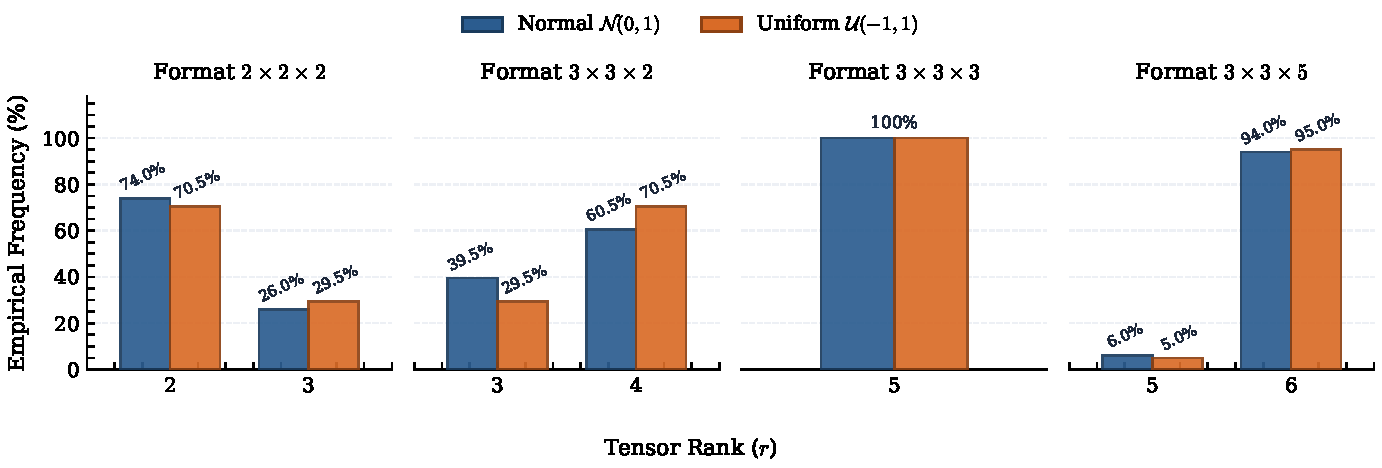
\includegraphics[width=\textwidth, keepaspectratio]{Sources/Chapter1/figures/typical_rank_distribution.pdf}
	\caption{Distribuzione empirica dei ranghi per tensori casuali reali di formato $2 \times 2 \times 2$, $3 \times 3 \times 2$, $3 \times 3 \times 3$ e $3 \times 3 \times 5$ con entrate estratte da distribuzioni Normali $\mathcal{N}(0, 1)$ ed Uniformi $\mathcal{U}(-1, 1)$ (istogrammi affiancati).}
	\label{fig:typical_ranks_dist}
\end{figure}

\begin{table}[htbp]
	\centering
	\small
	\caption{Ranghi tipici noti sul campo reale $\mathbb{R}$ per tensori di dimensione $m \times n \times p$ con $2 \le m \le n \le p$ (adattata da Ballard e Kolda~\cite[Tabella~16.2]{BK25}).}
	\label{tab:typical_ranks}
	\begin{tabular}{lll}
		\toprule
		Formato ($m \times n \times p$)                   & Rango tipico & Fonte                                                                \\
		\midrule
		$2 \times n \times n$                             & $\{n, n+1\}$ & ten Berge, Kiers~\cite{tenberge1999}                                 \\
		$3 \times 3 \times 3$                             & $5$          & ten Berge, Stegeman~\cite{tenberge2006}                              \\
		$3 \times 3 \times 5$                             & $\{5, 6\}$   & ten Berge, Sidiropoulos, Rocci~\cite{tenberge2004}                   \\
		$3 \times 4 \times 8$                             & $\{8, 9\}$   & Sumi et al.~\cite{sumi2013}                                          \\
		$3 \times 5 \times 9$                             & $\{9, 10\}$  & Choulakian~\cite{choulakian2010}; ten Berge~\cite{tenberge2011}      \\
		$4 \times 4 \times 12$                            & $\{12, 13\}$ & Friedland~\cite{friedland2012}                                       \\
		$m \times n \times n(m-1)$ ($m > 2$, $n$ dispari) & $n(m-1)$     & ten Berge~\cite{tenberge2000b}                                       \\
		$m \times n \times p$ ($n(m-1) < p < mn$)         & $p$          & ten Berge, Kiers~\cite{tenberge1999}; ten Berge~\cite{tenberge2000b} \\
		$m \times n \times p$ ($p \ge mn$)                & $mn$         & ten Berge, Kiers~\cite{tenberge1999}; ten
		Berge~\cite{tenberge2000b}                                                                                                              \\
		\bottomrule
	\end{tabular}
\end{table}


\subsection*{Dipendenza dal campo base}
Nel caso matriciale ogni matrice $ m \times n $ a entrate reali ha lo stesso
rango se visto come elemento di $ \R^{m\times n} $ o di $ \C^{m \times n} $, per i tensori questo è
falso. Consideriamo il seguente esempio:
\begin{example}[De Silva e Lim~\cite{desilva2008tensorrankillposednessbest}]
	Scriviamo $ z_{k} = x_{k} + \I y_{k} $ e $ \overline{z}_k = x_{k} - \I y_{k} $, allora
	\begin{equation}
		\begin{aligned}
			 & \frac{1}{2}\left( \overline{z}_1 \topp z_2 \topp \overline{z}_3 + z_1 \topp \overline{z}_2 \topp
			z_3\right)                                                                                          \\
			 & = x_1 \topp x_2 \topp x_3 + x_1 \topp y_2 \topp y_3 - y_1 \topp x_2 \topp
			y_3 + y_1 \topp y_2 \topp x_3.
		\end{aligned}
	\end{equation}
	Chiamando $ I = \overline{z}_{1} \otimes z_2 \otimes \overline{z}_3 $ e $ II = z_1 \otimes
		\overline{z}_{2} \otimes z_3 $, usando la proprietà distributiva e la trilinearità del prodotto
	tensore,
	\begin{equation*}
		\begin{aligned}
			I  & = (x_1 - \I y_1) \otimes (x_2 + \I y_2) \otimes (x_3 - \I y_3)                              \\
			   & = x_1 \otimes x_2 \otimes x_3 - \I x_1 \otimes x_2 \otimes y_3 + \I x_1 \otimes y_2 \otimes
			x_3                                                                                              \\
			   & + x_1 \otimes y_2 \otimes y_3 - \I y_1 \otimes x_2 \otimes x_3 - y_1 \otimes x_2 \otimes
			y_3                                                                                              \\
			   & + y_1 \otimes y_2 \otimes x_3 - \I y_1 \otimes y_2 \otimes y_3,                             \\
			II & = (x_1 + \I y_1) \otimes (x_2 - \I y_2) \otimes (x_3 + \I y_3)                              \\
			   & =x_1 \otimes x_2 \otimes x_3 + \I x_1 \otimes x_2 \otimes y_3 - \I x_1 \otimes y_2
			\otimes x_3                                                                                      \\
			   & + x_1 \otimes y_2 \otimes y_3 + \I y_1 \otimes x_2 \otimes x_3 - y_1 \otimes x_2 \otimes
			y_3                                                                                              \\
			   & + y_1 \otimes y_2 \otimes x_3 + \I y_1 \otimes y_2 \otimes y_3.
		\end{aligned}
	\end{equation*}
	L'espressione sopra segue calcolando $ \frac{1}{2}(I + II) $.

\end{example}

\section{Il teorema del rango}

Data la complessità del problema del rango possiamo stimarlo rango con la seguente
proposizione, dalla quale intuiamo che non sarà semplice trovare stime del rango di un
tensore---queste spesso coinvolgono tecniche algebrico-combinatoriche avanzate. Vedremo alcuni esempi di
queste stime nella Sezione~\ref{sec:exp_estimates}.

Definiamo un'operazione utile tra le colonne di due matrici, che sarà utile a dimostrare il
risultato di questa sezione.
\begin{definition}[Prodotto Khatri-Rao]
	Date due matrici $ A \in \R^{m \times r} $ e $ B \in \R^{n \times r} $, il loro \emph{prodotto
		Khatri-Rao} è dato da
	\begin{equation}
		C = A \krp B = \left[ a_1 \krn b_1 \mid \ldots \mid a_r \krn b_r \right] \in \R^{(mn) \times r},
	\end{equation}
	dove $ a_j $ e $ b_j $ indicano la $ j$-esima colonna di $ A $ e $ B $, rispettivamente, e la matrice $ C $
	si lascia scrivere in componenti come $ C_{kl} = A_{il}B_{jl} $, dove $ \L^*(i,j) = \L(j,i) = k $.
\end{definition}
\begin{remark}
	\label{rmk:krp_sub_krn}
	Il prodotto $ A \krp B $ è sottomatrice di $ A \krn B $, in quanto una colonna $ k $-esima della
	prima è del tipo $ a_{k} \krn b_{k} $, mentre per la seconda è $ \left[ a_{1k}B, \ldots, a_{mk}B
			\right]^{\top} $; quindi possiamo ottenere la prima matrice selezionando alcune colonne della
	seconda.
\end{remark}
\begin{remark}
	\label{rmk:krp_as_span}
	Data una fattorizzazione $ T = \dsqr{U_1, \ldots, U_{d}}$, il prodotto Khatri-Rao
	\begin{equation*}
		U_{d} \krp U_{d-1} \krp \cdots \krp U_1
	\end{equation*}
	ha come colonna $ r $-esima $ u^d_r \krn u^{d-1}_r \krn \cdots  \krn u^1_r$, in altre parole, è la
	rappresentazione matriciale dell'insieme $ \left\{ u^d_r \krn u^{d-1}_r \krn \cdots  \krn u^1_r\right\}_{r=1,
				\ldots, d} $ formato
	dagli addendi della decomposizione $ \vec(T) = \sum_{r=1}^R u^d_r \krn u^{d-1}_r \krn \cdots  \krn u^1_r $.
	In particolare, vale
	\begin{equation*}
		\begin{aligned}
			\Vec({T}) & = \sum_{h=1}^r u_h^d \krn \cdots \krn u_h^1 = \left[ u_1^d
			\krn \cdots \krn u_1^1 | \cdots | u_r^d \krn \cdots \krn u_r^1\right]^{\top}\mathbf{1}_r \\
			          & = \left( U_d \krp U_{d-1} \krp \cdots \krp U_1 \right) \mathbf{1}_r.
		\end{aligned}
	\end{equation*}

\end{remark}

\begin{remark}
	Calcolare il prodotto di Khatri-Rao di due matrici $ A \in \R^{m \times r} $ e $ B \in \R^{n \times
			r} $ ha un costo in memoria di $ O(mn
		r) $.
\end{remark}

\begin{lemma}
	\label{lhm:krp_unfoldings}
	Data una fattorizzazione $ T = \dsqr{U_1,\ldots, U_d} \in \Rmsiz!$, essa ha come unfoldings
	\[
		\Tm{T}{j} = U_j \left( U_d \krp U_{d-1} \cdots \krp U_{j+1} \krp U_{j-1} \krp \cdots U_1 \right)^{\top}
		,\]  per ogni $ j = 1, \ldots, d $.
\end{lemma}
\begin{proof}
	Scrivendo le matricizzazioni di $ T = \sum_{h=1}^r u_h^1 \topp \cdots \topp u_h^d $, dove i vettori $ u_1^j,
		\ldots, u_r^j $ rappresentano le colonne della matrice $ U_j $, troviamo che
	\begin{equation*}
		\begin{aligned}
			\Tm{T}{j} & = \sum_{h=1}^r u_h^j \left( u_h^d \krn \cdots \krn u_h^{j+1} \krn u_h^{j-1} \krn
			\cdots \krn u_h^1 \right)^{\top}                                                             \\
			          & = U_j \begin{bmatrix} u_1^d \krn \cdots \krn u_1^1 | \cdots | u_r^d \krn \cdots
				                  \krn u_r^1\end{bmatrix}^{\top}   \\
			          & = U_j \left( U_d \krp \cdots \krp U_{j+1} \krp U_{j-1} \krp \cdots \krp U_1
			\right)^{\top},
		\end{aligned}
	\end{equation*}
	dove nel primo passaggio abbiamo applicato la Proposizione~\ref{lhm:vec_unf_rk1} su ogni addendo di rango uno.
\end{proof}
\begin{example}
	Se $ T = \dsqr{A,B,C} $, allora segue che $ \Tm{T}{1} = A \left( C \krp B \right)^{\top} $.
\end{example}




\begin{proposition}[Teorema del rango]
	\label{th:rank}
	Sia $ T \in \Rmsiz! $ un tensore che ammette fattorizzazione $ T = \dsqr{U_1, \ldots,
			U_d} $, e sia $ r_j = \rank(\Tm{T}{j}) $ il rango dell'unfolding $ \Tm{T}{j} $ con $ j = 1, \ldots, d $. Allora vale che
	\begin{equation}
		\max_{j=1, \ldots, d}(r_j) \le \rk(T) \le \min_{j=1, \ldots, d}\left( \prod_{i \neq j}r_i \right)
	\end{equation}
\end{proposition}
\begin{proof}
	Fissato $ r = \rk(T) $, la minorazione segue direttamente dal fatto che ogni unfolding $ \Tm{T}{j}
	$ è una matrice di taglia $ n_{j} \times r  $.
	Mostriamo la maggiorazione, assumendo senza perdita di generalità che $ \rk(T) \le
		\prod_{i=2}^d r_i $. Consideriamo la vettorizzazione
	\begin{equation}
		\label{eq:vec_rk_krn}
		\Vec(T) = \sum_{k=1}^r u_k^d \krn \cdots \krn u_k^2 \krn u_k^1.
	\end{equation}
	Allora l'insieme
	\[
		\left\{u_k^d \krn \cdots \krn u_k^2\right\}_{k = 1, \ldots, r}
	\] è formato da vettori linearmente indipendenti. Se così non fosse,
	esisterebbe un indice $ k_0 $, che possiamo supporre $ k_0 = 1 $ a meno di riordinamento degli
	indici $ k $, tale per cui
	\begin{equation}
		u_{1}^d \krn \cdots \krn u_{1}^2 = \sum_{h = 2}^r c_h(u_h^d \krn \cdots \krn u_h^2),
	\end{equation}
	che sostituita nella Equazione~\eqref{eq:vec_rk_krn} porta alla seguente decomposizione:
	\begin{equation*}
		\begin{aligned}
			\Vec(T) & = \sum_{k=2}^r u_k^d \krn \cdots \krn u_k^2 \krn u_k^1 + \left(\sum_{k=2}^r c_k
			\left(u_k^d \krn \cdots \krn u_k^2\right) \right) \krn u_1^1                              \\
			        & = \sum_{k=2}^r \left(u_k^d \krn \cdots \krn u_k^2\right)
			\krn \left(u_k^1 + c_k u_1^1\right)
		\end{aligned},
	\end{equation*}
	che ha rango $ r-1 $, contraddicendo la minimalità di $ r $.
	Dal Lemma~\ref{lhm:krp_unfoldings} possiamo scrivere
	\[
		\Tm{T}{1} = U_1 \left( U_d \krp \cdots \krp U_2 \right)^{\top}.
	\] Dalla lineare indipendenza appena dimostrata, e
	dall'Osservazione~\ref{rmk:krp_as_span} segue che $ \rk \left(U_d \krp \cdots \krp U_2 \right) =r $.
	Applicando l'Osservazione~\ref{rmk:krp_sub_krn} a più fattori, $ U_d \krp \cdots \krp U_r $ è
	sottomatrice di $ U_d \krn \cdots \krn U_2 $. Siccome il rango del prodotto di Kroneker è
	moltiplicativo (Osservazione~\ref{rmk:rk_krn_prod}) troviamo
	\begin{equation*}
		r \le \rank \left(U_d \krn \cdots \krn U_2 \right) = r_2 \cdots r_d.
	\end{equation*}
	Ripetendo l'argomento per gli altri unfoldings si ha la tesi.
\end{proof}

\begin{remark}
	Una conseguenza immediata di questo teorema è che $ T $ ha rango uno se e solo se $ \multirk(T) =
		1$, cioè se e solo se $ \rk(\Tm{T}{j}) = 1 $ per ogni $ j $.
	In generale vale che, se $ \rk(T) = r $, allora $ \multirk(T) \le r $, ma non il
	viceversa.\todo{ho cercato un esempio non è semplice verificare}

\end{remark}


\section{Ricostruzione del tensore in formato denso}

In alcune situazioni è utile scrivere il tensore fattorizzato in modo esplicito, ad esempio per
valutare l'errore di approssimazione~\eqref{eq:rel_error} o generare numericamente un tensore. Un modo conveniente
di farlo è il seguente. Data una fattorizzazione $ T = \dsqr{A,B,C} \in \R^{m\times n\times p} $ di
rango $ r $,
dato che $ \vec(T) = \left( C \krp B \krp A \right)\bm{1}_{r} $, saremmo tentati di formare la matrice $ C
	\krp B \krp A $ e moltiplicarla per il vettore di tutti uni $ \bm{1}_{r} $, ma questa matrice ha più
entrate del risultato finale. L'approccio vincente è considerare $ \Tm{T}{1} = A \left( C \krp B
	\right)^{\top} $ dato dalla Proposizione~\ref{lhm:krp_unfoldings}, e studiare il sistema
\begin{equation*}
	\begin{cases}
		R = C \krp B,  \\
		Y = AR^{\top}, \\
		T = \reshape(Y, m \times n\times p).
	\end{cases}
\end{equation*}
Il risultato intermedio $ R \in \R^{np \times r} $ ha costo $ O(npr) $, mentre formare $ Y $ costa $
	O(mnpr) $. Dato che l'unfolding è sul modo uno, non abbiamo bisogno di permutazioni.


\section{Calcolo della fattorizzazione CP}
\label{sec:computing_cp}

Trattiamo il problema di trovare la migliore approssimazione con rango $ r $ di un dato tensore.
Studiamo il caso $ d = 3 $ per semplicità di notazione.
Dato $ T \in \R ^ {m \times n \times p} $ cerchiamo una fattorizzazione $ \dsqr{A, B, C} $ con
$ A \in \R^{m \times r}, B \in \R^{n\times r} $ e $ C \in \R^{p \times r} $ cercando di risolvere il
problema ai minimi quadrati
\begin{equation}
	\tag{$\mathcal{P}$}
	\label{eq:least_square_tensor}
	\min_{A,B,C}\| T - \dsqr{A,B,C}\|^2.
\end{equation}
Tale problema può essere mal posto per quanto detto sul border rank. Inoltre si tratta di un
problema non convesso (esistono molti minimi locali); inoltre un tensore può avere
fattorizzazioni CP multiple.

\begin{definition}[Prodotto di Hadamard]
	Date due matrici $ A,B \in \R^{m\times n} $, il loro \emph{prodotto di Hadamard} è il loro
	prodotto elemento per elemento, e si indica con la matrice $ C = A \had B $ con entrate $ C_{ij} =
		a_{ij}b_{ij} $.
\end{definition}
\begin{lemma}
	\label{lhm:had_krp}
	Date delle matrici $ A \in \R^{m\times r}, B \in \R^{n \times r}, C \in \R^{m\times s}, D \in
		\R^{n\times s} $, vale
	\begin{equation*}
		\left( A \krp B \right)^{\top} \left( C \krp D \right) = (
		A^{\top}C ) \had ( B^{\top}D ).
	\end{equation*}
\end{lemma}
\begin{proof}
	Basta osservare che la matrice
	\todo{array ticker brackets []}
	\begin{equation*}
		\begin{aligned}
			(A \krp B)^{\top}(C \krp D) =
			\begin{bmatrix} a_1^{\top} \krn b_1^{\top} \\ \vdots \\
				a_{r}^{\top} \krn b_{r}^{\top}
			\end{bmatrix} \left[\begin{array}{c|c|c}
					                    c_1 \krn d_{1} & \dots & c_{s} \krn d_{s}
				                    \end{array}\right].
		\end{aligned}
	\end{equation*}
	ha come entrata $ (i,j) $ l'elemento $ (a_{i}^{\top}c_{j})(b_{i}^{\top}d_{j}) $, che corrisponde
	all'entrata $ (i,j) $ di $ (A^{\top}C ) \had ( B^{\top}D ) $.
\end{proof}



\subsubsection{Alternating least-squares}

Nonostante la funzione obbiettivo dell'Equazione~$\eqref{eq:least_square_tensor}$ non sia convessa,
essa è convessa nelle singole variabili. Ovvero, fissando $ B $ e $ C $, ottimizzare solo su $ A $
significa risolvere un problema ai minimi quadrati lineare
\begin{equation}
	\label{eq:lsq_matrix}
	\| T - \dsqr{A,B,C}\|^2 = \| \Tm{T}{1} - A(C \krp B)^{\top}\|_F^2 = \| (C \krp B)A^{\top} -
	\Tm{T}{1}^{\top}\|_F^2,
\end{equation}
dove l'incognita è una matrice. Nel primo
passaggio abbiamo applicato la Proposizione~\ref{lhm:krp_unfoldings} per ridurci a un problema ai
minimi quadrati matriciale.
La soluzione può essere espressa \todo{why?} in termini delle equazioni normali
\[
	(C \krp B)^{\top}(C \krp B)A^T = (C \krp B)^{\top}\Tm{T}{1}^{\top}
	,\]
se e solo se, usando il Lemma~\ref{lhm:had_krp}
\begin{equation}
	\label{eq:als_pseudoinverse_eq}
	(C^{\top}C \had B^{\top}B)A^{\top} = (C \krp B)^{\top}\Tm{T}{1}^{\top}
\end{equation}
Sia $ Z \defeq C^{\top}C \had B^{\top}B \in \R^{r\times r} $. Osserviamo che calcolare $ Z $ ha costo $
	O((n+p)r^2) $. Inoltre $ Z $ è semidefinita positiva\todo{motiva}, e quando $ C
	\krp B$ è full-rank è positiva definita: in tal caso possiamo risolvere con la fattorizzazione di Cholesky il sistema
\begin{equation}
	AZ = \Tm{T}{1}(C\krp B)= M,
\end{equation}
con costo $ O(r^2m + r^3) $ \todo{verifica}

L'idea dell'algoritmo ALS è di minimizzare ciclicamente la funzione obiettivo
dell'Equazione~\eqref{eq:lsq_matrix}, prima al variare di $ A $, poi $ B $ e poi $ C $. Ognuno dei problemi dati dall'Equazione ha costo $
	O(mnpr) $\todo{verificare (aggiungerebbe un paragrafetto)}. Riassumiamo questo schema
nell'Algoritmo~\ref{alg:ALS}, dove in ogni passaggio riscaliamo la fattorizzazione CP come $
	\dsqr{AD_{A}, BD_{B}, CD_{C}} $ con delle
matrici tali che $ D_{A}D_{B}D_{C} = I_{r} $ per riscalare le colonne dei due fattori fissati in
modo che abbiano norma unitaria.

\begin{algorithm}[htbp]
	\caption{Schema dell'algoritmo ALS.}
	\label{alg:ALS}
	\begin{algorithmic}[1]
		\Require Tensore $ T $ di rango $ r $, tolleranza $ \varepsilon $.
		\State Generiamo $ B $ e $ C $ in modo casuale.
		\State Normalizziamo le colonne di $ B $.
		\Repeat
		\State Normalizziamo le colonne di $ C $.
		\State $ A \gets \arg \min_{A} \| T - \dsqr{A,B,C} \|^2 $.
		\State Normalizziamo le colonne di $ A $.
		\State $ B \gets \arg \min_{B} \| T - \dsqr{A,B,C} \|^2 $.
		\State Normalizziamo le colonne di $ B $.
		\State $ C \gets \arg \min_{C} \| T - \dsqr{A,B,C} \|^2 $.
		\Until{$ \frac{\| T - \dsqr{A,B,C} \|}{\|T\|} > \varepsilon $.}
	\end{algorithmic}
\end{algorithm}

\begin{remark}
	Dato che in genere non si sa il valore ottimo del problema~$\eqref{eq:least_square_tensor}$,
	arrestiamo l'algortmo quando sta ``stagnando'', ovvero quando l'errore relativo fra due iterazioni
	successive diminuisce meno di un dato fattore.
\end{remark}

\begin{remark}
	Nel caso di $ T $ matrice, il fattore $ C = I $ e nel caso $ T $ ha rango $ r=1 $, l'algoritmo diventa il
	metodo delle potenze, in quanto l'Equazione~\eqref{eq:als_pseudoinverse_eq} degenera in $ a \gets
		T \frac{b}{\|b\|^2}$ e $ b \gets T^{\top}\frac{a}{\|a\|^2} $, mentre per $ T $ di rango $ r > 1 $ diventa il metodo dei
	sottospazi: $ A \gets TB(B^{\top}B)^{-1} $ e $ B \gets T^{\top}A(A^{\top}A)^{-1} $.
\end{remark}

%%%%%%%%%%%%%%%%%%%%%%%%%%%%%%%%%%%%%%%%%%%%%%%%%%%%%%%%%%%%%%%%%%%%%%%%
\chapter{Applicazioni della CP alla complessità aritmetica}
%%%%%%%%%%%%%%%%%%%%%%%%%%%%%%%%%%%%%%%%%%%%%%%%%%%%%%%%%%%%%%%%%%%%%%%%

Introduciamo una quantità per misurare la complessità di una moltiplicazione tra matrici:
\begin{definition}
  L'\emph{esponente} $ \omega $ di una moltiplicazione matriciale è il numero
\begin{equation*}
  \omega = \inf\{h \in \R \mid \text{ la moltiplicazione tra due matrici }  n\times n  \text{ ha costo } O(n^h) \text{ operazioni aritmetiche.} \}.
\end{equation*}
\end{definition}
L'algoritmo di Strassen mostra che $ \omega \le \log_2(7) < 2.81 $, e si ha $ \omega \ge 2 $ dal
costo $ O(n^2) $ per il calcolo di addizioni tra matrici. Trovare $ \omega $ è un problema centrale
nella teoria della complessità, e si congettura che $ \omega = 2 $, cioè che il costo della moltiplicazioni possa essere
asintoticamente pari a quello
delle moltiplicazioni. Il record attuale è $ \omega \le 2.371339 $~\cite{alman2024}. Dopo Strassen,
nel 1978 i miglioramenti significativi sono stati $ \omega \le 2.7962 $ ad opera di
\cite{pan78}, poi $ \omega \le 2.7799 $ \cite{bini1980relations} in 1979, poi $ \omega \le 2.55 $ \cite{sch81}, poi $
\omega \le  2.48 $ nel 1887 \cite{str87}, e poi $ \omega \le 2.38 $ \cite{cw90} nel 1989, che potrebbe aver fatto
pensare che nel 1990 si sarebbe trovato il bound. Dopo tale miglioramento, l'approssimazione non è
più scesa sotto $ \omega < 2.373 $ \cite{wil11,gall14,stothers2010complexity}.

\begin{remark}
  Trovare il minimo esponente è un problema di interesse principalmente della teoria della
  complessità. Nella maggior parte della applicazioni, l'algoritmo di Strassen è quello ottimale, si
  veda la discussione in \cite{dalberto2023strassensmatrixmultiplicationalgorithm}.
\end{remark}

\section{Rappresentare forme bilineari tramite tensori}
\label{sec:tensor_bil}

\todo{Rename bilinear form with f}

Conoscere il rango CP di tensori che rappresentano applicazioni multilineari può rivelare
informazioni sulla complessità asintotica e fornire algoritmi con complessità ottimale per la loro valutazione. 
Proviamo a formulare il problema. Dall'algebra lineare sappiamo che data una forma bilineare $ b : \R^m \times \R^n \to \R $, esiste una matrice $ M \in \R^{m \times n} $ tale che $
b(x,y) = x^{\top}My$ per ogni $ (x,y) \in \R^m \times \R^n $.
Notiamo che un insieme di $ p $ forme bilineari, o equivalentemente una funzione \todo{È chiaro se
si chiama ancora b?}bilineare $
b = \begin{bmatrix} b_1 \\ \vdots \\ b_p \end{bmatrix} :  \R^m \times \R^n  \to \R^p$ si può
rappresentare tramite un tensore $ \Tn{t} \in \R^{m \times n\times p} $ tale che le sue slice
frontali rappresentino ognuna delle $ p $ forme bilineari, ossia che
\begin{equation}
  \label{eq:b_k_bil}
  b_k(x,y) = x^{\top}\Tn{t}(:,:,k)y = \sum_{i=1}^m\sum_{j=1}^n \Tn{t}_{i,j,k}x_iy_j, \text{ per ogni
  } k = 1, \ldots, p
.\end{equation}
Da cui, 
\begin{equation}
  \label{eq:b_tuv}
 b(x,y) = \begin{bmatrix} b_1(x,y) \\ \vdots \\ b_p(x,y) \end{bmatrix} = \Tn{t} \ttm[1] x^{\top}
 \ttm[2] y^{\top}.
\end{equation}
\begin{remark}
  Questa procedura si estende anche al caso in cui le entrate di $ x $ e $ y $ siano oggetti
  algebrici più complessi di scalari, ad esempio vettori o matrici.
\end{remark}
\begin{remark}[Active multiplications]
  Scrivere una forma bilineare come nell'Equazione~\ref{eq:b_k_bil} evidenzia il numero di
  moltiplicazioni necessarie fra gli elementi di $ x $ e $ y $. Queste sono dette \emph{active
  multiplications} e corrispondono al numero di elementi non nulli di $ \Tn{t} $. Poiché ci aspettiamo che
  il costo delle active multiplications sia quello che determini la complessità di valutare $ b(x,y)
  $, cerchiamo di minimizzarne il numero cercando fattorizzazioni CP di $ \Tn{t} $.
\end{remark}
Data una decomposizione $ \Tn{t} = \dsqr{U,V,W} $ di rango $ r $, dalla Definizione~\ref{def:CP} abbiamo che $ \Tn{t} = \sum_{l=1}^r u_l \topp v_l \topp w_l $, o in componenti, $ \Tn{t}(i,j,k) = \sum_{l=1}^r u_{il}v_{jl}w_{kl} $. Inserendo questa relazione nella Equazione~\ref{eq:b_k_bil} troviamo,

\begin{equation}
  \label{eq:b_active}
  \begin{aligned}
    b_k(x,y) &= \left( \left( \sum_{l=1}^r u_l \topp v_l \topp w_l \right) \ttm[1] x^{\top} \ttm[2]
  y^{\top}  \right)_k  
             = \left( \sum_{l=1}^r \left( u_l \topp v_l \topp w_l  \right) \ttm[1] x^{\top} \ttm[2]
    y^{\top} \right)_k  \\ 
             &=
  \sum_{i=1}^m \sum_{j=1}^n \sum_{l=1}^r u_{il}v_{jl}w_{kl} x_i y_j = \sum_{l=1}^r \left(\sum_{i=1}^m 
   u_{il} x_i \right) \cdot \left( \sum_{j=1}^n v_{jl} y_j  \right)  w_{kl} = \sum_{l=1}^r
   (u_l^{\top}x) \cdot (v_l^{\top}y)w_{kl},
  \end{aligned}
\end{equation}
per ogni $ k = 1, \ldots, p $.
Mettendo insieme le Equazioni \ref{eq:b_tuv} e \ref{eq:b_active} troviamo
\begin{equation*}
  b(x,y) = \sum_{l=1}^r (u_l^{\top}x)\cdot(v_l^{\top}y)w_l.
\end{equation*}

Quindi valutare $ b $ richiede esattamente $ r $ active multiplications, che evidenziamo con $
(\cdot) $.
\todo{Espandere discussione dall'articolo}



\section{L'algoritmo di Strassen}

Possiamo rappresentare la moltiplicazione tra matrici come una funzione bilineare, quindi come un
tensore. 

\todo{Brief motivation}

\begin{notation}
  Indichiamo con $ \angb{m,n,p} $ il prodotto tra due matrici di taglia $ m \times n $ e $ n \times
  p $.
\end{notation}

\subsection*{Il caso naive}

Trattiamo il caso di matrici quadrate con taglie potenze di due (possiamo farlo a meno di passare a
una sottomatrice di taglia pari). In questo caso possiamo
partizionare le matrici in delle sottomatrici a blocchi $ 2\times 2 $:
\begin{equation*}
  \begin{bmatrix}
    C_{11} & C_{12} \\
    C_{21} & C_{22}
  \end{bmatrix} =
  \begin{bmatrix}
    A_{11} & A_{12} \\
    A_{21} & A_{22}
  \end{bmatrix} \cdot 
  \begin{bmatrix}
    B_{11} & B_{12} \\
    B_{21} & B_{22}
  \end{bmatrix} =
  \begin{bmatrix}
    A_{11}B_{11} + A_{12}B_{21} & A_{11}B_{12} + A_{12}B_{22} \\
    A_{21}B_{11} + A_{22}B_{21} & A_{21}B_{12} + A_{22}B_{22}
  \end{bmatrix}.
\end{equation*}
L'algoritmo naive procede combinando un insieme di otto moltiplicazioni matriciali con quattro
addizioni:
% Intermediate Matrices
% Intermediate Matrices
\[
\begin{aligned}
M_1 &= A_{11} \cdot B_{11} &\quad M_2 &= A_{12} \cdot B_{21} &\quad M_3 &= A_{11} \cdot B_{12} \\
M_4 &= A_{12} \cdot B_{22} &\quad M_5 &= A_{21} \cdot B_{11} &\quad M_6 &= A_{22} \cdot B_{21} \\
M_7 &= A_{21} \cdot B_{12} &\quad M_8 &= A_{22} \cdot B_{22} & &
\end{aligned}
\]

% Resulting Matrices
\[
\begin{aligned}
C_{11} &= M_1 + M_2 &\qquad C_{12} &= M_3 + M_4 \\
C_{21} &= M_5 + M_6 &\qquad C_{22} &= M_7 + M_8
\end{aligned}
\]

\section{Il problema del border rank}
\label{sec:border_rank}

\todo{Introduci e motiva il problema partendo dagli algoritmi APA (vedi Landsbeg)}

\begin{example}
  Consideriamo dei vettori $ a_1,a_2 \in \R^m$, $b_1,b_2 \in \R^n$ e $c_1,c_2\in \R^p $ vettori
  linearmente indipendenti.  Definiamo il tensore 
  \begin{equation}
    \Tn{X} = a_1 \topp  b_1 \topp c_2 + a_1 \topp b_2 \topp c_1 + a_2 \topp b_1 \topp c_1,
  \end{equation}
  e notiamo che $ \rk(\Tn{x}) = 3 $ dato che non può
  essere scomposto come somma di tensori più semplici.
  Consideriamo la successioni di tensori 
  \begin{equation}
  \label{eq:rank_counterex}
  \Tn{y}_\varepsilon = \frac{1}{\varepsilon}\left( a_1 +
  \varepsilon a_2 \right) \topp (b_1 + \varepsilon b_2) \topp (c_1 + \varepsilon c_2) -
  \frac{1}{\varepsilon} a_1 \topp b_1 \topp c_1, \text{ con } \varepsilon \in \R,
  \end{equation}
  che essendo combinazione lineare di due tensori di rango uno, ha rango 2.
  Vediamo che $ \lim_{\varepsilon \to 0} \Tn{y}_\varepsilon = \Tn{x} $, da cui segue che l'insieme dei tensori di rango 3 non è chiuso.
  Espandendo i termini dell'Equazione \ref{eq:rank_counterex} tramite la proprietà distributiva del prodotto esterno,
  \begin{equation}
    \begin{aligned}
      \Tn{y}_\varepsilon &=  \frac{1}{\varepsilon} a_1 \topp b_1 \topp c_2 + a_1 \topp b_1 \topp c_2 + a_1 \topp b_2 \topp c_1
      +a_2 \topp b_1 \topp c_1  \\ &+ \varepsilon \left(a_2 \topp b_2 \topp c_1 + a_1 \topp b_1 \topp c_2 +
      a_1 \topp b_2 \topp c_2 + a_2 \topp b_2 \topp c_2 \right) - \frac{1}{\varepsilon} a_1 \topp
      b_1 \topp c_1 \\
                         &= \Tn{x} + \varepsilon\left(a_2 \topp b_2 \topp c_1 + a_1 \topp b_1 \topp c_2 +
      a_1 \topp b_2 \topp c_2 + a_2 \topp b_2 \topp c_2 \right)
    \end{aligned}
  \end{equation}
  Quindi $ \Tn{y}_\varepsilon - \Tn{x} \to 0 $.
\end{example}

Questo motiva la seguente definizione:

\begin{definition}[Border rank]
  Dato un tensore $ \Tn{x} \in \Rmsiz $, il suo border rank è la quantità
  \[
  \brk(\Tn{x}) = \min \left\{ r \in \N \mid \exists \Tn{y} \in \Rmsiz! \text{ t.c }
  \rk(\Tn{y})=r, \, \|\Tn{x} - \Tn{y}\|  < \varepsilon \right\}
  .\] 
\end{definition}


%%%%%%%%%%%%%%%%%%%%%%%%%%%%%%%%%%%%%%%%%%%%%%%%%%%%%%%%%%%%%%%%%%%%%%%%
\chapter{Applicazioni della CP alla complessità aritmetica}
\label{chp:matmul}
%%%%%%%%%%%%%%%%%%%%%%%%%%%%%%%%%%%%%%%%%%%%%%%%%%%%%%%%%%%%%%%%%%%%%%%%


Conoscere il rango CP di tensori che rappresentano applicazioni multilineari può rivelare
informazioni sulla complessità asintotica e fornire algoritmi con complessità ottimale per la loro
valutazione. Proviamo a formulare il problema.\todo{sistemare}

\todo{Controlla che non ci sia ambiguità nel riferirti a mappe/forme bilineari: $ \psi : U\times V
\to W $ è una forma bilineare se $ W = \K $, altrimenti chiamala mappa bilineare}
\todo{rinomina le forme bilineari con $ \varphi $ invece che $ f $}

\missingfigure{Breve introduzione per questo capitolo}

\section{Mappe multilineari e moltiplicazione tra matrici}
\label{sec:tensor_bil}

\todo{Fix conflicting notation!}

Siano $ M,N,P $ spazi vettoriali di dimensione finita, di dimensione $ m,n,p $ rispettivamente. Una forma bilineare è una mappa $ f : M \times N \to
P$ lineare in ogni componente, in altre parole tale che $ f(m, \cdot) $ e $ f(\cdot,n) $ sono
lineari per ogni $ m\in M $ e $ n\in N $. In maniera analoga si definiscono le mappe trilineari $ f:
M_1 \times M_2 \times  M_3 \to P$.

\begin{definition}[Moltiplicazione matriciale]
 Fissati degli interi positivi $ m,n,p $, la moltiplicazione tra due matrici $  m\times n $ e $ n \times p $ è una mappa bilineare
 \begin{equation*}
   \begin{aligned}
     \algob{m,n,p} \colon \C^{m\times n} \times \C^{n\times p} &\to \C^{m \times p} \\
     (A,B) &\mapsto C = AB.
   \end{aligned}
 \end{equation*}
 Spesso ci riferiremo a $ \algob{m,n,p} $ chiamandolo ``algoritmo'', ad esempio nel contesto degli algoritmi di
 moltiplicazione veloce.
\end{definition}

\begin{remark}
  La bilinearità della mappa sopra segue immediatamente dalla definizione
  \begin{equation}
    \label{eq:matmul_component}
    (AB)_{ij} = \sum_{k=1}^N a_{ik}b_{kj},
  \end{equation} dove $ i = 1, \ldots, M $ e $ j = 1, \ldots,P $.
\end{remark}

\begin{remark}
  \label{rmk:triliear_matmul}
Possiamo vedere la moltiplicazione tra matrici anche come una mappa trilineare
  \begin{equation*}
    \begin{aligned}
      \C^{M\times N} \times \C^{N\times P} \times \C^{M\times P} &\to \C \\
      (A,B,C) &\mapsto \mathop{trace}(ABC)
    \end{aligned}
  \end{equation*}
\end{remark}
\todo{giustifica se necessario}


\todo{se riesci muovi al capitolo 1}
\subsection*{Rappresentazione in coordinate di una forma bilineare}

Sfruttando l'isomorfismo con lo spazio vettoriale standard, possiamo
rappresentare una forma bilineare $ f \colon X \times Y \to Z $ come un tensore nel seguente modo: fissato $ k \in \{1, \ldots, p\} $ e
considerata $ f_k : X \times Y \to \R $, esiste una matrice $ M \in \R^{m \times n} $ tale che $
f_k(x,y) = x^{\top}My$ per ogni $ (x,y) \in \R^m \times \R^n $. Scrivendo ogni componente di $
f = \begin{bmatrix} f_1 \\ \vdots \\ f_p \end{bmatrix}$ in questa forma, otteniamo un tensore $ T \in \R^{m \times n\times p} $ tale che le sue slice
frontali rappresentino ognuna delle $ p $ forme bilineari $ f_k $, ossia che
\begin{equation}
  \label{eq:b_k_bil}
  f_k(x,y) = x^{\top}T_{:,:,k}y = \sum_{i=1}^m\sum_{j=1}^n T_{i,j,k}x_iy_j, \text{ per ogni
  } k = 1, \ldots, p
.\end{equation}
In forma tensoriale,
\begin{equation}
  \label{eq:b_tuv}
 f(x,y) = \begin{bmatrix} f_1(x,y) \\ \vdots \\ f_p(x,y) \end{bmatrix} = \begin{bmatrix}
 x^{\top}T_{:,:,1}y \\
\vdots \\ x^{\top}T_{:,:,p}y \end{bmatrix} = T \ttm[1] x^{\top}
 \ttm[2] y^{\top}.
\end{equation}
\begin{remark}
  Questa procedura si estende (passando alle coordinate) anche al caso in cui le entrate di $ x $ e $ y $ siano oggetti
  algebrici più complessi di scalari, ad esempio vettori o matrici.
\end{remark}



\section{L'esponente della moltiplicazione tra matrici}

In questo capitolo useremo il seguente modello computazionale per il calcolo della complessità, per
calcolare costi computazionali anche su campi infiniti, e semplicficare il calcolo dei costi eliminando
branching (e.g. \texttt{if-then-else} o \texttt{while}).
\begin{definition}[Circuito aritmetico]
  Uno \emph{circuito aritmetico} $ \Gamma $ su $ \K $ è un grafo diretto, aciclico, finito con
  vertici di grado entrante $ 0 $ o $ 2 $ ed esattamente un vertice di grado uscente $ 0 $. I vertici di grado
  entrante $ 0 $ sono etichettati con gli elementi di $ \K \cup \{x_1, \ldots, x_{n}\}  $ e sono detti 
  \emph{inputs}. Quelli di grado entrante $ 2 $ sono etichettati con $ + $ o $ * $ e sono chiamati
  \emph{gates}. Se il grado uscente di un vertice $ v $ è $ 0 $, allora $ v $ è chiamato un
  \emph{output gate}. La dimensione di $ \Gamma $ è il numero di archi.
\end{definition}
\todo{specifichiamo a che spazio appartengono i risultati intermedi?}

\begin{definition}[Funzione costo]
  Sia $ \varphi : U \times V \to W $ una mappa bilineare tra $ \K $-spazi vettoriali di dimensione
  finita. Definiamo la \emph{funzione costo} associata a uno circuito aritmetico $ \Gamma $ come
  \begin{equation*}
    \begin{aligned}
    C_{\Gamma}(\varphi) \defeq \text{ numero di operazioni } \{*,/\} \text{ per calcolare } \varphi
    \text{ sul circuito }\Gamma \text{, e} \\
    C_{\Gamma}^{\text{tot}}(\varphi) \defeq \text{ numero di operazioni } \{+,-,*,/\} \text{ per calcolare } \varphi
    \text{ sul circuito }\Gamma.
    \end{aligned}
  \end{equation*}
\end{definition}
\begin{definition}[Funzione di complessità aritmetica]
  \label{def:LtotL}
  Sia $ \varphi : U \times V \to W $ una mappa bilineare tra $ \K $-spazi vettoriali di dimensione finita.
  Definiamo
 \begin{equation*}
   \begin{aligned}
   L^{\text{tot}}(\varphi) \defeq \inf_{\Gamma \text{ circuito aritmetico}} \{ C_\Gamma^{\text{tot}}(\varphi)\} && \text{ la
   \emph{complessità totale di }\varphi, e} \\
   L(\varphi) \defeq \inf_{\Gamma \text{ circuito aritmetico}} \{ C_\Gamma(\varphi)\} && \text{ la
   \emph{complessità moltiplicativa di }\varphi.}
   \end{aligned}
 \end{equation*}
\end{definition}
\begin{remark}
  In altre parole, $ L(\varphi) $ è il minimo numero di moltiplicazioni non scalari
  sufficienti a calcolare $ \varphi $, anche dette \emph{active multiplication}. In maniera analoga, $ L^{\text{tot}} $ è il minimo numero di
  moltiplicazioni non scalari e di addizioni sufficienti a calcolare $
  \varphi $.
\end{remark}

Consideriamo la forma bilineare $ \varphi = \algob{n} $ data
dall'Equazione~\ref{eq:matmul_component}.
Fissato un campo $ \K \in \{\R,\C\}  $, e delle matrici $ A, B \in \R^{n\times
n}$, denotiamo con
\begin{equation}
  \label{eq:def_Mn}
  M_{\K}(n) \defeq L^{\text{tot}} \left( \algob{n} \right) =  L^{\text{tot}} \left( \left\{
  \sum_{k=1}^n a_{ik}b_{kj} \; \middle| \; i,j \in \{1, \ldots, n\} \right\} \right)
\end{equation}
il numero totale di moltiplicazioni aritmetiche sufficienti a calcolare la moltiplicazione di due
matrici $ n\times n $. Determinare una formula per $ M_{\K}(n) $ è lontano dagli strumenti attualmente
disponibili. Invece, il problema di approssimare la crescita asintotica della funzione $ n \mapsto
M_{\K}(n) $ è fattibile; definiamo

\begin{definition}
  \label{def:exponent_matmul}
  L'\emph{esponente $ \omega_{\K} $ di una moltiplicazione matriciale} è il numero
\begin{equation*}
  \begin{aligned}
    \omega_{\K} \defeq \inf_n\{\tau \in \R \mid &\text{ la moltiplicazione tra due matrici in }
    \K^{n\times n}  \\ & \text{ ha costo } o(n^\tau) \text{ operazioni aritmetiche} \}.
  \end{aligned}
\end{equation*}
In altre parole, $ \omega_{\K} = \inf \{\tau \in \R \mid M_{\K}(n) = o(n^\tau)\}  $.
\end{definition}

\begin{remark}
Dalla notazione $ M_{\K}(h) $ e $ \omega_{\K} $ è dovuta alla dipendenza dal campo $ \K $. Dato che tratteremo solo $ \K \in \{\R, \C\}  $, spesso
scriveremo $ \omega $ per $ \omega_{\K} $.
\end{remark}

\begin{theorem}[Schönhage~\cite{sch81}]
  L'esponente della moltiplicazione tra matrici è invariante rispetto alle estensioni scalari: se $
  \K \subset \mathbb{L} $ è un'estensione di campo, allora
  \begin{equation*}
    \omega_{\K} = \omega_{\mathbb{L}}
  \end{equation*}
\end{theorem}


Osserviamo che $ M_{\K}(n) \le n^2(2n - 1) $. Siccome il costo computazionale dev'essere almeno pari al numero di entrate della matrice, vale  $ M_{\K}(n) \ge n^2 $, da
cui $ \omega \in [2,3] $. Trovare $ \omega $ è un problema centrale
nella teoria della complessità, e si congettura che $ \omega = 2 $, cioè che il costo della moltiplicazioni possa essere
asintoticamente pari a quello
delle moltiplicazioni.
L'algoritmo naive ha $ \omega = 3 $, mentre il primo miglioramento, dovuto all'algoritmo di Strassen~\cite{strassen69} mostra che $ \omega \le \log_2(7) < 2.81 $. Il record attuale è $ \omega \le 2.371177 $~\cite{alman2026}. Dopo Strassen,
nel 1978 i miglioramenti significativi sono stati $ \omega \le 2.7962 $ ad opera di
\cite{pan78}, poi $ \omega \le 2.7799 $ \cite{bini1980relations} nel 1979, poi $ \omega \le 2.55 $ \cite{sch81}, poi $
\omega \le  2.48 $ nel 1987 \cite{str87}, e poi $ \omega \le 2.38 $ \cite{cw90} nel 1989, che potrebbe aver fatto
pensare che nel 1990 si sarebbe trovato il bound. Dopo tale miglioramento, l'approssimazione è scesa 
molto lentamente, fino a scendere sotto $ \omega < 2.372 $ solo recentemente \cite{wil11,gall14,stothers2010complexity, alman2024}. 
Tuttavia, l'avvento dell'Intelligenza Artificiale sta dando un nuovo impulso a questa ricerca,
scoprendo nuovi algoritmi esatti per matrici di piccole dimensioni (si veda ad esempio
AlphaTensor~\cite{fawzi2022discovering}); di recente (agosto 2026) l'utilizzo di strumenti di IA
come AlphaEvolve ha stabilito il nuovo record di $ \omega \le 2.371177 $~\cite{alman2026}.
\begin{figure}[ht]
  \centering
  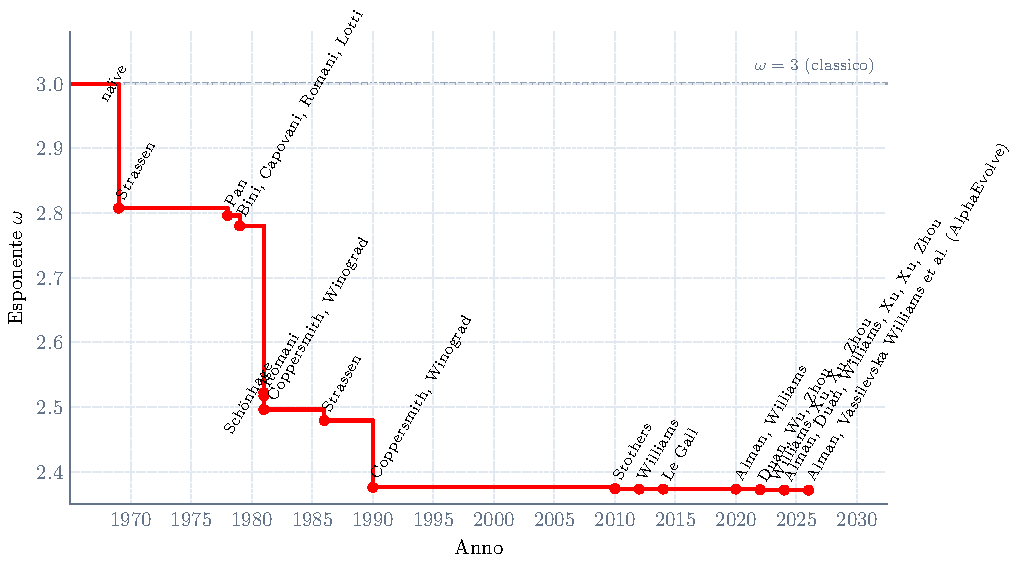
\includegraphics[width=0.9\textwidth, keepaspectratio]{Sources/Chapter3/figures/matrix_multiplication_timeline.pdf}
  \caption{Miglioramenti del limite superiore dell'esponente della moltiplicazione matriciale $\omega$ dal 1969 ad oggi. La linea tratteggiata rappresenta il limite superiore $\omega \le 3$.}
  \label{fig:matrix_mult_timeline}
\end{figure}

\begin{remark}
  Nella maggior parte della applicazioni, l'algoritmo di Strassen è quello ottimale, si
  veda la discussione in \cite{dalberto2023strassensmatrixmultiplicationalgorithm}. Di recente,
  il problema di stimare $ \omega $ e trovare il rango di tensori è diventato un problema
  d'interesse della branca della teoria della complessità algebrica e della geometria algebrica. Si
  veda ad esempio~\cite{landsberg2011tensors}.
\end{remark}


\section{Decomposizione low-rank di forme bilineari}

\todo{Spostare davanti alla CP per alleggerire (già scritta)}
Nel calcolo della complessità, le decomposizioni low-rank possono ridurre notevolmente le operazioni
aritmetiche sulle matrici. Se ad esempio $ M \in \R^{m\times n} $ è una matrice di rango uno, possiamo scrivere $ M =
u \topp v = uv^{\top} $ per certi $ u \in \R^m $ e $ v \in \R^n $; valutare $ Mx =
(uv^{\top})x = u(v^{\top}x) $ ha costo $ O(n) $, contro il costo $ O(mn) $ del prodotto classico
matrice vettore. In generale, se $ M $ ha rango $ R $, possiamo scriverla come somma di $ R $
matrici di rango uno\todo{aggiungere thm?} ed
ottenere un costo $ O(Rn) $ per $ Mx $. È possibile riadattare quest'idea per forme bilineari, come vedremo ora.

Calcolare la valutazione di una forma bilineare $ f $ come nell'Equazione~\ref{eq:b_k_bil} ha un costo $
  O(mnp) $, data dal numero di
  moltiplicazioni necessarie fra gli elementi di $ x $ e $ y $. Queste sono dette \emph{active
  multiplications} e corrispondono al numero di elementi non nulli di $ T $. Ci aspettiamo che
  la complessità di valutare $ f(x,y) $ sia correlata al costo delle active multiplications. Cerchiamo di minimizzarne il numero cercando fattorizzazioni CP di $ T $.


\begin{definition}[Bilinear algorithm]
  Sia $ \varphi : U \times V \to  W $ una mappa bilineare tra $ \K $-spazi vettoriali. Per ogni $ i
  \in \{1, \dots, r\} $, siano $ f_{i} \in U^*, g_{i} \in V^*, w_{i} \in W$ tali che
  \begin{equation*}
    \varphi(u,v) = \sum_{i=1}^r f_{i}(u)g_{i}(v)w_{i},
  \end{equation*}
  per ogni $ u \in U, v \in V$. Allora la $ r $-upla $ (f_1,g_1,w_1; \ldots ; f_r, g_r,w_r) $ viene
  detta \emph{bilinear computation (algorithm) di lunghezza $ r $ per $ \varphi $}, e la lunghezza
  di più breve algoritmo di calcolo per $ \varphi $ è chiamata \emph{bilinear complexity} o rango
  di $ \varphi $, che indichiamo ancora con $ \rk(\varphi) $.
\end{definition}


\begin{proposition}[Strassen]
  Siano $ U,V $ e $ W $ dei $ \K $-spazi vettoriali finiti, e $ \varphi : U\times V \to  W $ una
  mappa bilineare. Allora
  \begin{equation*}
    L(\varphi) = \text{Lunghezza della più breve bilinear computation per } \varphi.
  \end{equation*}
\end{proposition}
\begin{remark}
  Da questa proposizione segue direttamente che
  \begin{equation}
    \label{eq:LandRank_estimate}
    L(\varphi) \le \rk(\varphi) \le 2L(\varphi).
  \end{equation}
\end{remark}



La prossima definizione assicura che il rango di una forma bilineare è dato dal rango CP.
\begin{proposition}
  Fissata una forma bilineare $ \varphi $, e detto $ T $ il tensore che la rappresenta. Allora, dalla
  fattorizzazione CP di un tensore $ T $ si ottieme una bilinear computation, e in particolare $
  \rk(\varphi) = \rk(T) $.
\end{proposition}
\begin{proof}
Data una decomposizione $ T = \dsqr{U,V,W} $ di rango $ r $, dalla Definizione~\ref{def:CP}
abbiamo che $ T = \sum_{l=1}^r u_l \topp v_l \topp w_l $, o in componenti, $ T_{i,j,k} =
\sum_{l=1}^r u_{il}v_{jl}w_{kl} $. Inserendo questa relazione nell'Equazione~\ref{eq:b_k_bil} troviamo,

\begin{equation}
  \label{eq:b_active}
  \begin{aligned}
    \varphi_k(x,y) &= \left( \left( \sum_{l=1}^r u_l \topp v_l \topp w_l \right) \ttm[1] x^{\top} \ttm[2]
  y^{\top}  \right)_k  
             = \left( \sum_{l=1}^r \left( u_l \topp v_l \topp w_l  \right) \ttm[1] x^{\top} \ttm[2]
    y^{\top} \right)_k  \\ 
             &=
  \sum_{i=1}^m \sum_{j=1}^n \sum_{l=1}^r u_{il}v_{jl}w_{kl} x_i y_j = \sum_{l=1}^r \left(\sum_{i=1}^m 
    u_{il} x_i \right) \cdot \left( \sum_{j=1}^n v_{jl} y_j  \right)  w_{kl} \\
             &= \sum_{l=1}^r
   (u_l^{\top}x) \cdot (v_l^{\top}y)w_{kl},
  \end{aligned}
\end{equation}
per ogni $ k = 1, \ldots, p $.
Mettendo insieme le Equazioni \ref{eq:b_tuv} e \ref{eq:b_active} troviamo
\begin{equation}
  \label{eq:lowrank_bilinear}
  \varphi(x,y) = \sum_{l=1}^r (u_l^{\top}x)\cdot(v_l^{\top}y)w_l.
\end{equation}
Considerando i funzionali $ f_{l}(x) \defeq u_{l}^{\top}x $ e $ g_{l}(y) \defeq v_{l}^{\top}y $
indotti dal prodotto scalare standard si ha la tesi.

\end{proof}
Quindi valutare $ \varphi $ richiede esattamente $ r = \rk(T) $ active multiplications (e $
  O(r) $ addizioni), che sopra evidenziamo con $
(\cdot) $.
In particolare, il seguente risultato algebrico ci dice che la rappresentazione di una forma
bilineare come tensore o come bilinear computation sono identiche, ed è utile per riscrivere un
algoritmo tramite un tensore. 
\begin{proposition}[Si veda~\cite{burgisser2013algebraic}, Cap. 14]
  \label{prop:iso_bil_tensor}
  Siano $ U,V $ e $ W $ dei $ \K $-spazi vettoriali. Allora esiste un unico isomorfismo $ U^*
  \otimes V^* \otimes W \to \{\varphi : U \times V \to  W, \text{ bilineare}\} $ che manda $ f
  \otimes g \otimes w $ nella mappa bilineare $ (u,v) \mapsto f(u)g(u)w $.
\end{proposition}
\begin{definition}[Tensore strutturale]
  L'unico tensore $ T \in U^* \otimes V^* \otimes W$ associato alla mappa bilineare $ \varphi : U
  \times V \to W $ è detto \emph{tensore strutturale} di $ \varphi $.
\end{definition}


\section{Rappresentazione del prodotto tra matrici}

Consideriamo due matrici $ A \in \R^{M \times N} $ e $ B \in \R^{N \times P} $ e il loro prodotto $
C \in \R^{M \times P} $. Ponendo $ x =
\Vec(A) $ e $ y=\Vec(B) $, l'Equazione~\ref{eq:b_tuv} diventa 
\begin{equation}
  \label{eq:mulvec}
\Vec(C^\top) =\varphi(x,y) = T \ttm[1] \Vec(A)^{\top} \ttm[2] \Vec(B)^{\top}
,\end{equation}

dove abbiamo fissato l'ordinamento naturale sulle entrate di $ \Vec(A) $ e $ \Vec(B) $, e quello
inverso su $
\Vec(C^\top)$. Da ciò troviamo un tensore $ T \in \R^{MN\times NP\times MP} $ che rappresenta
la moltiplicazione tra $ \algob{M,N,P} $.
Data una decomposizione CP di rango $ r $ del tensore $ T  = \dsqr{U,V,W}$,
grazie all'Equazione~\ref{eq:lowrank_bilinear}, l'espressione sopra si traduce in
\begin{equation}
  \label{eq:mulvec:CP}
  \Vec(C^\top) =  \sum_{l=1}^r (u_l^\top \Vec(A)) \cdot
  (v_l^\top\Vec(B))w_l = \sum_{l=1}^r (s_l \cdot
  t_l)w_l = \sum_{l=1}^r m_lw_l,
\end{equation}
Dove abbiamo posto $ s_l \defeq  s_{l}(A) \defeq  u_l^\top \Vec(A)$, $ t_l \defeq t_{l}(B) \defeq v_l^\top\Vec(B)$ e $ m_l \defeq
s_lt_l $. Nella pratica, nei passaggi successivi dell'algoritmo calcoliamo in maniera ricorsiva il
prodotto tra $ s_l $ e $ t_l $.
Questa formula definisce un algoritmo di moltiplicazione veloce $ \algob{M,N,P} $.

\begin{figure}[htbp]
  \centering
  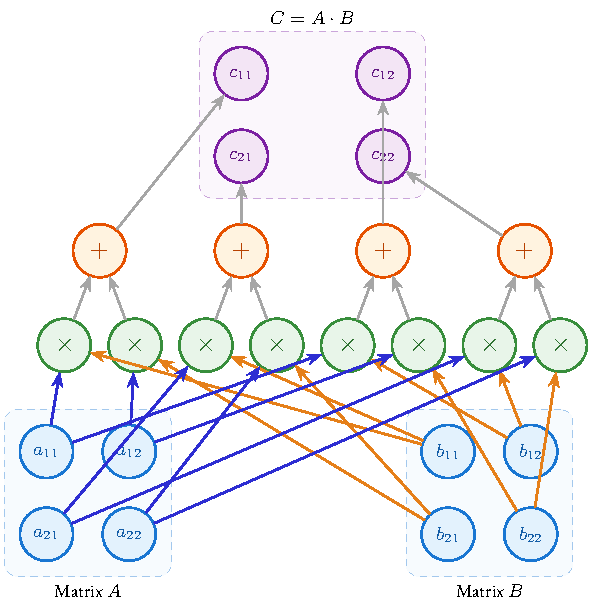
\includegraphics{Sources/Chapter3/figures/circuit.pdf}
  \caption{Circuito aritmetico per la moltiplicazione di matrici $2 \times 2$.}
  \label{fig:arithmetic_circuit_222}
\end{figure}


\section{Alcune stime sull'esponente}
\label{sec:exp_estimates}
Dal ragionamento sopra, $ \rk(\algob{n}) $ è dato dal numero di active multiplication nella molitiplicazione
di due matrici, e quindi ne misura la complessità algoritmica. Possiamo quindi riscrivere $ \omega $ come
\begin{equation}
  \label{eq:omega_as_rank}
  \omega = \lowlim_{n \to +\infty} \log_n \left( \rk(\algob{n}) \right).
\end{equation}
\todo{FIX errore nella formula}
Ad esempio, l'algoritmo di Strassen~\cite{strassen69} mostra che $ \rk(\algob{2}) \le 7$, e
come dimostrato da Winograd~\cite{winograd1971}, $ \rk(\algob{2}) = 7$, ovvero non è possibile moltiplicare due
matrici $ 2\times 2 $ con meno di sette moltiplicazioni.
Nei casi diversi da $ \algob{2} $ il problema si complica, e attualmente abbiamo alcune stime più lasche: già
per matrici $ 3\times 3 $, sappiamo solo che $ 19 \le \rk(\algob{3}) \le 23 $~\cite{BLASER200343,
bams/1183537626}, mentre la migliore stima astintotica dal basso per il caso di matrici $ n\times n $ è $ \frac{5}{2}n^2 - 3n \le
\rk(\algob{n}) $~\cite{blaser2001}. Si veda il capitolo 11 di~\cite{landsberg2011tensors} per
ulteriori dettagli e stime.


\subsection*{Trattare il caso generale}

Date due matrici $ n^i \times n^i $, possiamo vedere la loro moltiplicazione come la moltiplicazione
di matrici $ n\times n $ sull'algebra delle matrici $ n^{i-1}\times
n^{i-1} $, suddividendole in blocchi. Questo dice anche che, se $
\rk(\algob{n}) \le r $, allora $ \rk(\algob{n^i}) \le
  r^i$; infatti, combinando le prossime Proposizioni~\ref{prop:bil_map_product}
e~\ref{prop:rk_bil_map_product}, e usando che il rango è invariante per isomorfismo, troviamo
\begin{equation*}
  \rk(\algob{n^i}) = \rk(\algob{n}^{\otimes i}) \le \rk(\algob{n})^i \le r^i.
\end{equation*}
Quindi, possiamo applicare ricorsivamente l'algoritmo di moltiplicazione veloce, che è disegnato per
matrici $ n\times n $, per ottenere la moltiplicazione di matrici $ n^i \times n^i $ impiegando solo $ r^i $ moltiplicazioni.

Se invece $ n > n_0 $ sono due interi positivi, dato un algoritmo con un caso base fissato $
\algob{n_0} $, è possibile ottenerne uno per
$ \algob{n} $, con $ n >  n_0 $, allargando la matrice aggiungendo zeri
fino alla dimensione
$ n_0^{\left\lceil \log_{n_0} n \right\rceil } $. La complessità dipenderà comunque da $ n_0 $ e
da $ r $, in quanto
\begin{equation*}
  \begin{aligned}
    \rk(\algob{n}) &\le \rk(\algob{n_0^{\left\lceil \log_{n_0} n \right\rceil }}) && \text{dalla
    \ref{prop:rk_monotony},} \\
                  &\le \rk(\algob{n_0})^{\left\lceil \log_{n_0} n \right\rceil } && \text{dalle
    \ref{prop:bil_map_product} e \ref{prop:rk_bil_map_product},}\\
                  &\le r^{\left\lceil \log_{n_0} n \right\rceil } && \text{per ipotesi $
  \rk(\algob{n}\le r $,} \\
                  &\le r \cdot n^{\log_{n_0} r} && \text{usando che $ \left\lceil x \right\rceil \le
                  x+1$}.
  \end{aligned}
\end{equation*}
Riassumendo, $ \rk(\algob{n,n,n}) \le r \cdot n^{\log_{n_0} r} $. Dunque ignorando la costante e
dall'Equazione~\ref{eq:omega_as_rank}, $ \omega \le \log_{n_0} r $. Ad esempio, per
l'algoritmo di Strassen poniamo $ r = 7,n_0 = 2 $, da cui $ \omega \le \log_{2} 7 < 2.81 $. Abbiamo
dimostrato la seguente:
\begin{proposition}
  Se $ \rk(\algob{n}) \le r$ per degli interi positivi $ n,r $, allora $ n^\omega \le r $.
\end{proposition}

Nei passaggi sopra abbiamo anche osservato che se $ n \le n' $ e dato un algoritmo per $ n' $, possiamo ottenerne uno per $ n $
allargando la matrice. Possiamo racchiudere questa proprietà nel seguente risultato:
\begin{proposition}[Monotonia del rango di un algoritmo]
  \label{prop:rk_monotony}
Il rango di un algoritmo è monotono crescente rispetto alla dimensione, ovvero dati due interi positivi $ n \le n' $, allora $
\rk(\algob{n}) \le \rk(\algob{n'}) $.
\end{proposition}



Riportiamo le proposizioni utilizzate per dimostrare la proposizione sopra, dimostrate
in~\cite{burgisser2013algebraic}, Cap. 14,15.
\begin{proposition}
  \label{prop:bil_map_product}
  Siano $ e,e', h,h',l,l' $ degli interi positivi. Allora abbiamo
  \begin{equation*}
    \algob{e,h,l} \otimes \algob{e', h', l'}\simeq \algob{ee', hh', ll'},
  \end{equation*}
  cioè le due forme bilineari sono isomorfe.
\end{proposition}
\begin{proposition}
  \label{prop:rk_bil_map_product}
  Siamo $ \varphi_1,\varphi_2 $ due mappe bilineari. Allora $ \rk(\varphi_1 \otimes \varphi_{2}) \le
  \rk(\varphi_1)\rk(\varphi_2)$.
\end{proposition}

\section{Il rango come misura della complessità}

% La condizione trovata nell'Equazione~\ref{eq:omega_as_rank} è anche necessaria \todo{check}. 
La prossima proposizione mostra che il rango di un tensore è una misura ottimale della complessità.
Inoltre risponde all'esistenza del problema inverso: dato un intero positivo $ r $, è possibile
trovare un algoritmo con $ r $ moltiplicazioni? La risposta precisa è data dal seguente risultato.
\begin{theorem}[Strassen~\cite{strassen69}, vedi anche \cite{burgisser2013algebraic} §15.1]
  \label{thm:strassen}
  \begin{equation*}
    \omega = \inf \{\tau \in \R \mid \rk(\algob{n}) = O(n^\tau)\}.
  \end{equation*}
  Ovvero, è possibile moltiplicare due matrici $ n\times n $ usando $ O(n^{\omega + \varepsilon}) $
  operazioni aritmetiche se e solo se il rango tensoriale di $ \algob{n} $ è $
  O(n^{\omega+\varepsilon}) $.
\end{theorem}

Introduciamo alcuni strumenti utili a dimostrare questo risultato.
\begin{definition}[Mappa bilineare concise]
  Sia $ \varphi : U\times V \to  W$ una mappa bilineare. Diremo che $ \varphi $ è \emph{concise} se
  valgono tutte e tre le condizioni sotto:
  \todo{change to roman and to $ i $-concise per matchare quella dei tensori}
  \begin{enumerate}
    \item $\lKer(\varphi) = \{u \in U \mid \varphi(u,\cdot ) = 0\}  = \{0\} $,
    \item $\rKer(\varphi) = \{v \in V \mid \varphi(\cdot,v ) = 0\}  = \{0\} $,
    \item $\Im(\varphi) = \{\varphi(u,v) \mid u\in U, v\in V\} = W$.
  \end{enumerate}
\end{definition}
\begin{remark}
  \todo{osservare che combacia con la def data per i tensori}
\end{remark}
\begin{example}
  La mappa bilineare $ \algob{n} $ è concise.
\end{example}

\begin{lemma}
  \label{lemma:rec_relation_ab}
  Sia $ x = \left( x_0, x_1, x_2,\ldots \right) $ una successione di numeri reali che soddisfa la
  ricorsione $ x_s = ax_{s-1} + cb^s $, per certi numeri reali $ a,b,c $. Allora per ogni $ s \ge 0
  $, vale
  \begin{equation*}
    x_s = \begin{cases}
      a^s x_0 + (a^s - b^s) \frac{bc}{a-b} & \text{se } a\neq b, \\
      (cs + x_0)a^s & \text{se } a = b.
    \end{cases}
  \end{equation*}
\end{lemma}
\begin{proof}
  Mostriamo la formula per induzione su $ s $. Per $ s=0 $ la formula è verificata.
  \begin{equation*}
    \begin{aligned}
    x_1 &= ax_0 + bc, \\
    x_2 &= a(ax_0 + bc) + b^2 c \\
        &= a^2 x_0 + (a + b)bc \\
        &= \begin{cases}
          a^2x_0 + (a^2 - b^2)\frac{bc}{a-b} & \text{se } a\neq b, \\
          (2c + x_0)a^2 & \text{se } a=b.
        \end{cases}
    \end{aligned}
  \end{equation*}
  Assumiamo la proprietà vera per $ n-1 $ e mostriamola per $ n $.

  Se $ a \neq b $, 
  \begin{equation*}
    \begin{aligned}
      x_s &= a\left(a^{s-1}x_0 + \left(a^{s-1} - b^{s-1}\right) \frac{bc}{a-b}\right) + b^sc \\
          &= a^s x_0 + \left( (a^{s-1} - b^{s-1})a + b^{s-1}(a-b) \right)\frac{bc}{a-b} \\
          &= a^s x_0 + \left(a^{s}-b^{s} \right)\frac{bc}{a-b}
    \end{aligned}
  \end{equation*}

  Similmente, se $ a = b $
  \begin{equation*}
    \begin{aligned}
      x_s &= \left( c(s-1) + x_0 + c \right)a^s \\
          &=  (cs + x_0)a^s.
    \end{aligned}
  \end{equation*}
\end{proof}

\begin{proof}[Dimostrazione del Teorema di Strassen]
  Dimostriamo che 
  \begin{equation*}
    \omega = \inf \{\tau \in \R \mid \rk(\algob{n}) = O(n^\tau)\}.
  \end{equation*}
  Sia $ \theta $ il lato destro dell'equazione sopra, e per semplicità scriviamo $ M(n) \defeq
  M_{\K}(n)$ e $ \omega \defeq \omega_{\K}$. Dall'Equazione~\ref{eq:LandRank_estimate} abbiamo
  \begin{equation*}
    \frac{1}{2}R(\algob{n}) \le L(\algob{n}) \le M(n),
  \end{equation*}
  e dalla Definizione~\ref{def:exponent_matmul} segue $ \theta \le \omega $.

  Mostriamo che $ \omega \le \theta $. Per definizione di $ \theta $, per ogni $ \varepsilon >0 $
  esiste un $ n>1 $ tale che
  \begin{equation}
    \label{eq:r_estimate}
    r \defeq \rk(\algob{n}) \le n^{\theta + \varepsilon}.
  \end{equation}
  
  Dall'Equazione~\ref{eq:mulvec:CP}\todo{matrix product, ma TODO verifica, e controlla se è così davvero( io ho i vec)} esistono dei funzionali $ f_{\rho},g_{\rho} \in
  (\K^{n\times n})^*$  e delle matrici $ w_{\rho} \in \K^{n\times n} $ per $ \rho \in \{1, \ldots,
  r\}  $ tali che, per ogni $ A,B \in \K^{n\times n} $
  \begin{equation*}
    AB = \sum_{\rho = 1}^r f_{\rho}(A)g_{\rho}(B) w_{\rho}.
  \end{equation*}
  Vedendo $ \mathcal{A} = \K^{n^i\times n^i} $ come l'algebra delle matrici $ n^i \times n^i $, notiamo che i funzionali $ f_{\rho}, g_{\rho} : \K^{n\times n} \to \K $ si estendono a funzionali
  $ f_{\rho}, g_{\rho} : \mathcal{A}^{n\times n} \to \mathcal{A} $, sostituendo le entrate scalari
  con delle matrici. In particolare vale, per ogni $ A,B \in \mathcal{A}^{n\times n} $
  \begin{equation}
    \label{eq:blk_matmul_algo}
    AB = \sum_{\rho = 1}^r f_{\rho}(A)g_{\rho}(B) w_{\rho}.
  \end{equation}
L'Equazione sopra rappresenta l'algoritmo di moltiplicazione a blocchi tra $ A
  $ e $ B $: infatti abbiamo $ \mathcal{A}^{n\times n} = (\K^{n^i\times n^i})^{n \times n} \simeq \K^{n^{i+1}
  \times n^{i+1}} $, dove l'isomorfismo è dato dalla decomposizione in blocchi. Da questo fatto,
  unito all'Equazione~\ref{eq:blk_matmul_algo}, si
  ottiene che
  \begin{equation}
    \label{eq:Mn_recursionleq}
    M(n^{i+1}) \le r M(n^i) + cn^{2i},
  \end{equation}
  dove $ c \defeq c(n,r) $ è una costante che dipende sia da $ n $ che da $ r $. Questo perché nella
  formula il prodotto $ AB $, sviluppato come prodotto tra blocchi $ n^i \times n^i $ (formalmente, visto come prododotto a coefficienti in $ \mathcal{A} $), coinvolge $ r $ prodotti e
  un numero costante di addizioni.
  Siccome $ \algob{n} $ è concise, abbiamo che $ r \ge n^2 $. Fissando $ n $ (e quindi $ r $),
  risolviamo la ricorsione dell'Equazione~\ref{eq:Mn_recursionleq} in funzione di $ i $ usando il
  Lemma~\ref{lemma:rec_relation_ab} con $ a = r $ e $ b = n^2 $, analizzando due casi.

  Se $ r > n^2 $, abbiamo che
  \begin{equation*}
    \begin{aligned}
      M(n^i) &= r^i M(1) + (r^i - n^{2i})\frac{n^2c}{r-n^2} \\
             &= (M(1) + n^2c)r^i - n^{2i}\frac{n^2c}{r-n^2},
    \end{aligned}
  \end{equation*}
  da cui, 
  \begin{equation*}
    M(n^i) \le \alpha r^i + \beta n^{2i},
  \end{equation*}
  dove abbiamo posto $ \alpha \defeq M(1) + n^2c $ e $ \beta \defeq - \frac{n^2c}{r-n^2}$. 

  Se $ r = n^2 $, dal Lemma~\ref{eq:Mn_recursionleq} abbiamo
  \begin{equation*}
    M(n^i) \le (cs + M(1))r^i,
  \end{equation*}

  In entrambi i casi troviamo,
  \begin{equation}
    \label{eq:Mn_as_O_ri}
    M(n^i) = O(r^i).
  \end{equation}
  Dalla proposizione~\ref{prop:rk_monotony} segue che $M$ è una successione monotona, da cui per ogni $ h = n^i \in \N \setminus \{0\}  $, 
  \begin{equation*}
    M(h) = O(r^{\log_{n}h}) = O(h^{\log_{n}r}) = O(h^{\theta + \varepsilon}),
  \end{equation*}
  dove la prima uguaglianza segue sostituendo, $ i = \log_n h$
  nell'Equazione~\ref{eq:Mn_recursionleq}, la seconda da una proprietà del logaritmo, e la terza
  applicando la stima dell'Equazione~\ref{eq:r_estimate}.
  Quindi $ \omega_{\K} \le \theta $, che completa la dimostrazione.
\end{proof}

\section{Algoritmi di moltiplicazione veloce}

\begin{remark}
  \label{rem:rectangular}
  Di seguito ci limiteremo a studiare prodotti fra matrici quadrate; per il caso rettangolare, si
  possono estendere i ragionamenti sopra considerando una rappresentazione di rango $ r $ del
  tensore $ \algob{m,n,p} $ e scrivendo, attraverso una serie di permutazioni cicliche, la fattorizzazione di $ \algob{mnp} $ di rango $ r^3 $, che produce un algoritmo di complessità $ O(n^{\log_{abc}r^3}) =
  O(n^{3\log_{abc}r})$. Questo si può vedere tramite la scrittura della moltiplicazione tra matrici
  come forma trilineare dell'Osservazione~\ref{rmk:triliear_matmul} ci assicura che il tensore è
  invariante per trasformazioni cicliche, in quanto
  \begin{equation}
    \mathop{trace}(ABC) = \mathop{trace}(CAB) = \mathop{trace}(BAC).
  \end{equation}
\end{remark}


\subsection*{Il caso naive}
\todo{Dire se la derivazione del tensore è chiara, ho provato a giustificarla meglio che potessi}

Trattiamo il caso di matrici quadrate con taglie potenze di due (possiamo farlo a meno di passare a
una sottomatrice di taglia pari). In questo caso possiamo
partizionare le matrici in delle sottomatrici a blocchi $ 2\times 2 $ \footnote{possiamo pensare alle entrate
sia come scalari, che come matrici.}:
\begin{equation*}
  \begin{bmatrix}
    c_{11} & c_{12} \\
    c_{21} & c_{22}
  \end{bmatrix} =
  \begin{bmatrix}
    a_{11} & a_{12} \\
    a_{21} & a_{22}
  \end{bmatrix} \cdot 
  \begin{bmatrix}
    b_{11} & b_{12} \\
    b_{21} & b_{22}
  \end{bmatrix} =
  \begin{bmatrix}
    a_{11}b_{11} + a_{12}b_{21} & a_{11}b_{12} + a_{12}b_{22} \\
    a_{21}b_{11} + a_{22}b_{21} & a_{21}b_{12} + a_{22}b_{22}
  \end{bmatrix}.
\end{equation*}
L'algoritmo naive procede combinando un insieme di otto moltiplicazioni matriciali con quattro
addizioni:

\begin{equation}
\label{eq:mult_222_m_i}  
\begin{aligned}
m_1 &= a_{11} \cdot b_{11} = s_1 t_1&\quad m_2 &= a_{12} \cdot b_{21} = s_2t_2 &\quad m_3 &= a_{11}
\cdot b_{12} = s_3t_3 \\
m_4 &= a_{12} \cdot b_{22} = s_4t_4 &\quad m_5 &= a_{21} \cdot b_{11} = s_5t_5 &\quad m_6 &= a_{22}
\cdot b_{21} = s_6t_6 \\
m_7 &= a_{21} \cdot b_{12} = s_7t_7 &\quad m_8 &= a_{22} \cdot b_{22} = s_8t_8 & &
\end{aligned}
\end{equation}

\[
\begin{aligned}
 c_{11} &= m_1 + m_2 = a_{11}b_{11} + a_{12}b_{21}, &\qquad  c_{12} &= m_3 + m_4 = a_{11}b_{12} +
a_{12}b_{22}, \\
 c_{21} &= m_5 + m_6 = a_{21}b_{11} + a_{22}b_{21}, &\qquad  c_{22} &= m_7 + m_8 = a_{21}b_{12} +
a_{22}b_{22}.
\end{aligned}
\]

\begin{figure}[htbp]
  \centering
  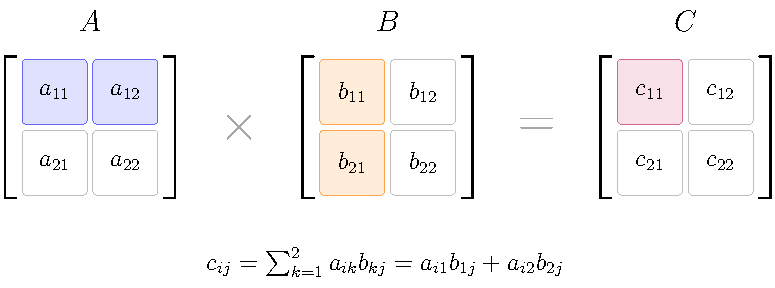
\includegraphics{Sources/Chapter3/figures/matrix_multiplication_linear.pdf}
  \caption{Rappresentazione della moltiplicazione di due matrici $2 \times 2$.}
  \label{fig:matrix_multiplication_linear}
\end{figure}

Proviamo a scriverlo in forma tensoriale. La sua bilinear computation è
\begin{equation*}
  C = \sum_{i=1}^8 m_{i}w_{i}
\end{equation*}
Usando l'Osservazione~\ref{rmk:triliear_matmul} possiamo scrivere $ \algob{2} $ come mappa
trilineare come
\begin{equation*}
  \begin{aligned}
    \mathop{trace}(ABC) &= 
    \mathop{trace}\left(
    \begin{bmatrix} 
    s_1t_1 + s_2t_2 & s_3t_3 + s_4t_4 \\
    s_5t_5 + s_6t_6 & s_7t_7 + s_8t_8
    \end{bmatrix} 
    \begin{bmatrix} c_{11} & c_{12} \\ c_{21} & c_{22} \end{bmatrix} 
    \right) \\
                           &= (s_1t_1 + s_2t_2)c_{11} + (s_3t_3 + s_4t_4)c_{21}+ (s_5t_5 +
                           s_6t_6)c_{12} + (s_7t_7 + s_8t_8)c_{22}.
  \end{aligned}
\end{equation*}
Tramite l'isomorfismo della Proposizione~\ref{prop:iso_bil_tensor}, possiamo mappare ogni termine $
s_{r}t_{r}w_{r}$ dell'equazione sopra in $ s_{r} \otimes t_{r} \otimes c_{r}$ e scrivere il tensore struttrale di $
\algob{2} $ in formato CP:
e visualizzarlo nella Figura~\ref{fig:tensor_222_cp}:
\begin{equation}
  \label{eq:tensor_222}
  \begin{aligned}
    \algob{2} &= a_{11} \topp b_{11}\topp c_{11} + a_{12}\topp b_{21} \topp c_{11} \\
                 &+ a_{21}\topp b_{11} \topp c_{21} + a_{22} \topp b_{21} \topp c_{21} \\ 
                 &+ a_{11} \topp b_{12} \topp c_{12} + a_{12} \topp b_{22} \topp c_{12} \\
    &+ a_{21} \topp b_{12} \topp c_{22} + a_{22}\topp b_{22}\topp c_{22}.
  \end{aligned}
\end{equation}


\begin{figure}[htbp]
  \centering
  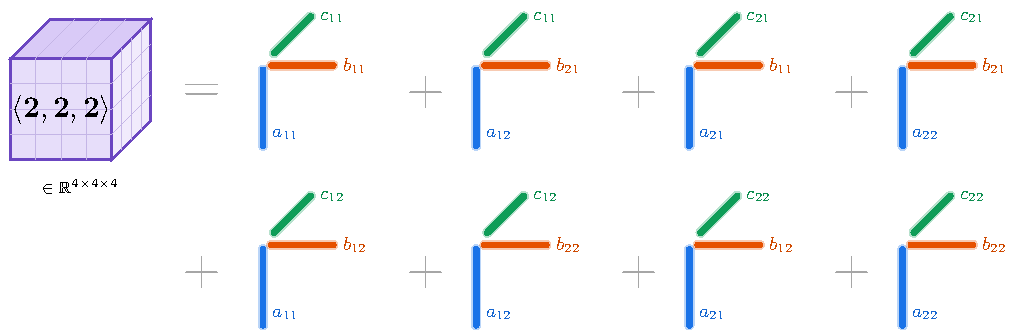
\includegraphics[width=\textwidth]{Sources/Chapter3/figures/tensor_222_cp.pdf}
  \caption{Decomposizione CP del tensore di moltiplicazione di matrici $ \algob{2} $ come somma di 8 tensori di rango uno.}
  \label{fig:tensor_222_cp}
\end{figure}



Per secoli questo algoritmo è stato ritenuto il più veloce per moltiplicare le matrici. Nel ??
Strassen \footnote{in una comunicazione riportata da Landsberg in~\cite{landsberg2011tensors}.}
tentò di mostrare che non esistesse un algoritmo più veloce, fallendo in maniera spettacolare \footnote{in realtà
la tesi è vera nel campo $ \Z/2\Z $.} e dando vita a una nuova teoria.

\subsection*{L'algoritmo di Strassen}

L'algoritmo di Strassen è probabilmente l'algoritmo di moltiplicazione veloce più noto e segue la
stessa struttura a blocchi $ \algob{2} $.

\begin{align*}
s_1 &= a_{11} + a_{22} & s_2 &= a_{21} + a_{22} & s_3 &= a_{11} \\
s_4 &= a_{22} & s_5 &= a_{11} + a_{12} & s_6 &= a_{21} - a_{11} \\
s_7 &= a_{12} - a_{22} \\
t_1 &= b_{11} + b_{22} & t_2 &= b_{11} & t_3 &= b_{12} - b_{22} \\
t_4 &= b_{21} - b_{11} & t_5 &= b_{22} &t_6 &= b_{11} + b_{12} \\
t_7 &= b_{21} + b_{22}
\end{align*}
\begin{align*}
m_r &= s_rt_r, \quad 1 \le r \le 7 \\
c_{11} &= m_1 + m_4 - m_5 + m_7 & c_{12} &= m_3 + m_5 \\
c_{21} &= m_2 + m_4 & c_{22} &= m_1 - m_2 + m_3 + m_6
\end{align*}

\todo{Aggiungere tensore}
\todo{aggiungere costo}

\section{Algoritmi APA}
\label{sec:APA}

Dopo il tentativo di Strassen di dimostrare che l'algoritmo di moltiplicazione standard fosse
ottimale, Bini et. Al~\cite{bini1980relations} considerano il seguente algoritmo di moltiplicazione ridotto ottenuto
ponendo a zero l'entrata $ a_{22} $ di $ \algob{2} $:
\begin{equation*}
  \begin{bmatrix}
    a_{11} & a_{12} \\
    a_{21} & 0
  \end{bmatrix} \cdot 
  \begin{bmatrix}
    b_{11} & b_{12} \\
    b_{21} & b_{22}
  \end{bmatrix} =
  \begin{bmatrix}
    a_{11}b_{11} + a_{12}b_{21} & a_{11}b_{12} + a_{12}b_{22} \\
    a_{21}b_{11}  & a_{21}b_{12} 
  \end{bmatrix}.
\end{equation*}
Facendo alcuni raccoglimenti e sostituendo $ a_{22} =0$, il tensore dell'Equazione~\ref{eq:tensor_222} si riscrive come
\begin{equation*}
  \begin{aligned}
    \algob{2}^{\text{red}}
    &\defeq a_{11} \topp (b_{11} \topp c_{11} + b_{12} \topp c_{12})
                              + a_{12} \topp (b_{21} \topp c_{11} + b_{22} \topp c_{12})\\ 
                              &+ a_{21} \topp (b_{11} \topp c_{21} + b_{12}
  \topp c_{22}).
  \end{aligned}
\end{equation*}

Che è somma di sei tensori elementari distinti, quindi $ \rk{\algob{2}^{\text{red}}} \le 6 $.
Bini et. al. provarono a cercare un'espressione di rango cinque per $ \algob{2}^{\text{red}} $
numericamente, calcolando
\begin{equation*}
  \min_{\substack{T \in \R^{n\times n\times n} \\ \rk(T) = 5}}{\| \algob{2}^{\text{red}} - T\| }
\end{equation*}
 norma di $ \algob{2}^{\text{red}} $. Il loro computer continuava a produrre tensori $ T $ di rango cinque
con la norma della differenza che diventava sempre più piccola, ma con coefficienti sempre più
grandi. Questo è andato avanti per un po' di tempo, fino a che realizzarono che il codice era
giusto, ma quello che sembrava un problema era in realtà una manifestazione di un fenomeno chiamato \emph{border rank}.
L'espressione del tensore che stavano cercando era il seguente tensore di rango $ 5 $:
\begin{equation*}
  \begin{aligned}
    \algob{n}_t^{\text{red}} = \frac{1}{t} \left[ (I) + (II) -(III) - (IV) + (V)
    \right],
  \end{aligned}
\end{equation*}
dove 
\begin{equation*}
  \begin{aligned}
    (I) &= (x_2^1 + tx_1^1) \otimes (y_2^1 + ty_2^2 \otimes z_2^1) \\
        &= x_{2}^1 \otimes y_2^1 \otimes z_2^1 + t[x_2^1 \otimes y_2^2 \otimes z_2^1 + x_1^1 \otimes
        y_2^1 \otimes z_2^1] + O(t^2) \\
    (II) &= (x_1^2 + tx_1^1) \otimes y_1^1 \otimes (z_1^1 + tz_1^2) \\
         &= x_1^2 \otimes y_1^1 \otimes z_1^1 +t[x_1^2 \otimes y_1^1 \otimes z_1^2 + x_1^1 \otimes
         y_1^1 \otimes z_1^1] + O(t^2) \\
    (III) &= x_1^2 \otimes y_1^1 \otimes z_1^1 + t[x_1^2 \otimes y_1^1 \otimes z_1^2 + x_1^1 \otimes
    y_1^1 \otimes z_1^1] + O(t^2) \\
    (IV) &= x_1^2 \otimes ((y_1^1 + y_2^1) + ty_1^2) \otimes z_1^1 \\
         &= x_1^2 \otimes y_1^1 \otimes z_1^1 + x_1^2 \otimes y_2^1 \otimes z_1^1 + t[x_1^2 \otimes
         y_1^2 \otimes z_1^1] \\
    (V) &= (x_2^1 + x_1^2) \otimes (y_2^1 + ty_1^2) \otimes (z_1^1 + tz_2^2) \\
        &=x_2^1\otimes y_2^1 \otimes z_1^1 + x_1^2 \otimes y_2^1 \otimes z_1^1 \\
        &+ t[x_2^1 \otimes
        (y_2^1 + z_2^2 + y_1^2 \otimes z_1^1) + x_1^2 \otimes (y_2^1 \otimes z_2^2 + y_1^2 \otimes
        z_1^1)] + O(t^2)
  \end{aligned}
\end{equation*}
In ogni passaggio abbiamo applicato più volte la proprietà distributiva del prodotto tensoriale.
Osserviamo che i termini di grado costante in $ t $ si cancellano:
\begin{equation*}
  \begin{aligned}
    x_2^1 &\otimes (y_2^1 \otimes z_2^1 - y_2^1 \otimes z_1^1 - y_2^1 \otimes z_2^1 + y_2^1 \otimes
    z_1^1) \\
    + x_1^2 &\otimes (y_1^1 \otimes z_1^1 - y_1^1 \otimes z_1^1 + y_2^1 \otimes z_1^1 - y_2^1 \otimes z_1^1)
    = 0
  \end{aligned}
\end{equation*}
Sommando e raggruppando i termini di grado uno in $ t $ troviamo
\begin{equation*}
  \begin{aligned}
   \algob{n}^\text{red} = x_1^1 &\otimes (y_1^1 \otimes z_1^1 + y_2^1 \otimes z_2^1) +\\
    x_2^1 &\otimes (y_1^2 \otimes z_1^1 + y_2^2 \otimes z_2^1) + \\
    x_1^2 &\otimes (y_1^1 \otimes z_1^2 + y_2^1 \otimes z_2^2),
  \end{aligned}
\end{equation*}
ovvero il tensore di partenza. Da cui,
\begin{equation*}
  \algob{n}_t^{\text{red}} - \algob{n}^{\text{red}} = O(t^2) \to 0
\end{equation*}
Abbiamo dimostrato che un tensore di rango $ 5 $ converge a uno di rango $ 6 $.

\subsection*{Il problema del border rank}
\label{sec:border_rank}

\todo{Introduci e motiva il problema partendo dagli algoritmi APA (vedi Landsbeg)}

\begin{example}
  \label{ex:border_rank}
  Consideriamo dei vettori $ a_1,a_2 \in \R^m$, $b_1,b_2 \in \R^n$ e $c_1,c_2\in \R^p $ vettori
  linearmente indipendenti. Definiamo il tensore 
  \begin{equation}
    T = a_1 \topp  b_1 \topp c_2 + a_1 \topp b_2 \topp c_1 + a_2 \topp b_1 \topp c_1,
  \end{equation}
  e notiamo che $ \rk(T) = 3 $ dato che non può
  essere scomposto come somma di tensori più semplici.
  Consideriamo la successioni di tensori 
  \begin{equation}
  \label{eq:rank_counterex}
  T_\varepsilon = \frac{1}{\varepsilon}\left( a_1 +
  \varepsilon a_2 \right) \topp (b_1 + \varepsilon b_2) \topp (c_1 + \varepsilon c_2) -
  \frac{1}{\varepsilon} a_1 \topp b_1 \topp c_1, \text{ con } \varepsilon \in \R,
  \end{equation}
  che essendo combinazione lineare di due tensori di rango uno, ha rango 2.
  Vediamo che $ \lim_{\varepsilon \to 0} T_\varepsilon = T $, da cui segue che l'insieme dei tensori di rango 3 non è chiuso.
  Espandendo i termini dell'Equazione \ref{eq:rank_counterex} tramite la proprietà distributiva del prodotto esterno,
  \begin{equation}
    \begin{aligned}
      \Tn{y}_\varepsilon &=  \frac{1}{\varepsilon} a_1 \topp b_1 \topp c_2 + a_1 \topp b_1 \topp c_2 + a_1 \topp b_2 \topp c_1
      +a_2 \topp b_1 \topp c_1  \\ &+ \varepsilon \left(a_2 \topp b_2 \topp c_1 + a_1 \topp b_1 \topp c_2 +
      a_1 \topp b_2 \topp c_2 + a_2 \topp b_2 \topp c_2 \right) - \frac{1}{\varepsilon} a_1 \topp
      b_1 \topp c_1 \\
                         &= T + \varepsilon\left(a_2 \topp b_2 \topp c_1 + a_1 \topp b_1 \topp c_2 +
      a_1 \topp b_2 \topp c_2 + a_2 \topp b_2 \topp c_2 \right)
    \end{aligned}
  \end{equation}
  Quindi $ T_\varepsilon - T \to 0 $.
\end{example}

Questo motiva la seguente definizione:


\begin{definition}[Border rank]
  Un tensore $ T $ ha \emph{border rank} $ r $ se è limite di una successione di tensori di
  rango $ r $, ma non è limite di una successione di tesori di rango $ s $, per ogni $ s < r $. Lo
  denoteremo con il simbolo $ \brk(T) $.
\end{definition}
\begin{remark}
  $ \rk(T) \ge \brk(T) $.
\end{remark}
\begin{remark}
  In coordinate, se $ T \in \Rmsiz $, il suo border rank è la quantità
  \[
  \brk(T) = \min \left\{ r \in \N \mid \exists T' \in \Rmsiz! \text{ tale che }
  \rk(T')=r, \, \|T - T'\|  < \varepsilon \right\}
  .\] 
\end{remark}
\todo{Disegno interpretazione geometrica (landsberg pg 38)}

Il border rank si rivela utilissimo nello studio dell'esponente $ \omega $, cioè possiamo sostituire
il rango con il border rank nel Teorema~\ref{thm:strassen}:
\begin{theorem}[Bini~\cite{bini1980relations}, vedi \S3.2]
  \begin{equation*}
    \omega = \inf \{\tau \in \R \mid \brk(\algob{n}) = O(n^\tau)\} .
  \end{equation*}
\end{theorem}
Anche se potremmo avere $ \brk(\algob{n}) < \rk(\algob{n}) $, non sono abbastanza diversi da
avere un impatto sull'esponente\todo{why?}.

Riportiamo alcune stime sul border rank riportate in~\cite{landsberg2015geometry}, \S1. Per $ n = 2 $,
Winograd dimostra\todo{ref} che $ \brk(\algob{2}) = \rk(\algob{2}) = 7 $. Ci aspetteremmo che per $
n > 2 $, $ \brk(\algob{n}) < \rk(\algob{n}) $. Per $ n=3 $, sappiamo solo che $ 15 \le
\brk(\algob{3}) \le 20 $ e $ 19 \le \rk(\algob{3}) \le 23 $. In generale, sappiamo che $
\rk(\algob{n}) \ge  3n^2 - o(n) $ e $ \brk(\algob{n}) \ge 2n^2 - \left\lceil \log_{2}(n)
\right\rceil -1 $.

\section{Errore algoritmico}

\todo{discussione della stabilità dal paper dato dal prof}

% !TEX root = ../../Thesis.tex
%%%%%%%%%%%%%%%%%%%%%%%%%%%%%%%%%%%%%%%%%%%%%%%%%%%%%%%%%%%%%%%%%%%%%%%%
\chapter{Applicazioni modellistiche della decomposizione CP}
\label{chp:cp_applications}
%%%%%%%%%%%%%%%%%%%%%%%%%%%%%%%%%%%%%%%%%%%%%%%%%%%%%%%%%%%%%%%%%%%%%%%%
\todo{migliorato}
In questo capitolo esploreremo due applicazioni della decomposizione CP di un tensore a tre indici
in due ambiti modellistici,
dove avremo modo di applicare il Teorema di Kruskal~\ref{thm:kruskal3d} e l'algoritmo Alternating
Least Squares. Nel primo esperimento il rango non sarà noto a priori e dovremo prima approssimarlo,
per poi trovare una decomposizione. Nel secondo conosceremo il rango a priori.
In entrambi gli esperimenti sarà necessario risolvere l'ambiguità del riscalamento e della
permutazione dei fattori per preservare il modello reale.

\section{Spettroscopia fluorescente}

Nella \emph{spettroscopia fluorescente}, un campione chimico è eccitato e
la luce emessa viene misurata a diverse lunghezze d'onda, risultando in una matrice di
\emph{eccitazione-emissione} (EEM) di intensità fluorescenti (si veda Figura~\ref{fig:spectroscopy}). Quando i dati EEM vengono raccolti da
diversi campioni, otteniamo un tensore a tre indici. Questi dati si possono utilizzare nella chimica
analitica per stimare le concentrazioni e gli spettri dei composti chimici a
partire da più miscele.

\begin{figure}[htbp]
	\centering
	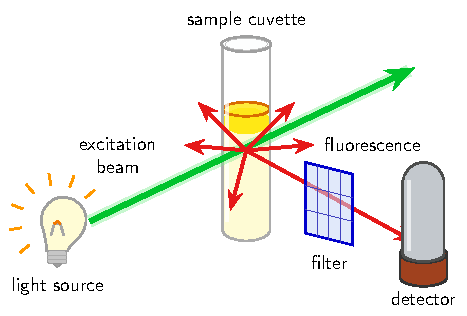
\includegraphics{Sources/Chapter4/figures/spectroscopy.pdf}
	\caption{Rappresentazione schematica di uno spettrofotometro per spettroscopia di fluorescenza.}
	\label{fig:spectroscopy}
\end{figure}

Nel dettaglio, vengono dati $ I $ campioni di soluzioni chimiche, ognuno dei quali contiene diverse sostanze
diluite in diverse concentrazioni. Il primo obiettivo è determinare il numero $ r $ delle diverse
sostanze presenti.
Il dataset che analizziamo~\cite{kolda2021eem,acar2014structure} è composto da una serie di esperimenti riportati
da~\cite{smilde2004multi}, nel quale sono presenti tre sostanze chimiche disciolte nelle soluzioni:
\begin{itemize}
	\item \emph{Valine-Tyrosine-Valine} (Val-Tyr-Val) - peptide,
	\item \emph{Tryptophan-Glycine} (Trp-Gly) - peptide,
	\item \emph{Phenylalanine} (Phe) - aminoacido.
\end{itemize}
Segnaliamo che i dati sono stati preprocessati dagli autori per riempire i dati mancanti e
sostituire le entrate negative, come spiegato in~\cite{kolda2021eem}.

Ogni campione, diciamo il numero $ i $-esimo è
successivamente eccitato da una luce in $ J $ diverse lunghezze d'onda. Per ogni lunghezza d'onda di
eccitazione, viene misurato lo spettro emesso. Diciamo che l'intensità della luce fluorescente
emessa è misurata da $ K $ diverse lunghezze d'onda. Allora per ogni $ i $ otteniamo una matrice $
	J\times K $ di eccitazione-emissione.

Quindi i dati possono essere rappresentati come un array $ I \times J \times K $, scrivibile come
\begin{equation*}
	T = \sum_{f=1}^r a_{f} \otimes b_{f} \otimes c_{f},
\end{equation*}
in componenti,
\begin{equation*}
	T_{ijk} = \sum_{f=1}^r a_{if}b_{jf}c_{kf},
\end{equation*}
dove $ a_{i,f}
$ è la concentrazione della $ f $-esima sostanza nell'$ i $-esimo campione, $ c_{k,f} $ è la frazione di protoni che la $ f $-esima
sostanza emette nella lunghezza d'onda $ k $ e $ b_{j,f} $ è l'intensità della luce incidente alla
lunghezza d'onda $ j $ moltiplicata per l'assorbimento alla lunghezza d'onda $ j $.
Il primo obiettivo è
trovare un $ r $ tale che
ogni $ f $ rappresenti una sostanza.

Il dataset analizzato contiene le misurazioni di matrici di eccitazione-emissione (EEM) per 18
campioni, ognuno dei quali consiste in una miscela dei tre composti chimici sopra (Val-Tyr-Val,
Trp-Gly e Phe). I dati sono organizzati in un tensore tridimensionale di dimensioni $ I \times  J
	\times K = 18 \times 251
	\times 21$, corrispondenti rispettivamente ai $ 18 $ campioni, alle $ 251 $ lunghezze d'onda di
emissione $(250,251, \ldots,
	500 \text{nm})$ e alle lunghezze d'onda di eccitazione $(210, 215, \ldots, 310 \text{nm})$. Una rappresentazione
tridimensionale del tensore è mostrata in Figura~\ref{fig:piled_tensor}, mentre alcune sezioni di
matrici di eccitazione-emissione sono visualizzate in Figura~\ref{fig:x_slices}.

\begin{figure}[htbp]
	\centering
	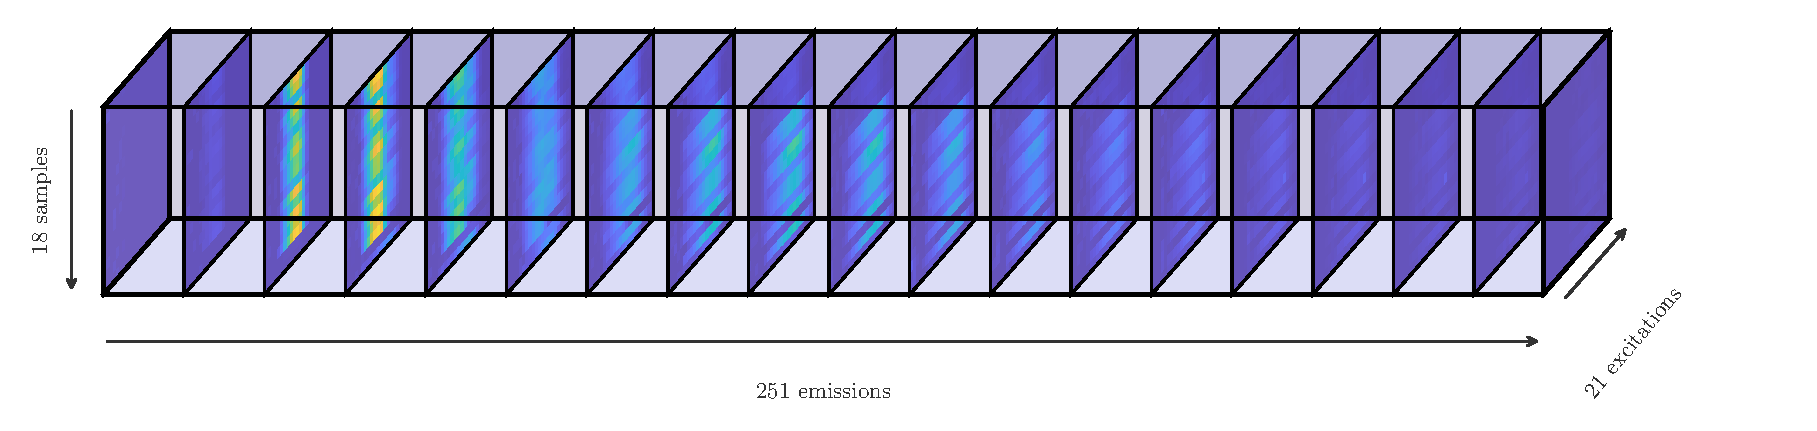
\includegraphics[width=0.85\textwidth]{Sources/Chapter4/figures/piled_tensor.pdf}
	\caption{Rappresentazione tridimensionale del tensore EEM di dimensioni $18 \times 251 \times 21$.}
	\label{fig:piled_tensor}
\end{figure}

\begin{figure}[htbp]
	\centering
	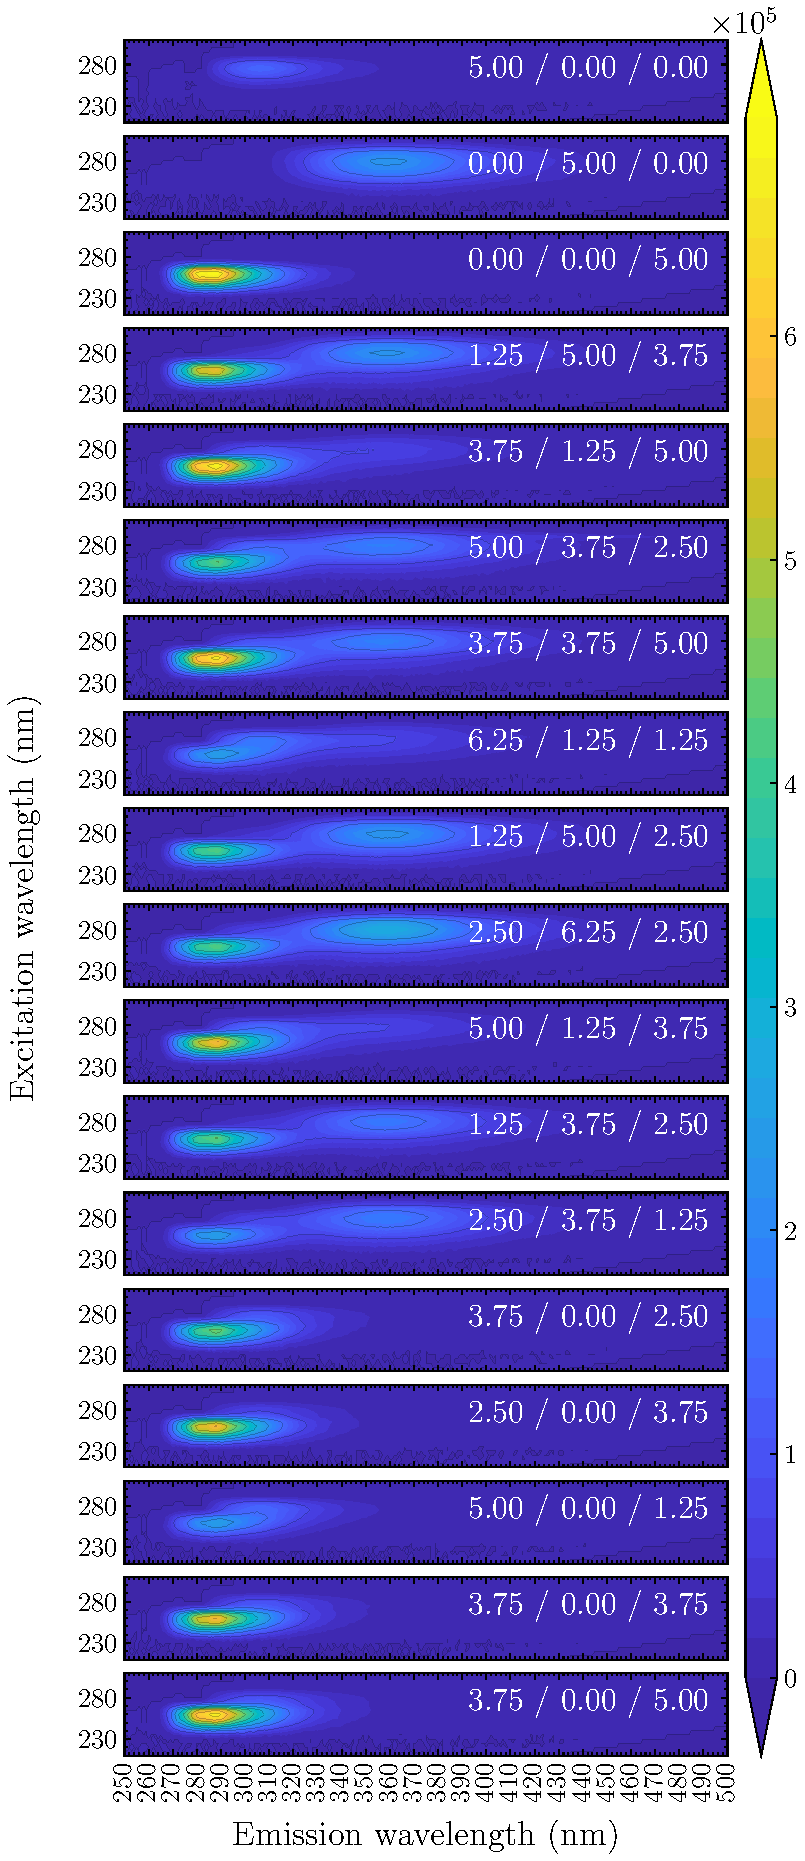
\includegraphics[width=0.60\textwidth]{Sources/Chapter4/figures/X-slices.pdf}
	\caption{Profili d'intensità di emissione-eccitazione del tensore EEM. I profili rappresentano le
		matrici EEM e corrispondono
		alle fette orizzontali del tensore, ordinate dall'alto ($ T_{1,:,:} $) al basso ($ T_{18,:,:}
		$).
		Ogni fetta è etichettata a destra con le concentrazioni dei tre composti chimici
		(Val-Tyr-Val/Trp-Gly/Phe), e copre $ 21 $ lunghezze d'onda d'eccitazione per $ 251 $ lunghezze
		d'onda di emissione.}
	\label{fig:x_slices}
\end{figure}


Cerchiamo una fattorizzazione approssimata di $ \hat{T} $ con le tecniche descritte nella \S~\ref{sec:computing_cp}. Fissata una
tolleranza $ \varepsilon $ piccola, applichiamo il procedimento
dell'Algoritmo~\ref{alg:tensor_approx}. La ricerca di $ \hat{T} $ viene ripetuta attraverso una
serie di restarts per evitare minimi locali, al termine dei quali viene restituito il tensore che
minimizza l'errore relativo $ \varepsilon_{\text{rel}} $. Nell'articolo originale~\cite{smilde2004multi} vengono anche esclusi i tensori che non sono
ragionevoli da un punto di vista fisico per rimuovere valori di $ r $ troppo piccoli. Per i nostri scopi ci limitiamo a imporre che le quantità fisiche coinvolte (concentrazioni, intensità di emissione ed eccitazione) siano non negative, per cui si scartano le decomposizioni che presentano fattori negativi.

\begin{algorithm}[htbp]
	\caption{Algoritmo di approssimazione del tensore originale.}
	\label{alg:tensor_approx}
	\begin{algorithmic}[1]
		\For{$i = 1 \dots r$}
		\Repeat
		\State $\hat{T} \gets \arg\min_{A, B, C} \nrm{T - \dsqr{A, B, C}}$ \Comment{CP ALS con restarts.}
		\Until{$\nrm{T - \hat{T}} < \varepsilon$}
		\EndFor
	\end{algorithmic}
\end{algorithm}

\begin{figure}[htbp]
	\centering
	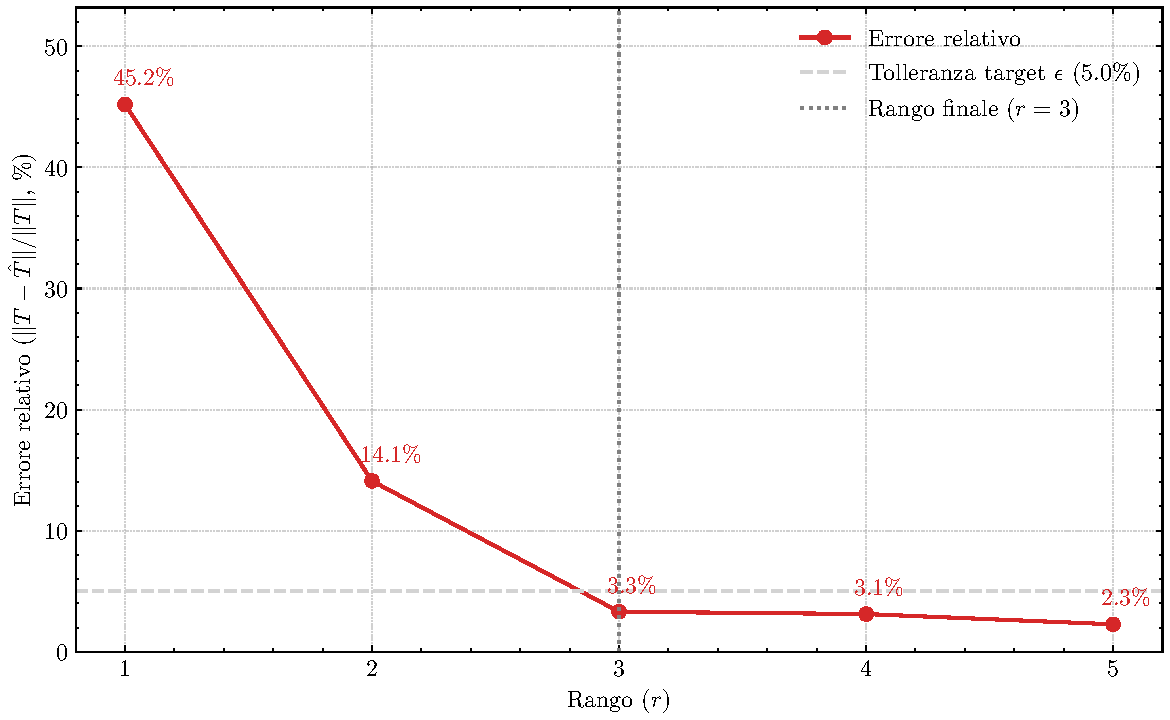
\includegraphics[width=0.7\textwidth]{Sources/Chapter4/figures/eem_cp_error_vs_rank.pdf}
	\caption{Errore relativo al variare del rango della decomposizione approssimante. Il rango
		ottimale selezionato è $r = 3$, corrispondente al superamento della tolleranza target
		$\varepsilon = 0.05$. Osserviamo che la precisione non varia di molto all'aumentare di $ r $.}
	\label{fig:eem_cp_error_vs_rank}
\end{figure}

Assumiamo ora che il rango ottimale $ r $ sia stato determinato attraverso l'euristica discussa in
\S~\ref{sec:computing_rank}. Siccome i valori di $ r $ sono relativamente piccoli,
a meno di piccole perturbazioni, l'espressione di $ \hat{T} $ come somma di elementi di rango uno
sarà unica grazie al Teorema di Kruskal~\ref{thm:kruskal3d}. Quindi, decomponendo $ \hat{T} $,
possiamo recuperare la concentrazione
di ognuna delle $ r $ sostanze in ogni soluzione, determinando i vettori $ a_{f} $ così come lo
spettro delle eccitazioni ed emissioni determinando i vettori $ b_{f} $.
La Figura~\ref{fig:eem_model} mostra i fattori calcolati e il confronto con le concentrazioni reali
delle tre sostanze, arrestando CP ALS quando la differenza dell'errore relativo tra due iterazioni
susseguenti è minore di $ 10^{-4} $. Nel grafico sono tracciati i fattori $ a_{f},b_{f},c_{f} $ della decomposizione
CP, dove ogni riga $ f  = 1,2,3 $ rappresenta una sostanza diversa (scritta in sottoimpressione). Ad
esempio, la componente $ a_1 $ sono le barre blu nella prima sottofigura in alto a sinistra, dove
notiamo che i primi due fattori di $ a_{1} $ sono nulli, che significa che la componente non è
presente nei primi due campioni. Nella colonna centrale in alto denotiamo le componenti individuali di $ b_1
$, che sono $ 256 $, con dei punti. Il terzo fattore $ c_1 $ è rappresentato nella figura in alto a
destra. Analogamente la seconda riga descrive i fattori $ a_2,b_2,c_2 $ e la terza $ a_3,b_3, c_3 $.
Nel calcolo della fattorizzazione abbiamo dovuto riscalare i fattori del tensore ottenuto da ALS per
mantenere i valori fedeli al tensore originale. Inoltre abbiamo permutato i fattori con un algoritmo
simile a quello che descriveremo nella \S~\ref{sec:num_experiment_omini}.\todo{Serve precisare
	meglio?}


\begin{figure}[htbp]
	\centering
	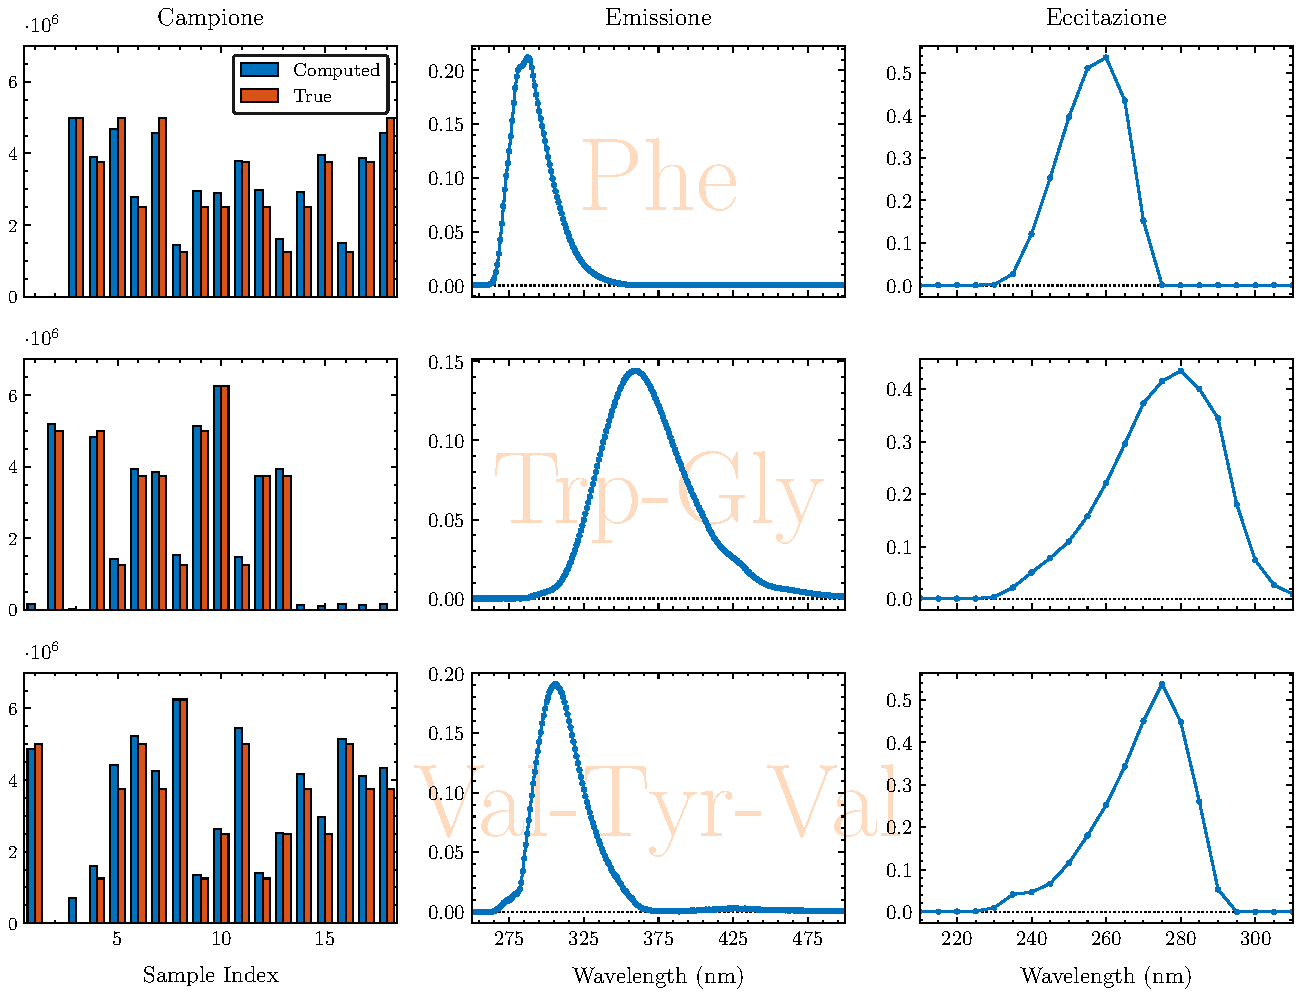
\includegraphics[width=1\textwidth]{Sources/Chapter4/figures/eem_model.pdf}
	\caption{Fattori della decomposizione CP non negativa a rango $r=3$ del tensore EEM. I diagrammi a barre a sinistra confrontano i profili di concentrazione calcolati con le concentrazioni effettive delle tre sostanze (Val-Tyr-Val, Trp-Gly, Phe).}
	\label{fig:eem_model}
\end{figure}

\pagebreak

\section{Blind source separation}

Immaginiamo una stanza affollata in cui diverse persone parlano contemporaneamente, mentre alcuni
microfoni sparsi per la sala che registrano le
conversazioni. Poiché i microfoni catturano solo la sovrapposizione delle singole voci, l'obiettivo
è elaborare le registrazioni per isolare la voce di ogni singola persona. Questo scenario è noto
nell'analisi di segnali come \emph{blind source separation}.

In questa sezione studieremo un problema simile utilizzando la decomposizione CP. In particolare, ci
concentreremo su un'applicazione nel campo delle telecomunicazioni wireless nota come \emph{blind
	deconvolution} nel modello \emph{direct-sequence code-division multiple
	access} (DS-CDMA)~\cite{sidiropoulos2000blind,de2008blind,landsberg2011tensors} che riadattiamo in
questa sezione.

Per semplicità supponiamo che $ R $ utenti mandino dei messaggi a $ I $ antenne. I messaggi arrivano
mischiati, e l'obiettivo è recuperare i segnali individuali e le posizioni degli utenti.


\begin{figure}[htbp]
	\centering
	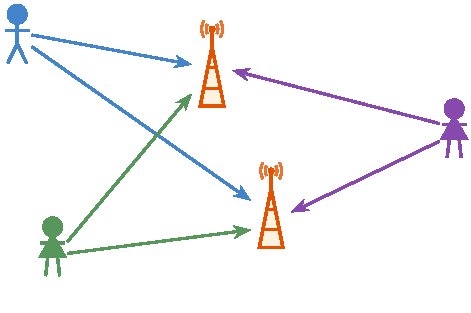
\includegraphics{Sources/Chapter4/figures/antennae.pdf}
	\caption{$R = 3$ sorgenti inviano segnali a $I = 2$ antenne.}
	\label{fig:antennae}
\end{figure}

L'utente $ r $-esimo trasmette il messaggio in un vettore di $ s_{r} = \left[ s_{1r}, \ldots, s_{Kr}
		\right]^{\top}  \in \R^{K}$, dove le entrate sono numeri reali random. Ci sono $ I $ antenne che ricevono i segnali.
Quando i segnali arrivano all'$ i $-esima antenna, il segnale ha subito distorsione
nella sua intensità e fase (anche detta \emph{fading/gain}), quindi ciò che viene ricevuto dall'antenna $
	i $-esima sono le $ IK $ quantità $ a_{ir}s_{kr} $, dove $ a_{ir} $ è il fading/gain tra l'utente $
	r $ e l'antenna $ i $.

In questo scenario si riceve un tensore (matrice) $ T \in \C^{I \times K} $ di rango $ R $ di entrate
\begin{equation*}
	T_{ik} = \sum_{r=1}^R a_{ir}s_{kr}.
\end{equation*}
L'obiettivo sarebbe recuperare i segnali $ s_{r} $, per $ 1\le r \le R $ da questa
matrice decomponendola come somma di matrici di rango uno. Sfortunatamente, questa decomposizione non è mai
unica quando $ R > 1 $. Per aggirare il problema, vengono introdotti dei ``codici'' per ``diffondere'' il segnale che
ogni utente invia per ottenere un tensore a tre indici che avrà generalmente una decomposizione
unica.\footnote{Tale spreading è comune nelle telecomunicazioni, e.g. della ridondanza è introdotta per
	compensare gli errori causati dalla corruzione dei segnali durante la trasmissione.}

Facciamo le seguenti ipotesi sulla trasmissione dei segnali: la trasmissione avviene in linea
d'aria, seguendo la strada più breve (secondo la distanza euclidea) senza incontrare ostacoli; i
simboli inviati arrivano in maniera ordinata senza sovrapposizione (esempio $ s_{k,r} $ allo stesso
tempo di $ s_{k+1,r} $). Questi comportamenti sono noti in letteratura come ICI (\emph{interchip
	interference}) e ISI (\emph{intersignal interference}).
Inoltre i segnali non subiscono rumore e non vengono memorizzati.

Per recuperare $ s_{r}
$ e $ a_{ir} $, l'$ r $-esimo utente
introduce una ridondanza in termini di codice chiamata \emph{spreading sequence} che è fissata per
ogni utente, diciamo $ c_{r} = \left[ c_{1r}, \ldots, c_{Jr} \right]^{\top} $. Vengono trasmesse simultaneamente $ J $ quantità
$ \left[ s_{kr}c_{1r}, \ldots, s_{kr}c_{Jr} \right] $, chiamate \emph{chips} al tempo $ k $, dove in
ogni entrata rappresenta la trasmissione del simbolo $ s_{kr} $ su una frequenza diversa. La
trasmissione totale sopra $ JK $ unità di tempo dell'utente $ r $-esimo sono le $ JK $ chips $
	c_{jr}s_{kr} $, $ 1 \le j \le J $, $ 1\le k \le K $ (qui $ J $ è anche detto \emph{spreading gain}).
L'antenna $ i $-esima riceve le $ JK $ quantità $ \sum_{r} a_{ir}c_{jr}s_{kr} $, per $ 1 \le j \le J
$, $ 1 \le k \le K $, dove, come sopra, $ a_{ir} $ sono i fading/gain tra l'utente $ r $ e l'antenna
$ i $. In totale, viene ricevuto un tensore $ T \in \C^{I \times J\times K} $ di rango $ R $
scrivibile in componenti come
\begin{equation}
	\label{eq:blindec_cp_components}
	T_{ijk} = \sum_{r=1}^R a_{ir}c_{jr}s_{kr},
\end{equation}
o in generale,
\begin{equation*}
	T = \sum_{r=1}^R a_{r} \otimes c_{r} \otimes s_{r}.
\end{equation*}
In altre parole, $ T = \dsqr{S,C,A} $. L'obiettivo è recuperare i segnali $ s_{r} $, per $ 1\le r\le
	R $ da questo tensore, cioè la matrice $ S $. Per farlo abbiamo bisogno che la scrittura sia
essenzialmente unica. Per il Teorema di Kruskal~\ref{thm:kruskal3d} questa decomposizione è unica se
\begin{equation*}
	\krk{A} + \krk{B} + \krk{C} \ge 2(R+1).
\end{equation*}
Per costruzione~\cite{de2008blind} le matrici $ A $ e $ C $ sono di $ k $-rango pieno con probabilità $ 1
$, mentre se i simboli trasmessi $ s_{Kr} $ appartengono ad un alfabeto finito, c'è possibilità che
$ S $ non sia di $ k $-rango pieno---c'è una possibilità che le sequenze di utenti diversi possano essere
uguali, ma questo è poco probabile per dataset più grandi. Quindi nella pratica assumiamo che $ S $
sia di $ k $-rango pieno. Questo significa che il numero di utenti che possono essere processati
simultaneamente si può considerare limitato come
\begin{equation}
	\label{eq:krk_eq_full_rank}
	\min \{I,R\} + \min \{J,R\} + \min \{K,R\} \ge 2(R+1).
\end{equation}

Il calcolo di $ T $ avviene con l'Algoritmo ALS~\ref{alg:ALS}.

\begin{remark}
	Una limitazione di questo modello è che in ambito industriale spesso ci sono poche antenne e meno
	utenti, quindi si perde l'unicità.
\end{remark}

\subsection*{Esperimento numerico}
\label{sec:num_experiment_omini}

Consideriamo lo scenario dove $ R = 4 $ utenti vogliono inviare messaggi di $ K = 100 $ simboli a $
	I = 5 $ antenne, con un fattore di spreading $ J = 16 $.
Generiamo dei tensori
\begin{equation*}
	T_{\sigma} = T_{\text{clean}} + W_{\sigma} \in \R^{I\times J\times K}
\end{equation*}
dove $ W_{\sigma} $ è un tensore di rumore gaussiano con entrate in $ \mathcal{N}(0, \sigma) $ e $
	T_{\text{clean}} $ è un tensore generato in formato denso a partire dalla decomposizione $
	T_{\text{clean}} = \dsqr{A,C,S}$. L'esperimento consiste in recuperare la posizione degli $ R $
utenti conoscendo la posizione delle antenne (la matrice $ A $). Per farlo dobbiamo calcolare le
matrici $ S $ e $ C $, sfruttando la decomposizione CP al variare del rumore $ \sigma $ nella
Tabella~\ref{tab:dscdma_noise_scale}.

\begin{table}[htbp]
	\centering
	\caption{Livelli di rumore gaussiano applicati al tensore $T_{\sigma} = T_{\text{clean}} + W_{\sigma}$, con relativo rapporto segnale-rumore (SNR) e corrispondente scenario fisico di trasmissione.}
	\label{tab:dscdma_noise_scale}
	\begin{tabular}{c c c c l}
		\toprule
		Rumore     & $\sigma$   & $\text{SNR}_{\text{dB}}$ & Scenario fisico       \\
		\midrule
		$\sigma_0$ & $0{,}0000$ & $\infty\text{ dB}$       & Assenza di rumore     \\
		$\sigma_1$ & $0{,}0173$ & $16{,}5\text{ dB}$       & Segnale ottimo        \\
		$\sigma_2$ & $0{,}0403$ & $9{,}1\text{ dB}$        & Segnale buono         \\
		$\sigma_3$ & $0{,}0691$ & $4{,}4\text{ dB}$        & Segnale debole        \\
		$\sigma_4$ & $0{,}1037$ & $0{,}9\text{ dB}$        & Segnale quasi assente \\
		$\sigma_5$ & $0{,}1382$ & $-1{,}6\text{ dB}$       & Fortissime
		interferenze                                                               \\
		\bottomrule
	\end{tabular}
\end{table}


\begin{itemize}
	\item Matrice delle antenne $ A \in \R^{I \times R}$: generiamo le posizioni delle antenne $ p_{i}
	      $ e degli utenti $ u_{r} $ nel quadrato $ [0,L]^2 $, dove $ L $ è un generico intero
	      positivo, per $ i = 1, \ldots, I $ e $ r = 1, \ldots, R $. Le entrate di $ A $ sono $ a_{ir}
		      \defeq \frac{1}{\| p_{i} - u_{r} \|_{2}}$, dove assumiamo che $ \| p_{i} - u_{r} \|_{2} >
		      0$ (gli utenti non si trovano sulle antenne).
	\item Matrice dei simboli $ S \in \R^{K \times R} $ con entrate $ s_{kr} $ secondo la
	      distribuzione gaussiana standard
	      $ \mathcal{N}(0,1) $.
	\item Matrice delle sequenze di spreading $ C \in \{-1,1\}^{J \times R}  $: contiene i codici
	      casuali assegnati a ciascuna delle $ R $ sorgenti, dove $ c_{jr} = -1 $ o $ c_{jr} = 1 $ con
	      uguale probabilità.
\end{itemize}
L'Algoritmo ALS~\ref{alg:ALS} produce un tensore approssimante $ \hat{T} = \dsqr{\hat{A}, \hat{C},
		\hat{S}} $ unico a meno di permutazione e riscalamento dei fattori: per i valori scelti, l'Equazione~\ref{eq:krk_eq_full_rank} è
verificata in senso stretto. In questa applicazione è importante recuperare l'ordine dei
fattori---altrimenti un utente finirebbe per trovarsi sulla posizione di un altro utente.
Descriviamo ad alto livello il procedimento per recuperare la permutazione originale. Indichiamo con $ (a_{r},c_{r},s_{r}) $ i fattori di $ T $ e
con $ (\hat{a}_{r}, \hat{c}_{r}, \hat{s}_{r}) $ i fattori di $ \hat{T} $.
\begin{enumerate}
	\item Calcoliamo correlazione tra ogni colonna $ \hat{a}_{k} $ e $ a_{r} $ tramite $ \rho_{kr}
		      \defeq \frac{\hat{a}^{\top}_{k}a_{r}}{\|\hat{a}_{k}\|_{2} \cdot \|a_{r} \|_{2}}$.
	\item Costruiamo la matrice dei costi $ M \in \R^{R\times R} $ di entrate $ M_{kr} = 1 -
		      \abs{\rho_{kr}} $.
	\item Troviamo una permutazione ottima $ \pi^* \in \mathfrak{S}_{R} $ che realizza
	      \begin{equation*}
		      \min_{\pi \in \mathfrak{S}_{R}} \sum_{r=1}^R M_{\pi(r),r}.
	      \end{equation*}
	\item Calcoliamo il cambio di segno tramite $ \xi_{r} \defeq
		      \mathop{sign}(\hat{a}^{\top}_{\pi^*(r)}a_{r}) \in \{-1,1\} $.
	\item Permutiamo e riscaliamo $ \hat{A} $ e $\hat{S} $ applicando $ \xi_{r}\hat{A}_{:, \pi^*(r)} $ e
	      $ \xi_{r}\hat{S}_{:, \pi^*(r)} $, rispettivamente.
\end{enumerate}

\subsection*{Risultati}

Nel contesto definito sopra, denotiamo gli utenti reali $ r \in \{1, \ldots, R\}  $ con dei quadrati
e gli utenti recuperati con degli omini dello stesso colore. Inizialmente verifichiamo che in
assenza di rumore l'utente recuperato combaci con l'utente reale, come illustrato in
Figura~\ref{fig:antenna_localization_plot}. Inoltre verifichiamo che ciò funzioni per diverse
disposizioni degli utenti e delle antenne in Figura~\ref{fig:dscdma_6_experiments}. Di seguito,
generiamo più tensori $ T_{\sigma} $ al variare di $ \sigma $ nella
Tabella~\ref{tab:dscdma_noise_scale} e osserviamo quanto gli utenti recuperati si discostano
dall'utente originale. In Figura~\ref{fig:dscdma_noise_experiment} osserviamo i comportamenti tipici
di deriva al crescere del rumore. Infine, la Figura~\ref{fig:dscdma_noise_experiment_multi} mostra
ulteriori esecuzioni dell'algoritmo su sei configurazioni spaziali differenti.

\begin{figure}[htbp]
	\centering
	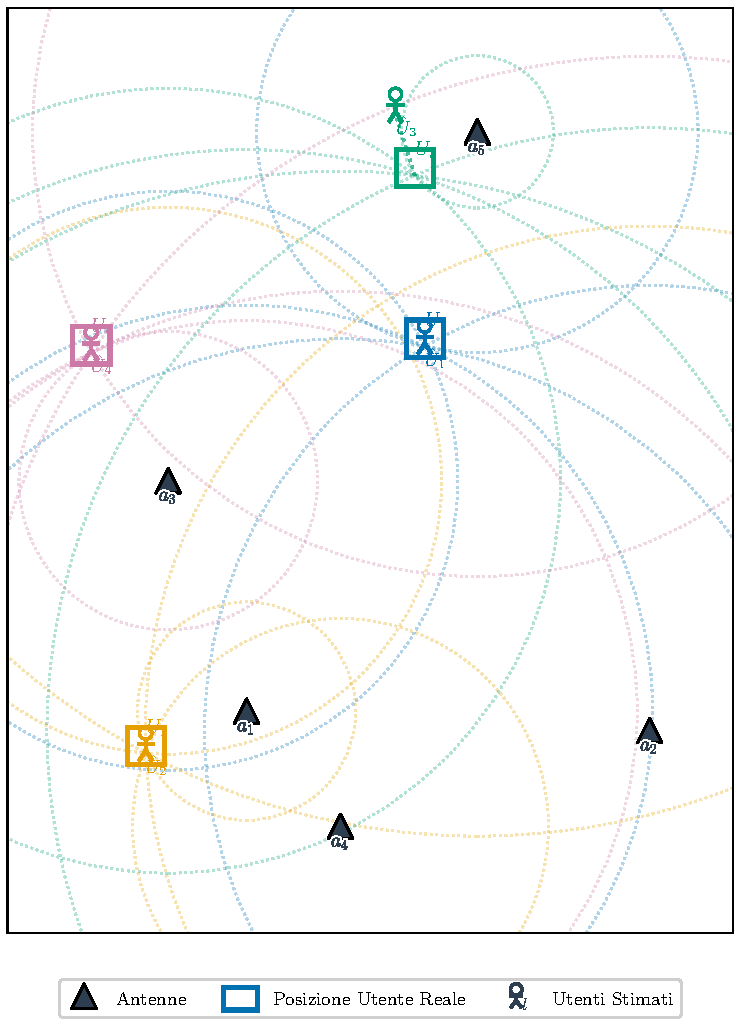
\includegraphics[width=1\textwidth]{Sources/Chapter4/figures/antenna_localization_plot.pdf}
	\caption{Stima della posizione degli utenti e delle antenne in assenza di rumore. I quadrati trasparenti indicano le posizioni reali degli utenti $U_r$, gli omini indicano le posizioni stimate $\hat{U}_r$, i triangoli scuri indicano le antenne $a_i$, e le circonferenze tratteggiate indicano le distanze stimate dalle antenne.}
	\label{fig:antenna_localization_plot}
\end{figure}

\begin{figure}[htbp]
	\centering
	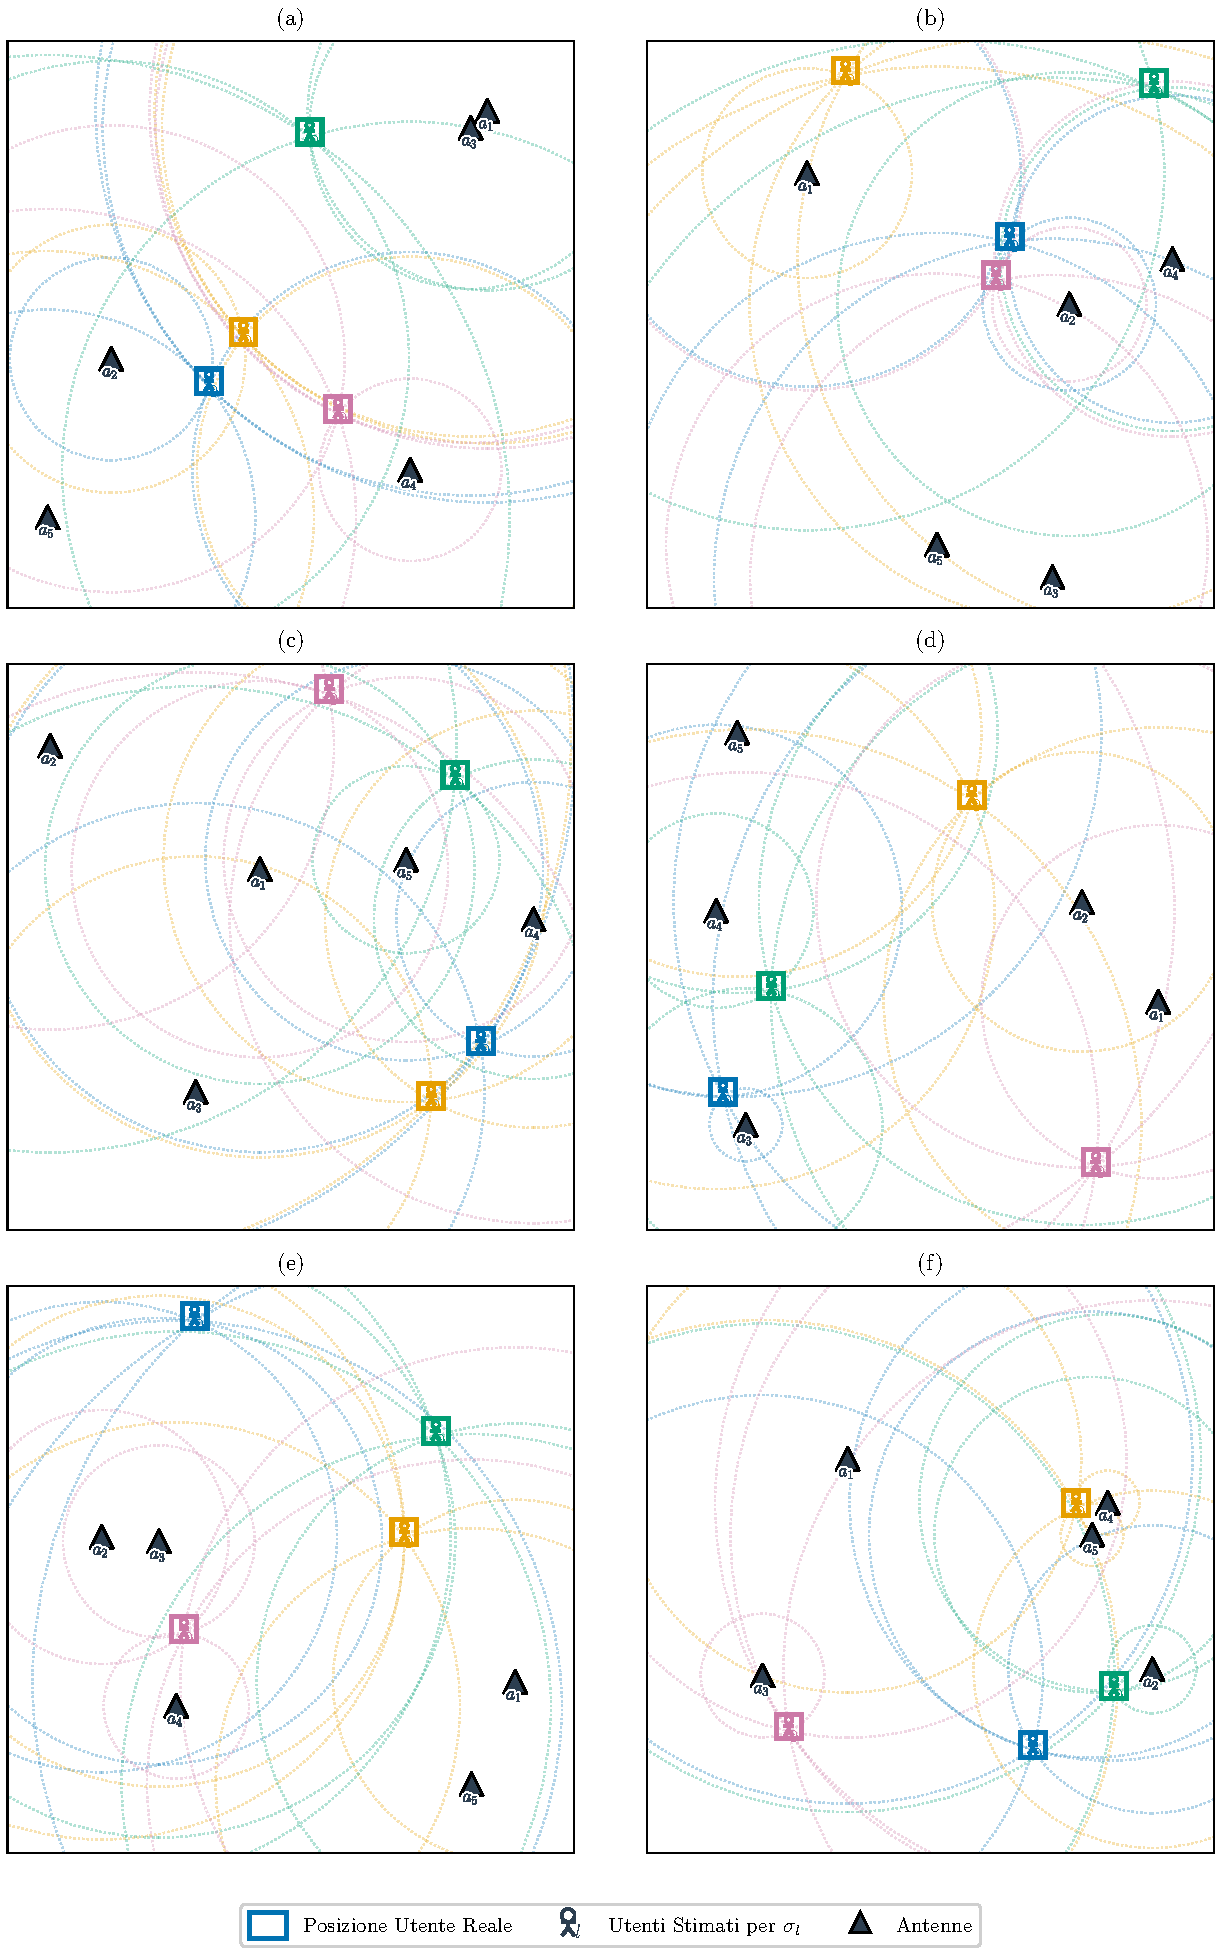
\includegraphics[width=\textwidth]{Sources/Chapter4/figures/dscdma_6_experiments.pdf}
	\caption{Stima della posizione degli utenti e delle antenne in sei esperimenti indipendenti con diverse disposizioni spaziali di antenne e sorgenti in assenza di rumore.}
	\label{fig:dscdma_6_experiments}
\end{figure}

\begin{figure}[htbp]
	\centering
	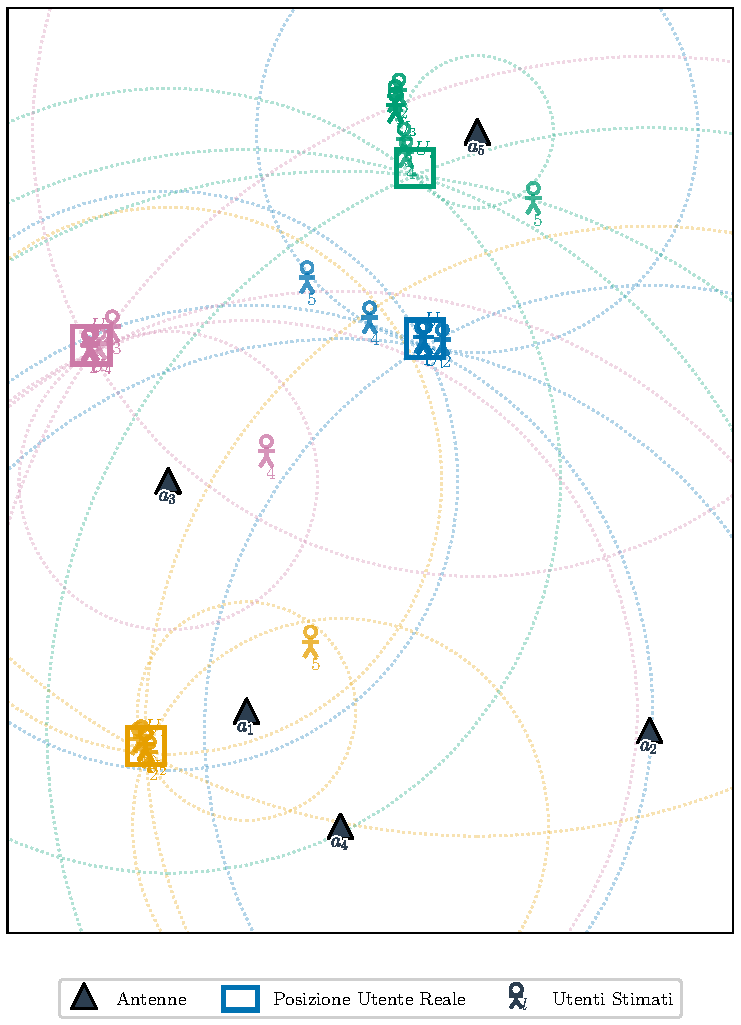
\includegraphics[width=\textwidth]{Sources/Chapter4/figures/dscdma_noise_experiment.pdf}
	\caption{Deriva della localizzazione degli utenti sotto sei livelli crescenti di rumore gaussiano ($\sigma_0, \ldots, \sigma_5$) per un singolo esperimento. Gli omini numerati da $1$ a $5$ indicano le posizioni stimate al crescere del livello di rumore.}
	\label{fig:dscdma_noise_experiment}
\end{figure}

\begin{figure}[htbp]
	\centering
	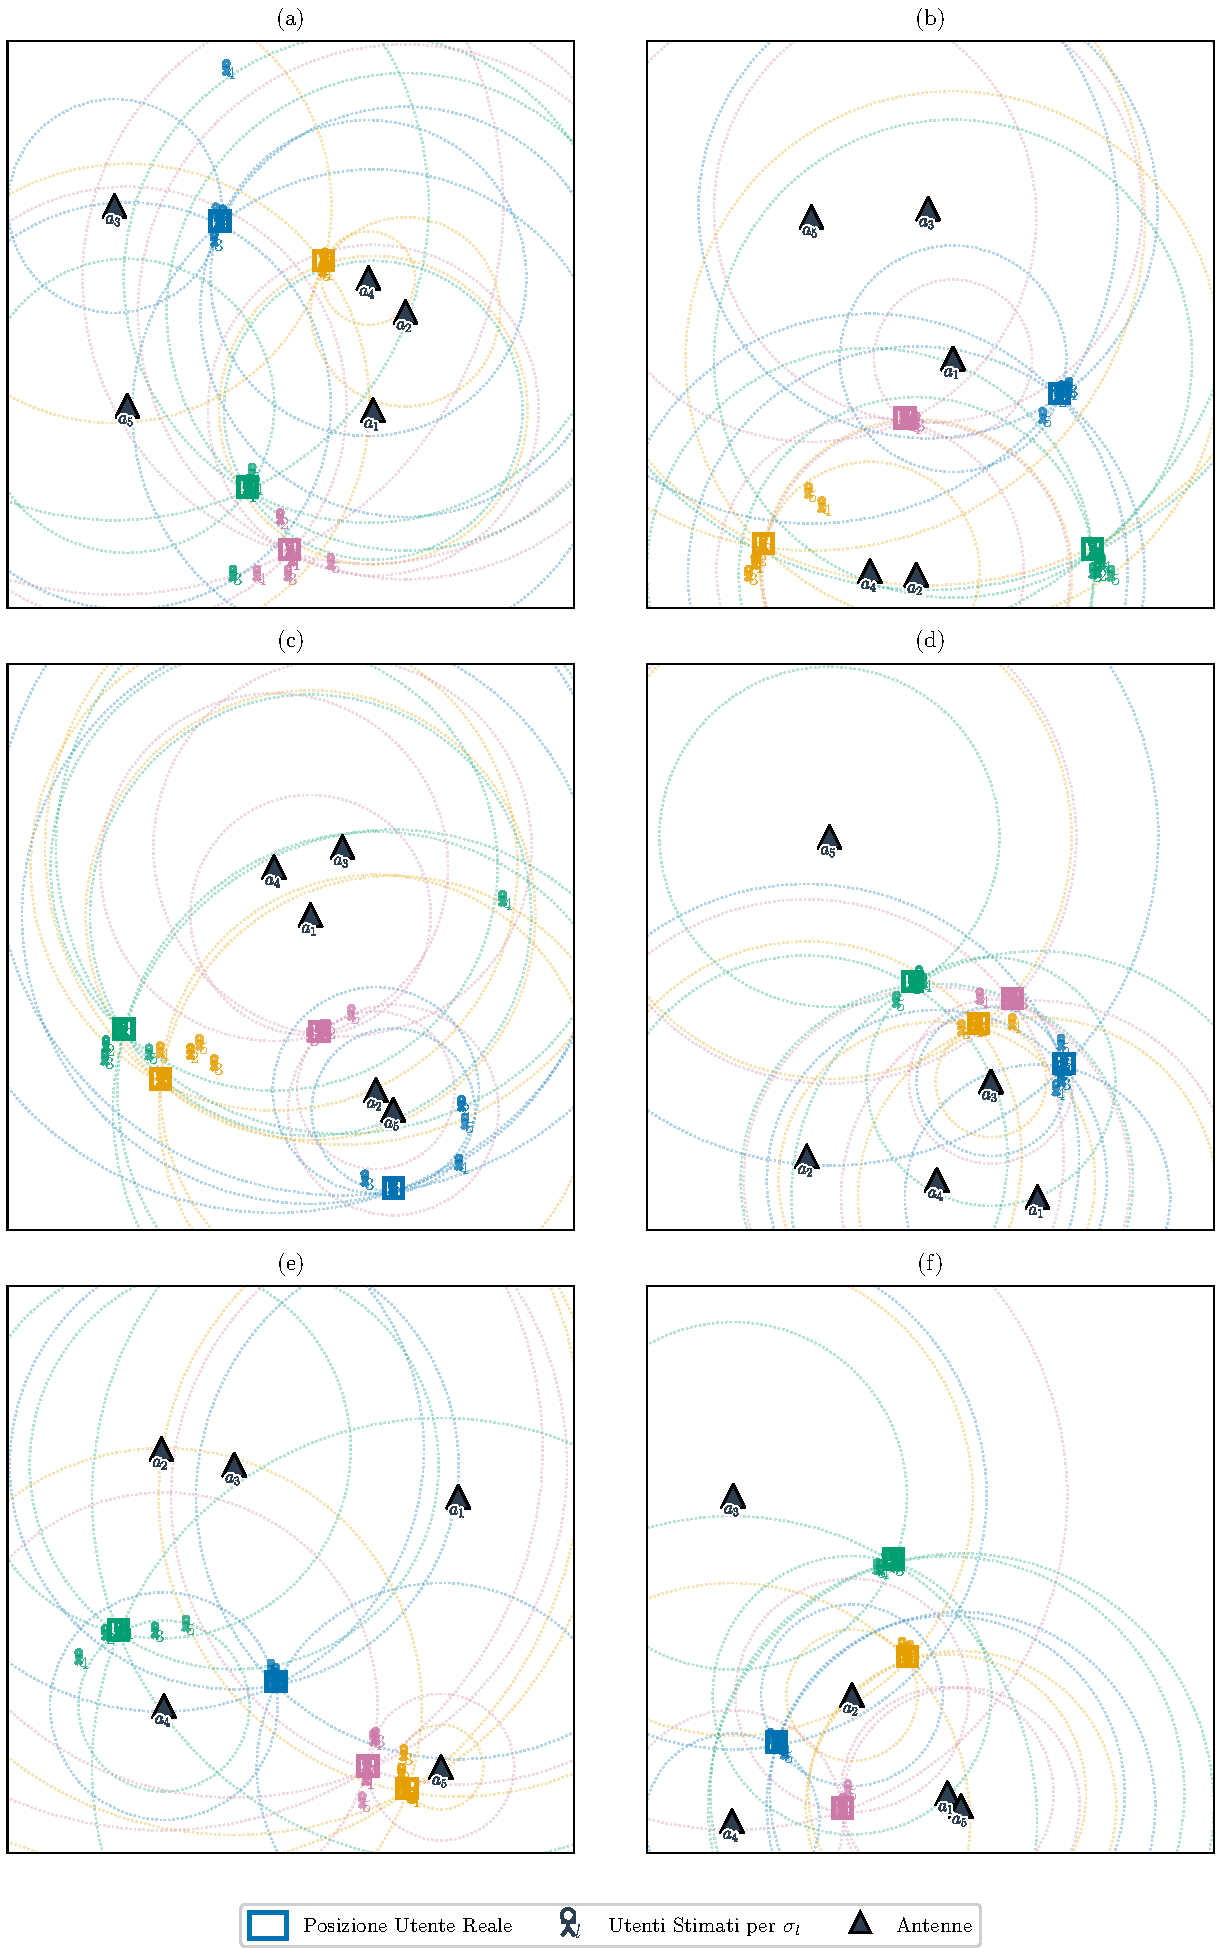
\includegraphics[width=\textwidth]{Sources/Chapter4/figures/dscdma_noise_experiment_multi.pdf}
	\caption{Deriva della localizzazione degli utenti sotto rumore gaussiano per sei esperimenti indipendenti (disposizioni spaziali differenti), mostrando i comportamenti tipici di deriva al crescere del livello di rumore $\sigma_l$.}
	\label{fig:dscdma_noise_experiment_multi}
\end{figure}

% %%%%%%%%%%%%%%%%%%%%%%%%%%%%%%%%%%%%%%%%%%%%%%%%%%%%%%%%%%%%%%%%%%%%%%%%
\chapter{Appendice}
%%%%%%%%%%%%%%%%%%%%%%%%%%%%%%%%%%%%%%%%%%%%%%%%%%%%%%%%%%%%%%%%%%%%%%%%

\section{Il master method}

Introduciamo brevemente un metodo per risolvere relazioni ricorsive definite per ricorrenza, detto
\emph{master method}. I lettori più interessati possono trovare una trattazione più dettagliata sul
libro~\cite{cormen2022introduction}. Il master method si usa per risolvere ricorrenze della forma
\begin{equation}
  \label{eq:master_rec}
  T(n) = aT(\frac{n}{b}) + f(n),
\end{equation}
dove $ a \ge 1 $ e $ b>1 $ sono costanti e $ f(n) $ è una funzione asintoticamente positiva. La
ricorrenza \ref{eq:master_rec} descrive il tempo di esecuzione di un algoritmo che divide un
problema di dimensione $ n $ in $ a $ sottoproblemi, ognuno di dimensione $ \frac{n}{b} $. Gli $ a $
sottoproblemi vengono risolti ricorsivamente in tempo $ T(\frac{n}{b}) $, e la funzione $ f(n) $
rappresenta il costo di dividere il problema e ricombinare la ricorsione di ogni sottoproblema.

\begin{definition}[Notazione $ O-$grande/piccolo]
  Per delle funzioni $ f,g $ a variabile reale (o intera) nella variabile $ x $ diciamo che:
  \begin{itemize}
    \item $ f(x) = O(g(x)) $ se esiste una costante $ C > 0 $ e un valore $ x_0 $ tale che $ |f(x)|
    \le C|g(x)| $ per ogni $ x\ge x_0 $.
  \item $ f(x) = o(g(x)) $ se $ \lim_{x \to \infty } \frac{|f(x)|}{|g(x)|} = 0 $.
  \item $ f(x) = \Omega(g(x))$ se esiste una costante $ C>0 $ e un valore $ x_0  $ tale che $
    C|f(x)| \ge |g(x)| $ per ogni $ x\ge x_0 $.
  \item $ f(x) = \omega(g(x)) $ se $ \lim_{x \to \infty } \frac{|g(x)|}{|f(x)|} = 0 $.
  \item $ f(x) = \Theta(g(x)) $ se $ f(x) = O(g(x)) $ e $ f(x) = \Omega(g(x)) $.
  \end{itemize}
  
\end{definition}

\begin{theorem}[Master theorem]
  \label{th:master}
  Siano $ a\ge 1 $ e $ b>1 $ delle costanti, sia $ f(n) $ una funzione e definiamo la legge
  ricorsiva $ T : \N \to \R $ con la ricorrenza
  \begin{equation*}
    T(n) = aT(\frac{n}{b}) + f(n),
  \end{equation*}
\end{theorem}
dove con $ \frac{n}{b} $ indichiamo sia $ \left\lfloor \frac{n}{b} \right\rfloor $ o $ \left\lceil
\frac{n}{b} \right\rceil  $. Allora $ T(n) $ assume i seguenti comportamenti asintotici: 
\begin{enumerate}
  \item Se $ f(n) = O(n^{\log_b a-\varepsilon}) $ per qualche $ \varepsilon >0 $, allora $ T(n) =
    \Theta(n^{\log_b a}) $.
  \item Se $ f(n) = \Theta(n^{\log_b a}) $ allora $ T(n) = \Theta(n^{\log_b a \log n}) $.
  \item If $ f(n) = \Omega(n^{\log_b a + \varepsilon}) $ per qualche costante $ \varepsilon >0 $, e
    se $ af(\frac{n}{b}) < cf(n) $ per qualche costante $ c<1$ e ogni $ n $ sufficientemente grande,
    allora $ T(n) = \Theta(f(n)) $.
\end{enumerate}

\begin{example}
  Nel caso dell'algoritmo naive la ricorrenza ha la forma $ a = 8 $, $ b = 2 $ e $ f(n) =
  \Theta(n^2) $, ovvero
  \begin{equation*}
    T(n) = 8T(\frac{n}{2}) + \Theta(n^2).
  \end{equation*}
  Siccome $ n^{\log_b a} = n^{\log_2 8} = n^3 $, che è polinomialmente più grande di $ f(n) $, ovvero $
  f(n) = O(n^{3-\varepsilon}) $ per $ \varepsilon = 1 $, dal caso 1 di \ref{th:master} segue che $
  T(n) = \Theta(n^3) $.
  Nel caso di Strassen, si ripetono i calcoli con $ a = 7 $, $ b=2 $ e $ f(n) = \Theta(n^2) $ e si
  ottiene la relazione $ T(n) = 7T(\frac{n}{2}) + \Theta(n^2)$ e analogamente $ T(n) =
  \Theta(n^{\log_2 7}) $.
\end{example}




% This ensures that the subsequent sections are being included as root
% items in the bookmark structure of your PDF reader.
\bookmarksetup{startatroot}
\backmatter

\begingroup
\let\clearpage\relax
\renewcommand{\glsgroupskip}{}
\glsaddall
\printglossary[type=\acronymtype]
\newpage
\printglossary
\endgroup

\printindex
\printbibliography

\end{document}
